%%%%%%%%%%%%%%%%%%%%%%%%%%%%%%%%%%%%%%%%%%%%%%%%%%%%%%%%%%%%%%%%%%%%%%%%%%%%%%%%
% University of Western Ontario Thesis Template
% By: Justin Quinn Veenstra, 2010
% With thanks to Mr. (soon to be Dr.) Will Robertson.


\documentclass[12pt,twoside]{report}
%% Decomment next line to use PostScript fonts
%%\UsePackage{times}
%%%%%%%%%%%%%%%%%%%%%%%%%%%%%%%%%%%%%%%%%%%%%%%%%%%%%%%%%%%%%%%%%%%%%%%%
%%                                                                    %%
%%                    ***   I M P O R T A N T   ***                   %%
%%                                                                    %%
%% Fill in the following fields with the required information:        %%
%%  - \department{...}  name of the graduate department               %%
%%  - \degree{...}      name of the degree obtained                   %%
%%  - \author{...}      name of the author                            %%
%%  - \title{...}       title of the thesis                           %%
%%  - \gyear{...}       year of graduation                            %%
%%  - \super{...}    supervisor
%%  - \firstname, \middlename, \lastname... there is additional documentation by the actual fields, so I'll leave it at that
%%%%%%%%%%%%%%%%%%%%%%%%%%%%%%%%%%%%%%%%%%%%%%%%%%%%%%%%%%%%%%%%%%%%%%%%
\usepackage{appendix}
\usepackage{graphicx}
\usepackage{amsmath}
\usepackage[byname]{smartref}
%\usepackage{hyperref} %comment out for hardcopy
\usepackage{txfonts}
\usepackage{tocloft}


%My packages:
\usepackage{afterpage}
\usepackage{amssymb}
\usepackage{stmaryrd}
\usepackage{setspace}
\usepackage{attrib}
\usepackage{todonotes}
\usepackage{pgfplots}
\usepackage{subcaption}
%\usepackage{amsthm}
\usepackage{mdwlist}
\usepackage{listings}


\newtheorem{thm}{Theorem}[section]


%\newcommand{\fjoin}{\,\bar{\varobar}\,}
\newcommand{\fjoin}{\varobar}

\newcommand{\hset}[1]{ \left\{ \! \left| \; #1 \; \right| \! \right\} }

\newcommand{\hjoin}[1][]{\varobar^{#1}}

\newcommand{\restrict}[2]{\left.#1\right|_{#2}}

\newcommand{\outerproduct}{\boxtimes}

\newcommand{\oiClCl}[1]{{ 	[\![ #1 ]\!] }}
\newcommand{\oiClOp}[1]{{ 	[\![ #1 )\!) }}
\newcommand{\oiOpCl}[1]{{ 	(\!( #1 ]\!] }}
\newcommand{\oiOpOp}[1]{{	(\!( #1 )\!) }}

\newcommand{\op}{\star}

\newcommand{\supp}{\text{supp}}

\newcommand{\R}[1][]{\mathcal{R}_{#1}}
\newcommand{\C}[1][]{\mathcal{C}_{#1}}

\newcommand*\diff{\mathop{}\!\mathrm{d}}

\lstset{language=Pascal}
\lstset{morekeywords={try, catch, finally, fi, proc, local}}

\def\ind[#1]{1_{#1}}
\def\extendedreal{\bar{\mathbb{R}}}
\def\hsetover[#1]{\mathbb{Z}^{#1}}

\makeatletter
\numberwithin{figure}{chapter}
\newenvironment{acknowledgements}%
{\clearemptydoublepage
 \begin{center}
  \section*{Acknowledgements}
 \end{center}
 \begingroup
}{\newpage\endgroup}

\newenvironment{dedication}%
{\clearemptydoublepage 
 \begin{center}
  \section*{Dedication}
 \end{center}
 \begingroup
}{\newpage\endgroup}

\newenvironment{preliminary}%
{\pagestyle{plain}\pagenumbering{roman}}%
{\pagenumbering{arabic}}

\addtoreflist{chapter}
\newtheorem{theorem}{Theorem}[section]
\newtheorem{lemma}[theorem]{Lemma}
\newtheorem{proposition}[theorem]{Proposition}
\newtheorem{corollary}[theorem]{Corollary}

\newenvironment{proof}[1][Proof]{\begin{trivlist}
\item[\hskip \labelsep {\bfseries #1}]}{\end{trivlist}}
\newenvironment{definition}[1][Definition]{\begin{trivlist}
\item[\hskip \labelsep {\bfseries #1}]}{\end{trivlist}}
\newenvironment{example}[1][Example]{\begin{trivlist}
\item[\hskip \labelsep {\bfseries #1}]}{\end{trivlist}}
\newenvironment{remark}[1][Remark]{\begin{trivlist}
\item[\hskip \labelsep {\bfseries #1}]}{\end{trivlist}}

\newcommand{\qed}{\nobreak \ifvmode \relax \else
      \ifdim\lastskip<1.5em \hskip-\lastskip
      \hskip1.5em plus0em minus0.5em \fi \nobreak
      \vrule height0.75em width0.5em depth0.25em\fi}

% Default values for title page.

%% To produce output with the desired line spacing, the argument of
%% \spacing should be multiplied by 5/6 = 0.8333, so that 1 1/2 spaced
%% corresponds to \spacing{1.5} and double spaced is \spacing{1.66}.
\def\normalspacing{1.25} % default line spacing


%% Define the "thesis" page style.
\if@twoside % If two-sided printing.
\def\ps@thesis{\let\@mkboth\markboth
   \def\@oddfoot{}
   \let\@evenfoot\@oddfoot
   \def\@oddhead{
      {\sc\rightmark} \hfil \rm\thepage
      }
   \def\@evenhead{
      \rm\thepage \hfil {\sc\leftmark}
      }
   \def\chaptermark##1{\markboth{\ifnum \c@secnumdepth >\m@ne
      Chapter\ \thechapter. \ \fi ##1}{}}
   \def\sectionmark##1{\markright{\ifnum \c@secnumdepth >\z@
      \thesection. \ \fi ##1}}}
\else % If one-sided printing.
\def\ps@thesis{\let\@mkboth\markboth
   \def\@oddfoot{}
   \def\@oddhead{
      {\sc\rightmark} \hfil \rm\thepage
      }
   \def\chaptermark##1{\markright{\ifnum \c@secnumdepth >\m@ne
      Chapter\ \thechapter. \ \fi ##1}}}
\fi

\pagestyle{thesis}
% Set up page layout.
\setlength{\textheight}{9in} % Height of the main body of the text
\setlength{\topmargin}{-.5in} % .5" margin on top of page
\setlength{\headsep}{.5in}  % space between header and top of body
\addtolength{\headsep}{-\headheight} % See The LaTeX Companion, p 85
\setlength{\footskip}{.5in}  % space between footer and bottom of body
\setlength{\textwidth}{6.25in} % width of the body of the text
\setlength{\oddsidemargin}{.25in} % 1.25" margin on the left for odd pages
\setlength{\evensidemargin}{0in} % 1.25"  margin on the right for even pages

% Marginal notes
\setlength{\marginparwidth}{.75in} % width of marginal notes
\setlength{\marginparsep}{.125in} % space between marginal notes and text

% Make each page fill up the entire page. comment this out if you
% prefer. 
\flushbottom

\setcounter{tocdepth}{3} % Number the subsubsections 
\def\normalspacing{1.25} % default line spacing

\newcommand\isco[1]{%
  \edef\@tempa{#1}%
  \def\@tempb{}%
  \ifx\@tempa\@tempb
	\else \\\underline{Co-Supervisor:}\vspace{0.35in}\\\dots\dots\dots\dots\dots\dots\dots\\{#1}\\
  \fi
}

\newcommand\isjoint[1]{%
  \edef\@tempa{#1}%
  \def\@tempb{}%
  \ifx\@tempa\@tempb
	\else \\\underline{Joint Supervisor:}\vspace{0.35in}\\\dots\dots\dots\dots\dots\dots\dots\\{#1}\\
  \fi
}

\newcommand\isalt[1]{%
  \edef\@tempa{#1}%
  \def\@tempb{}%
  \ifx\@tempa\@tempb
	\else \\\underline{Alternate Supervisor:}\vspace{0.35in}\\\dots\dots\dots\dots\dots\dots\dots\\{#1}\\
  \fi
}

\newcommand\isdefinedsig[1]{%
  \edef\@tempa{#1}%
  \def\@tempb{}%
  \ifx\@tempa\@tempb
	\else \\ \dots\dots\dots\dots\dots\dots\dots\\{#1}\\
  \fi
}
\newcommand\isdefinedspinetitle[1]{%
  \edef\@tempa{#1}%
  \def\@tempb{}%
  \ifx\@tempa\@tempb
	\else (Spine title: #1)\\
  \fi
}
\newcommand\coauthor[1]{%
  \edef\@tempa{#1}%
  \def\@tempb{}%
  \ifx\@tempa\@tempb
	\else \newpage \Large Co-Authorship Statement\normalsize\\\indent\\#1\\
  \fi
}

\newcommand\acknowlege[1]{%
  \edef\@tempa{#1}%
  \def\@tempb{}%
  \ifx\@tempa\@tempb
	\else \newpage \Large Acknowlegements\normalsize\\\indent\\#1\newpage
  \fi
}

%\renewcommand{\appendixtocname}{\Huge \textbf{List of Appendices} \normalsize}
\newcommand{\blank}{\hspace{-2mm}}
\newcommand{\super}{Dr. S. M. Watt} %supervisor
\newcommand{\superj}{} %joint supervisor, if there is one, leave blank if not (lbin)... only one of the three.
\newcommand{\superc}{} %co-supervisor, if there is one, leave blank if not (lbin)
\newcommand{\supera}{} %alternate supervisor, if there is one, leave blank if not (lbin)
\newcommand{\sco}{}  %member of supervisory committee
\newcommand{\sct}{}  %other member of supervisory committee (lbin)
\newcommand{\examo}{}  %examining committee (up to four, if less leave blank)
\newcommand{\examt}{}
\newcommand{\examth}{}
\newcommand{\examf}{}
\newcommand{\department}{Computer Science}
\newcommand{\degree}{Masters of Science}
\newcommand{\firstname}{Mike}
\newcommand{\middlename}{}
\newcommand{\lastname}{Ghesquiere}
%\renewcommand{\author}[1]{\ifx\empty#1\else\gdef\@author{#1}\fi} 
\newcommand{\authorname}{{\firstname} {\middlename} {\lastname}}
\newcommand{\titl}{Domain Decomposition, Integration, and Inclusion-Exclusion}
\newcommand{\spinetitle}{}%only if the above is more than 60 characters
\newcommand{\thesisformat}{Monograph} %or Integrated Article
\newcommand{\gyear}{\number\year}
\newcommand{\makecoauthor}{
%Type information about coauthorship here/
}
\newcommand{\makeacknowlege} {
%Type in acknowlegements here
}
\newcommand{\listappendixname}{List of Appendices}
\newlistof{myappendices}{app}{\listappendixname}
\newcommand{\myappendices}[1]{%
\addcontentsline{app}{myappendices}{#1}\par}

\renewcommand{\maketitle}
{\begin{titlepage}
   \setcounter{page}{1}
   %% Set the line spacing to 1 for the title page.
   %\begin{spacing}{1} 
   \begin{large}
   \begin{center}
      \mbox{}
      \vfill
      {\MakeUppercase{\titl}}\\
      \isdefinedspinetitle{\spinetitle}
      (Thesis format: \thesisformat)\\
      \vfill
      by \\
      \vfill
      {\firstname} \underline{\lastname}\\
      \vfill
      Graduate Program in {\department}\\
      \vfill
		A thesis submitted in partial fulfillment\\
		of the requirements for the degree of\\
		\degree\\
		\vfill
		The School of Graduate and Postdoctoral Studies\\
		The University of Western Ontario\\
		London, Ontario, Canada\\
		\vfill
      {\copyright} {\authorname} {\gyear}  \\
      \vspace*{.2in}
   \end{center}
   \end{large}
%   \end{spacing}
   \end{titlepage}

}%\maketitle

\newcommand{\makecert}{
   \setcounter{page}{2}
\vfill
\begin{center}
\large
THE UNIVERSITY OF WESTERN ONTARIO\\
School of Graduate and Postdoctoral Studies\\
\vfill
\textbf{CERTIFICATE OF EXAMINATION}
\end{center}

\vfill
\begin{table}[ht]
\begin{minipage}[t]{0.5\linewidth} %tabular instead?
\begin{tabular}{l}
\underline{Supervisor:}\vspace{0.35in}
\isdefinedsig{\super}
\isco{\superc}
\isjoint{\superj}
\isalt{\supera}
\\
\underline{Supervisory Committee:}\vspace{0.35in}
\isdefinedsig{\sco}\vspace{0.15in}
\isdefinedsig{\sct}
\end{tabular}
\vfill
\end{minipage}
\hspace{0.5in}
\begin{minipage}[t]{0.5\linewidth}
\begin{tabular}{l}
\underline{Examiners:} \\\vspace{.5cm}
\isdefinedsig{\examo}\\
\isdefinedsig{\examt}\\
\isdefinedsig{\examth}\\
\isdefinedsig{\examf}
\end{tabular}
\vfill
\end{minipage}
\vfill
\end{table}
\vfill
\begin{center}
The thesis by \\ \vfill
\textbf{\firstname{} \middlename{} \underline{\lastname}}\\
\vfill
entitled:\\\vfill
\textbf{\titl}\\\vfill
is accepted in partial fulfillment of the \\
requirements for the degree of\\
\degree\\
\end{center}
\begin{table}[ht]
\begin{minipage}[t]{0.5\linewidth}
\begin{tabular}{l}
\dots\dots\dots\dots\dots\\
Date
\end{tabular}
\end{minipage}
\hspace{0.5in}
\begin{minipage}[t]{0.5\linewidth}
\begin{tabular}{l}
\dots\dots\dots\dots\dots\dots\dots\dots\dots\dots\\
Chair of the Thesis Examination Board
\end{tabular}
\end{minipage}
\end{table}

}

\makeatother
\begin{document}

%% ***   NOTE   ***
%% You should put all of your '\newcommand', '\newenvironment', and
%% '\newtheorem's (in other words, all the global definitions that you
%% will need throughout your thesis) in a separate file and use
%% "\input{filename}" to input it here.


%% This sets the page style and numbering for preliminary sections.
\begin{preliminary}

%% This generates the title page from the information given above.
\maketitle
\addcontentsline{toc}{chapter}{Certificate of Examination}
\makecert
\newpage
%\addcontentsline{toc}{chapter}{Co-Authorship Statement}
%\coauthor{\makecoauthor}  %comment this out if none
%\newpage
\addcontentsline{toc}{chapter}{Acknowlegements}
%\acknowlege{\makeacknowlege}	%as above
\addcontentsline{toc}{chapter}{Abstract}
\Large\begin{center}\textbf{Abstract}\end{center}\normalsize
%%  ***  Put your Abstract here.   ***
%% (150 words for M.Sc. and 350 words for Ph.D.)

Mathematic notation has been dominated by sets and, when repeated elements are required, sequences generally make an appearance.
Historical inertia has caused these structures to be used in many situations where they are ill-suited often evidenced by phrases like "without loss of generality", "up to ordering of terms", "up to a sign".
However, by tackling these problems instead with more apt data structures, we can eliminate some of these stipulations and more formally reduce symmetric cases in reasoning.
In particular, this thesis will deal with \emph{hybrid sets} (that is, signed multisets), as well \emph{hybrid functions} (that is, functions with hybrid sets for their domain) with applications in piecewise functions, integration on manifolds, (...).
More than just an aesthetic change, by allowing negative multiplicity (even if it would not make physical sense), we may symblically manipulate structures in ways that might otherwise be cumbersome or inefficient.

% word count?!?!?

\vfill
\textbf{Keywords:} Hybrid set, Signed multiset, Integration on chains, Inclusion-Exclusion, (...)
\newpage
\tableofcontents\newpage
\newpage
\addcontentsline{toc}{chapter}{List of Figures} \listoffigures \newpage
%\addcontentsline{toc}{chapter}{List of Tables} \listoftables \newpage
%\addcontentsline{toc}{chapter}{List of Appendices}\listofmyappendices\newpage
%\addcontentsline{toc}{chapter}{List of Abbreviations, Symbols, and Nomenclature}\large List of Abbreviations, Symbols, and Nomenclature \normalsize \newpage
\end{preliminary}
%% End of the preliminary sections: reset page style and numbering.

%%%%%%%%%%%%%%%%%%%%%%%%%%%%%%%%%%%%%%%%%%%%%%%%%%%%%%%%%%%%%%%%%%%%%%%%
%%                                                                    %%
%%                    ***   I M P O R T A N T   ***                   %%
%%                                                                    %%
%% Put your Chapters here; the easiest way to do this is to keep each %%
%% chapter in a separate file and \include all the files right here.  %%
%% Note that each chapter file should start with the line             %%
%% "\chapter{ChapterName}".  Note that using "\include" instead of    %%
%% "\input" makes each chapter start on a new page.                   %%
%%%%%%%%%%%%%%%%%%%%%%%%%%%%%%%%%%%%%%%%%%%%%%%%%%%%%%%%%%%%%%%%%%%%%%%%

\chapter{Introduction}
\doublespacing


%%%%%%%%%%%%%%%%%%%%%%%%%%%%%%%%%%%%%%%%%
% MOTIVATION
%%%%%%%%%%%%%%%%%%%%%%%%%%%%%%%%%%%%%%%%%
\section{Motivation}


%(Unordered pairs \cite{EWD:EWD1223} ?)	
Some data structures in mathematics are more well-loved than others and none more than Cantor's set.
The very foundations of mathematics lie in set theory: numbers are defined in terms of sets as are ordered tuples 
which in turn lead to relations, functions, sequences and from there branches into countless other structures.
But this trunk typically omits a satisfactory treatment of several \emph{generalized sets}.
For example, it is difficult to begin speaking about \emph{hybrid sets} without immediately punctuating, 
\emph{``---that is, multi-sets with negative multiplicity''}.


It is a statement of progress that multi-sets have even entered into (relatively) common mathematical parlance.
On the other hand, sequences need no introduction and are generally relied on when a structure resembling a 
multi-set is needed.
One can easily represent a multi-set by a sequence: if an element occurs in a multi-set with multiplicity $n$, simply make
sure it's in the sequence $n$ times as well.
Indeed,  \emph{``why not?''}, even if the order of elements is not needed, \emph{``surely it can't hurt?''}


Consider the \emph{Fundamental Theorem of Arithmetic}:
\begin{quote}
	``Every positive integer, except 1, is a product of primes. 
	(\ldots) 
	The standard form of $n$ is unique; 
	apart from rearrangement of factors, $n$ can be expressed as a product of primes in one way only.''
	\attrib{Hardy and Wright 1979, p.2-3}
\end{quote}
By recognizing the possibility of rearranging factors, the authors implicitly define type the ``product of primes'' as a sequence rather than, more aptly a multi-set.
For iterated, commutative operators (e.g. $\sum, \prod \bigcap, \bigcup$), the order of terms is irrelevant so then, 
\emph{``why order terms to begin with?''}
Reisig \cite{reisig1985petri} uses multi-sets to define relation nets where 
``\ldots several individuals of some sort do not have to be distinguished", and moreover
 ``One \emph{should not} be forced to distinguish individuals if one doesn't wish to.  This would lead to overspecification''
(emphasis added). The same applies here.


Secondly --- and this is a more subtle and subjective point --- 
the empty sequence is not nearly as enshrined as the empty set.
Whereas the empty set is often the first thing that comes to mind when searching for trivial cases or counter-examples,
the empty sequence is not usually so readily recalled.
Despite the empty sequence being just as well-defined as the empty set; it tends to be treated as an aberrant case.
In the case of iterated operators over an empty set, it is simply the respective identity.
In the case of $\prod$, this is 1, and so 1 \emph{is} a product of primes.
It is uniquely, the product of the empty set of primes.
Similarly, a sequence containing just one element is still a sequence but this also can be easy to forget.
Some definitions will also disregard this to say, ``is prime or the product of primes''. 
Whether this is extra specificity is a fault to the authors or simply a reminder to readers, the point remains the same.
The perception of sequences can be misleading in ways in which sets are not often misconstrued.
Stripped of these qualifications we are left with the more succinct:
\begin{quote}
	``Every positive integer is the product of a unique multiset of primes.''
\end{quote}


It goes deeper than a matter of aesthetics. 
Sets are certainly flexible objects and it is tempting to take a minimal approach to the tools required in one's toolbox.
But the algebra of sets, is a fairly restrictive one.
Consider the sets $[a,b) = \{ x \; |\; a \leq x < b \}$ and $[b,c) = \{ x \;|\: b \leq x < c \}$.
Their union $[a,b) \cup [b,c)$ will depend heavily on the relative ordering of $a$, $b$ and $c$. 
More often, as in integration what one really wants is $[a,b) + [b,c) = [a,c)$.
When boolean algebra and numeric algebra interface, results can get unnecessarily messy.
Hybrid sets will allow us to remove this tension, by committing fully to numeric algebra
In this spirit that we will graft hybrid sets into areas of mathematics where current approaches are unsatisfactory.





%%%%%%%%%%%%%%%%%%%%%%%%%%%%%%%%%%%%%%%%%
% OBJECTIVES
%%%%%%%%%%%%%%%%%%%%%%%%%%%%%%%%%%%%%%%%%		
\section{Objectives}


This thesis will include and extend the work of \cite{carette2010} on hybrid sets and their applications.



In particular, integration is a natural application of signed domains that had not been explored from this perspective.
Take the identity:
\begin{equation}
	\int_a^b f(x) \diff x = -\int_b^a f(x) \diff x
\end{equation}
The domain of integration on the left-side is considered to be the interval $[a,b]$ or in set builder notation, 
$\{ x \in \mathbb{R} \; | \; a \leq x \leq b \}$ .
It would follow then that the right hand should have domain $[b,a]$.
Under traditional set definitions, this is not be well defined.
Using hybrid sets allows us to give meaning to an inverted interval.
When generalized to higher dimensions, this goal becomes an attempt to unify the \emph{Lebesgue integral} and \emph{integration of forms}.
Such a model would allow for integration of differential forms over subsets of manifolds.





%%%%%%%%%%%%%%%%%%%%%%%%%%%%%%%%%%%%%%%%%
% RELATED WORK
%%%%%%%%%%%%%%%%%%%%%%%%%%%%%%%%%%%%%%%%%
\section{Related Work}


It is difficult to date the origin of multisets.
Although the term itself was coined by De Bruijn in corresponces with Knuth \cite{knuth2014art},
the thought of a ``collection of objects that may or may not be distinguished'' is as old as tally marks. 
In regards to the generalization to \emph{signed} multisets, Hailperin \cite{hailperin1986boole} 
suggests that Boole's 1854 \emph{Laws of Thought} \cite{boole1854investigation} is actually a treatise of signed multisets.
Whether this was Boole's intent is debateable.
Sets with negative membership explicitly began to appear in \cite{whitney1933characteristic} and were 
formalized under the name Hybrid sets in Blizard's extensive work with generalized sets \cite{blizard1988, blizard1990} 
Although hybrid set and signed multiset are the most common nomenclature, other names appearing in literature include
multiset (specifying positive when speaking of unsigned multisets) \cite{reisig1985petri} 
and integral multiset \cite{wildberger2003new}. 


Existing explicit applications of hybrid sets are currently limited.
Loeb \emph{et al.} \cite{damiani1991, loeb1992} use hybrid sets to generalize several combinatoric identities to negative values.
Bailey \emph{et al.} \cite{bailey2009hypergraphic} and Ban\^{a}tre \emph{et al.} \cite{banatre2006} 
have also had success with hybrid sets in chemical programming. 
Representing a solution is represented as a collection of atoms and molecules, 
negative multiplicities are treated as ``antimatter'' . 
For a deeper overview and systemization of generalized sets, see \cite{singh2007, singh2008systematization}.





%%%%%%%%%%%%%%%%%%%%%%%%%%%%%%%%%%%%%%%%%
% MOTIVATION
%%%%%%%%%%%%%%%%%%%%%%%%%%%%%%%%%%%%%%%%%
\section{Thesis Outline}


In chapter 2, the foundations for hybrid sets and functions with hybrid set domains will be laid. 
This will provide us with formal definitions and some immediate applications to piecewise functions will be presented.
Chapter 3 will see hybrid domains applied towards symbolic matrix algebra.
Addition has already been considered \cite{carette2010}, but this will be extended to multiplication as well.
In chapter 4, hybrid functions will be applied towards integration. 
We will start from foundations and use hybrid functions to allow for an oriented Lebesgue integral.
We will then show how hybrid sets naturally come up in Stokes' theorem with the boundary operator.
Finally in chapter 5, hybrid sets will be applied towards convolution of piecewise functions.


















\chapter{Hybrid Set Theory}


%%%%%%%%%%%%%%%%%%%%%%%%%%%%%%%%%%%%%%%%%
%
% PIECEWISE
%
%%%%%%%%%%%%%%%%%%%%%%%%%%%%%%%%%%%%%%%%%


The motivation behind hybrid sets and functions can be traced to wanting a better approach to piecewise functions.
Piecewise functions are enormously useful constructions in many areas (...)
The perennial example of a piecewise function is $\mathrm{abs}:\mathbb{R} \to \mathbb{R}_{+} \cup \{ 0 \}$ given in the form:
\begin{equation}
	\mathrm{abs}(x) = 
  		\left\{
     			\begin{array}{lr}
       			-x & : x < 0 \\
       			x & : x \geq 0
     			\end{array}
   		\right.
\end{equation}


To evaluate abs for an argument $x$, one must first determine which sub-function to use. 
If $x < 0$ then the first case is evaluated and abs will return the result of $x \mapsto -x$. 
Otherwise, if $x \geq 0$ the second case is evaluated and the result of $x \mapsto x$ is returned. 
Rather than as a condition, we could just as easily think of ``$x<0$'' and ``$x \geq 0$'' as partitions of the real line.
Evaluation then occurs by checking whether $x\in \mathbb{R}_{+} \cup \{ 0 \} $ or $x \in \mathbb{R}_{-}$.
In general, a piecewise function $f$ will take the form:
\begin{equation}
\label{eq_fP}
	f(x) = 
	  \left\{
	     \begin{array}{lr}
	       f_1(x) & : x \in P_1 \\
	       f_2(x) & : x \in P_2 \\ 
	       \vdots & \vdots \\
	       f_n(x) & : x \in P_n
	     \end{array}
	   \right.
\end{equation}
where the set $\{ P _ i \}$ forms a partition of the domain of $f$ and for each $f_i$ is defined over all of the corresponding $P_i$. To formalize this we require the ability to restrict a function's domain and join disjoint pieces together.


\begin{definition}
	Given a function $f:X \to Y$ for any subset of the domain, 
	$Z \subset X$, the \emph{restriction of $f$ to $Z$} is the function $f|_Z : Z \to Y$, 
	such that $f|_Z(x) = f(x)$ for all $x \in Z$.
\end{definition}


\begin{definition}
	Define $\fjoin$, the \emph{join} of two functions, $f$ and $g$ by:
	\begin{equation}
	\label{def:fjoin}
		f \fjoin g =  
		\left\{
	     		\begin{array}{lr}
	       		f(x) & \text{if } g(x) = \bot \\
	       		g(x) & \text{if } f(x) = \bot \\
	       		\bot & otherwise
	     		\end{array}
	   	\right.
	\end{equation}
\end{definition}


This allows us to re-write our previous definition of (\ref{eq_fP}) as:
\begin{equation}
	\label{fjoin_partition}
	f = \restrict{f}{P_1} \fjoin \restrict{f}{P_2} \fjoin \ldots \fjoin \restrict{f}{P_n}
\end{equation}
But we must be careful as this definition is not associative.
Given functions $f,g,h$ each restricted to the sets $A,B,C$. 
Then for any element in the intersection $x \in A \cap B \cap C$:
\begin{equation}
	( (\restrict{f}{A} \fjoin \restrict{g}{B} ) \fjoin \restrict{h}{C} )(x) = h(x)
\end{equation}
But by rearranging the parentheses we find,
\begin{equation}
	( \restrict{f}{A} \fjoin ( \restrict{g}{B} \fjoin \restrict{h}{C} ))(x) = f(x)
\end{equation}
Other conventions exist, for example \emph{Maple}'s 
\texttt{piecewise(cond\_1, f\_1, cond\_2, f\_2,} \linebreak
\texttt{\ldots, cond\_n, f\_n, f\_otherwise)} 
effectively uses a short-circuted $\fjoin$.
Each of the conditionals, \texttt{cond\_i} are evaluated in order and when one evaluates to true, the corresponding \texttt{f\_i} is evaluted.
Finally if all of \texttt{cond\_i} evaluate to false then \texttt{f\_otherwise} is used.
This approach simply trades associativity for commutivity.


More importantly, when dealing with multiple piecewise functions, expressions cannot be easily simplified without an explosion in terms.
For example, given $f,g$ two piecewise functions 
$f = \left(\restrict{f_1}{P_1} \fjoin \restrict{f_2}{P_2} \fjoin \restrict{f_3}{P_3} \right)$ 
and $g= \left( \restrict{g_1}{Q_1} \fjoin \restrict{g_2}{Q_2} \right)$ their sum $(f+g)$ is:
\begin{align}
	(f+g) = \;
	&\restrict{(f_1+g_1)}{P_1 \cap Q_1} 
		\;\fjoin\; \restrict{(f_1+g_2)}{P_1 \cap Q_2} 
		\;\fjoin\; \restrict{(f_1+g_3)}{P_1 \cap Q_3}\notag\\
	&\restrict{(f_2+g_1)}{P_2 \cap Q_1} 
	 	\;\fjoin\; \restrict{(f_2+g_2)}{P_2 \cap Q_2} 
	 	\;\fjoin\; \restrict{(f_2+g_3)}{P_2 \cap Q_3}
\end{align}
That is, we first create a common refinement by the pairwise intersection of each $P_i$ with each $Q_j$.
Over each intersection we then take the sum of the respective sub-functions.
In general, assuming no degenerate intersections, the sum of an $n$ piece function and $m$ piece function will give a piecewise function with $n\times m$ pieces.
To flatten an expression containing multiple piecewise functions we can very quickly find ourselves with an unreasonable number of pieces.
If we abandon boolean sets, we can construct common refinements much more efficiently as will be shown.





%%%%%%%%%%%%%%%%%%%%%%%%%%%%%%%%%%%%%%%%%
%
% HYBRID SET
%
%%%%%%%%%%%%%%%%%%%%%%%%%%%%%%%%%%%%%%%%%
\section{Hybrid Sets}


We shall consider \emph{hybrid sets}.
One can define traditional sets by an indicator function which maps each member element to 1 and each non member to 0.
A \emph{multiset} or \emph{bag} extends this by allowing multiple copies of the same element.
The indicator function of a multiset would therefore range over $\mathbb{N}_0$, the set of non-negative integers.
For example the types of coins in a currency might be represented as a set: $\{ \$0.01, \$0.05, \$0.10, \$0.25, \$1.00 \}$.
A multiset might represent the physical coins in my pocket: $2 \times \$0.05, 5 \times \$0.10, 1 \times \$1.00$.
Hybrid sets take this one step further allowing for an element to occur \emph{negatively many} times.


\begin{definition}
	Let $U$ be a universe, then any function $U \to \mathbb{Z}$ is called a \textbf{hybrid set}.
\end{definition}


By universe, we just mean a (traditional) set that \emph{contains everything we may be interested in}.
The size of a universe is context dependant but we will rarely be interested in everything in the universe or its exact size.
It is simply a compact way for us to talk about ``everything else''.
This definition of hybrid sets does little good on its own; much of the usefulness of sets is derived from their rich notation.
So with that said,


\begin{definition}
	Let $H$ be a hybrid set. 
	Then we say that $H(x)$ is the \textbf{multiplicity} of the element $x$. 
	We write, $x \in^n H$ if $H(x)=n$. 
	Furthermore we will use $x \in H$ to denote $H(x)\neq 0$ (or equivalently, $x \in^n H$ for $n\neq 0$).
	Conversely, $x \notin H$ denotes $x \in^0 H$ or $H(x)=0$.
	The symbol $\emptyset$ will be used to denote the empty hybrid set for which all elements have multiplicity 0.
	Finally the \textbf{support of a hybrid set} is the (non-hybrid) set $\text{supp }H$,
	where $x \in \text{supp }H$ if and only if $x \in H$
\end{definition}


We will use the notation:
\begin{equation*}
	H = \hset{x_1^{m_1}, x_2^{m_2},\ldots}
\end{equation*}
to describe the hybrid set $H$ where the element $x_i$ has multiplicity $m_i$. 
We allow for repetitions in $\{ x_i \}$ but interpret the overall multiplicity of an element $x_i$ as 
the sum of multiplicities among copies. This is, (using Iverson brackets):
\begin{equation}
	H(x) = \sum_{x_i \in^{m_i} H} [x = x_i] \; m_i
\end{equation}
For example, $H=\hset{a^1, a^1, b^{-2}, a^3, b^1} = \hset{a^5, b^{-1}}$. 
A writing in which $x_i \neq x_j$ for all $i \neq j$ is refered to as a \emph{normalized form} of a hybrid set. 
For normalized hybrid sets it follows that $H(x_i) = m_i$.


Traditional sets use the operations $\cup$ union, $\cap$ intersection, and $\setminus$ complementation.
In the same way a hybrid set is a function $H : U \to \mathbb{Z}$, 
a set could be considered as function $S : U \to \{ 0,1 \}$.
Then set operations correspond to point-wise \texttt{OR}, \texttt{AND}, and \texttt{NOT}.
That is, for two sets $A$ and $B$, then $(A \cup B)(x) = A(x) \;\mathtt{OR}\; B(x)$.
One could easily extend union and intersection to hybrid sets using point-wise min and max
%%%%%%%%%%%%%%%%%%%%%%%%%%
[cite],
but it would make more sense to have operations corresponding to primitive operations in $\mathbb{Z}$ instead.
Thus we will define $\oplus$, $\ominus$, and $\otimes$ by point-wise $+$, $-$, and $\times$ respectively.


\begin{definition}
	For any two hybrid sets $A$ and $B$ over a common universe $U$, 
	we define the operations $\oplus, \ominus, \otimes : \mathbb{Z}^U \times \mathbb{Z}^U \to \mathbb{Z}^U$ 
	such that for all $x \in U$:
	\begin{equation}
		(A \oplus B)(x) = A(x) + B(x)
	\end{equation}
	\begin{equation}
		(A \ominus B)(x) = A(x) - B(x)
	\end{equation}
	\begin{equation}
		(A \oplus B)(x) = A(x) \cdot B(x)
	\end{equation}
	We also define, $\ominus A$ as $\emptyset \ominus A$ and for $c \in \mathbb{Z}$:
	\begin{equation}
		(cA)(x) = c \cdot A(x)
	\end{equation}
\end{definition}


\begin{definition}
	We say $\boldsymbol{A}$ \textbf{and} $\boldsymbol{B}$ \textbf{are disjoint} if and only if $A \otimes B = \emptyset$
\end{definition}


For boolean sets $A$ and $B$, disjointness would be defined by $A \cap B = \emptyset$.
If we consider these boolean sets as simply hybrid sets with multiplicity 0 or 1 then the operations $\cap$ and $\otimes$
identically correspond to elementwise $\texttt{AND}$.
From these definitions, we can use hybrid sets to model various objects that would traditionally be described otherwise. 


%%%%%%%%%%%%%%%%%%%%%%%%%%%%%%%%%%%%%%%%%
% Rational Numbers
%%%%%%%%%%%%%%%%%%%%%%%%%%%%%%%%%%%%%%%%%
\subsection{Example: \emph{Rational Arithmetic}}


Any positive rational number can be represented as a hybrid set over the set of primes and vice versa  
(i.e. we have the group isomorphism ($\mathbb{Z}^\mathbb{P}, \oplus) \simeq (\mathbb{Q}_+,\cdot)$).
For any rational number $a/b$, both $a$ and $b$ being integers will have a prime decomposition: 
$a=p_1^{m_1}\cdot p_2^{m_2} \cdot \ldots$ and $b=q_1^{n_1} \cdot q_2^{n_2} \cdot ...$ . 
Then there is an isomorphism:
\begin{equation}
	f(a/b) = \hset{p_1^{m_1}, p_2^{m_2}, \ldots} \ominus \hset{q_1^{n_1}, q_2^{n_2}, \ldots}
\end{equation}

\begin{example}
	Concretely, we have:
	\begin{equation*}
		20/9 \cdot 15/8 
			= \hset{5^1, 2^2, 3^{-2}} \oplus \hset{5^1, 3^1, 2^{-3}} 
			= \hset{5^2, 2^{-1}, 3^{-1}} 
			= 25/6
	\end{equation*}
\end{example}


Typically one would need to specify equivalence classes on $\mathbb{Q}$ to consolidate the identity $ca/cb = a/b$,
but with hybrid set representation, this identity comes for free.
Any common factor between numerator and denominator will cancel result in cancelling multiplicities. 
Equivalence of rational numbers is identical to equivalence on hybrid sets and a normalized hybrid set
For example, $2/4 = \hset{2^1, 2^{-2}}$ which is the un-normalized form of $\hset{2^{-1}} = 1/2$.


One should note that this does not however extend (nicely) for zero and negative $\mathbb{Q}$.
Allowing for our hybrid sets to contain $-1$ would mean we can represent negative rational numbers at the expense of having unique a unique representation. 
The representations of $1/2 = \hset{ 2^{-1}}$ and $-1/-2 = \hset{-1^2, 2^{-1}}$ no longer agree!
Allowing our hybrid sets to contain $0$ leads to rational numbers which are not well defined.
We would like our rational numbers to be members of $\mathbb{Z} \times \mathbb{Z} - \{ 0 \}$ but our construction does not let us discriminate.


%Monic polynomial

%%%%%%%%%%%%%%%%%%%%%%%%%%%%%%%%%%%%%%%%%
% Rational Polynomials
%%%%%%%%%%%%%%%%%%%%%%%%%%%%%%%%%%%%%%%%%
\subsection{Example: \emph{Rational Polynomials}}

Similarly, we can also use hybrid sets to represent monic rational polynomials by encoding the roots and asymptotes.
For example:
\begin{equation}
	\frac{(x-2)}{(x-1)^2(x+1)} = \hset{ 2^1, 1^{-2}, -1^{-1} }
\end{equation}

Although neither model is a revolutionary method of looking at rational numbers and polynomials,
hopefully they demonstrate that hybrid set are not an arcane construction. 
Negative multiplicities of elements can arise very naturally in many contexts.


In traditional set theory, a partition of $X$ is a collection of subsets of $X$ such that 
the subsets are mutually disjoint and their union is equivalent to $X$.
When dealing with hybrid sets we no longer have union but use point-wise sum instead.


\begin{definition}
	A \textbf{generalized partition $\boldsymbol{P}$ of a hybrid set $\boldsymbol{H(x)}$} is a sequence of hybrid sets
	$P=\{P_i \}_{i=1}^n$ such that
	\begin{equation}
		P_1 \oplus P_2 \oplus \ldots \oplus P_n = H
	\end{equation}
	We say that \textbf{$\boldsymbol{P}$ is a strict partition of $\boldsymbol{H}$} if 
	$P_i$ and $P_j$ are disjoint for all $i \neq j$.
\end{definition}


Traditional boolean sets can be trivially converted to hybrid sets.
For a set $X$, this is done simply by taking $H(x)=1$ if $x \in X$ and $H(x)=0$ if $x \notin X$.
In this way any traditional set partition is a strict, generalized set partition.
By principle of inclusion-exclusion, 
\begin{equation*}
	P_i \cup P_j = P_i \oplus P_j \ominus (P_i \cap P_j)
\end{equation*}
Since $P_i$ and $P_j$ are disjoint then we have that $\bigcup_i P_i = \bigoplus_i P_i$ and thus a strict partition.
What about the converse, how do generalized partitions relate to partitions?
First we must consider that not all hybrid sets can be cast back down to traditional sets.


\begin{definition}
	Given a hybrid set $H$ over universe $U$, 
	if for all $x \in U$ $H(x)=1$ or $H(x)=0$ then we say that \textbf{$\boldsymbol{H(x)}$ is reducible}.
	If $H$ is reducible then we denote the \textbf{reduction of $\boldsymbol{H}$} by $\mathcal{R}(H)$ 
	as the (non-hybrid) set over $U$ with the same membership.  
\end{definition}


If a hybrid set $H$ is reducible, we still cannot be guaranteed that a generalized partition $P$ of $H$ will be a strict.
Consider the reducible hybrid set $[0,1]$ (that is, $H(x)=1$ if $0 \leq x \leq 1$ and $H(x)=0$ otherwise).
Then $P = \big\{ [0,2], \ominus (1,2] \big\}$ is a generalized partition of $H$. 
A generalized partition of a reducible set is strict if and only if each generalized partition is reducible.
Generalized partitions and reducibility will be very useful to us over the next section.




%%%%%%%%%%%%%%%%%%%%%%%%%%%%%%%%%%%%%%%%%
%
% HYBRID FUNCTIONS
%
%%%%%%%%%%%%%%%%%%%%%%%%%%%%%%%%%%%%%%%%%
\section{Hybrid Relations}


A function is typically defined as a mapping from elements of one set to another set.
We will consider functions which have hybrid sets as their domain (but still map to traditional sets) 
which we will call \emph{hybrid functions}.
But first we must establish \emph{hybrid relations}.

%%%%%%%%%%%%%%%%%%%%%%%%%%%%%%%%%%%%%%%%%
% Hybrid Relation
%%%%%%%%%%%%%%%%%%%%%%%%%%%%%%%%%%%%%%%%%
\begin{definition}
	For two sets $S$ and $T$, a hybrid set over their Cartesian product $S \times T$ is called a 
	\textbf{hybrid (binary) relation between $\boldsymbol{S}$ and $\boldsymbol{T}$}.
	We denote the set of all such hybrid relations by $\mathbb{Z}^{S \times T}$. 
\end{definition}


%%%%%%%%%%%%%%%%%%%%%%%%%%%%%%%%%%%%%%%%%
% Ordering Algebra
%%%%%%%%%%%%%%%%%%%%%%%%%%%%%%%%%%%%%%%%%
\subsection{Example: \emph{Algebra of Orderings}?!?!}
Consider a set $S$ with some ordering $\succ$.
Then we can define the hybrid relations $[\succ]$ and $[=]$ as a hybrid relations between $S$ and itself 
(i.e. elements of $\mathbb{Z}^{S\times S}$).
Which we define as,
\begin{equation}
	[\succ] = \hset{ (x,y)^1, (y,x)^{-1} : x \succ y }
\end{equation}
\begin{equation}
	[=] = \hset{ (x,x)^1, : x \in S }
\end{equation}
These hybrid relations can then be algebraically manipulated to create other relations on $S$.
For example, we can construct their respective dual relations $[\prec]$ and $[\neq]$ as well as the non-strict $[\succeq]$:
\begin{equation}
	[\prec] = \ominus [\succ]
\end{equation}
\begin{equation}
	[\neq] = (S\times S) \ominus [=]
\end{equation}
\begin{equation}
	[\succeq] = [=] \oplus [\succ]
\end{equation}
We can even use supp to define the notion of a total ordering.
We say that $\succeq$ is a total ordering of $S$ if:
\begin{equation}
	\text{supp}[\succeq] = S \times S
\end{equation}

\begin{figure}[h]
	\label{poset}
	\caption{poset caption}
	\centering
	\begin{tikzpicture}[->, >=stealth, semithick]
		\tikzstyle{every node}=[draw,circle,fill=white,minimum size=4pt]
		\draw (0,0) node (A) {$A$};
		\draw (-1, 1) node (B) {$B$};
		\draw (1,1) node (C) {$C$};
		\draw (0,2) node (D) {$D$};
	
		\draw (A) -> (B);
		\draw (B) -> (D);
		\draw (A) -> (C);
		\draw (C) -> (D);
	\end{tikzpicture}
\end{figure}


%%%%%%%%%%%%%%%%%%%%%%%%%%%%%%%%%%%%%%%%%
% Hybrid Function
%%%%%%%%%%%%%%%%%%%%%%%%%%%%%%%%%%%%%%%%%
\section{Hybrid Functions}
\begin{definition}
	A \textbf{hybrid function from $\boldsymbol{S}$ to $\boldsymbol{T}$} is 
	a hybrid relation $H$ between $S$ and $T$ such that $(x,y) \in H$ and $(x,z) \in H$ implies $y=z$.
	We denote the set of all such hybrid functions by $\mathbb{Z}^{S \to T}$.
\end{definition}


Although this tells us what \emph{is} and \emph{is not} a hybrid function, it is not the most useful definition to work with. 
We would like to think of a hybrid function not as a mapping from a hybrid set to a boolean set but as
a function between two sets with a multiplicity attached to each mapping.
From this perspective, we would generally have a function and hybrid set already in mind.
Given a hybrid set $H$ over $U$ and a function $f:B \to S$ be a function where $B \subseteq U$ and $S$ a set.
Then we denote by $f^H$ the hybrid function from $B$ to $S$ defined by:
\begin{equation}
	\label{hfunc}
	f^H := \bigoplus_{x \in B} H(x) \hset{ (x, f(x) )^1 }
\end{equation}


There is little literature or established use for hybrid functions;
their primary use to us will be as something that we can turn back into traditional functions.
One may notice that we have defined hybrid functions by their graph,
taking the reduction (if it exists) of a hybrid function one naturally gets the graph of a function.


\begin{definition}
	If $H$ is a reducible hybrid set, then \textbf{$\boldsymbol{f^H}$ is a reducible hybrid function}. 
	Additionally, if $f^H$ is reducible, we extend $\mathcal{R}$ by:
	\begin{equation}
		\mathcal{R}(f^H)(x) = \restrict{f}{\mathcal{R}(H)}(x)
	\end{equation}
\end{definition}


Since $\mathcal{R}(H)$ only exists if $H(x)$ is everywhere 0 or 1; 
$\mathcal{R}(f^H)$ only makes sense when $f^H$ is reducible.
Assuming that we end up with a reducible function, hybrid functions make an excellent primitives to construct piecewise functions.
Earlier in (\ref{def:fjoin}) we defined the \emph{join of functions} to allow us to construct piecewise functions from \emph{restricted functions}.
The join of two hybrid functions is quite trivially defined.

 
\begin{definition}
	The \textbf{join}, $f^F \hjoin g^G$ of two hybrid functions $f^F$ and $g^G$ is 
	the hybrid relation given by their point-wise sum.
	\begin{equation} \label{def:hjoin}
		f^F \hjoin g^G := f^F \oplus g^G
	\end{equation}
\end{definition}


However, we will immediately dispense with using $\hjoin$ altogether and simply use $\oplus$ 
in order to prevent confusion between hybrid functional join (e.g. $f^F \oplus g^G$) and 
traditional functional join (e.g. $\restrict{f}{F} \fjoin \restrict{g}{G}$).
It is important to note that the join operator is closed under hybrid relations but not under hybrid functions.
For any two hybrid \emph{functions} the result will be a hybrid \emph{relation} 
but not necessarily another hybrid function.
As with traditional functional join, we must still be wary of overlapping regions
 but non-disjoint hybrid domains are not nearly as ``dangerous''.
For intersecting regions we do not have to choose between commutivity and associativity, we can have both.
In general, all that we can say the result is a hybrid relation but there are many cases where we can guarantee hybrid function status is preserved.


\begin{theorem}
Let $A$ and $B$ be hybrid sets over $U$ and let $f: U \to S$ be a function.
Then $f^A \oplus f^B$ is a hybrid function.
Moreover,
	\begin{equation}
		f^A \oplus f^B = f^{A \oplus B}
	\end{equation}
\end{theorem}


It should not be a surprise that the same function over different restrictions combine to form a function.
Let $(x,f(x)) \in f^A$ and $(y,f(y)) \in B$. Clearly, if $x=y$ then $f(x)=f(y)$. 
Since $f$ is common between both hybrid functions, there cannot be disagreement among points.
Additionally,
\begin{align}
	f^A \oplus f^B 
		&= \bigoplus_{x \in U} A(x) \hset{ (x, f(x) )^1 } 
			\; \oplus \; \bigoplus_{x \in U} B(x) \hset{ (x, f(x) )^1 } \notag \\
		&= \bigoplus_{x \in U} (A(x) + B(x)) \hset{ (x, f(x) )^1 } \notag \\
		&= \bigoplus_{x \in U} (A \oplus B)(x) \hset{ (x, f(x) )^1 }
\end{align}


Inductively, this holds for any number of hybrid sets with a common function.
For instance, given any generalized partition $P = P_1 \oplus P_2 \oplus \ldots \oplus P_n$, 
we have the following equation reminiscent of (\ref{fjoin_partition}):
\begin{equation}
 	f^P = f^{P_1} \oplus f^{P_2} \oplus \ldots \oplus f^{P_n}
\end{equation}


Joining a function with itself is not the most interesting construction.
Piecewise functions are useful for their ability to tie together two \emph{different} functions.
If two functions have separate, non-overlapping regions, then our definition is again trivial.


\begin{theorem}
	Given two function $f : U \to S$ and $g : U \to S$. The following identity holds if and only if $A$ and $B$ are disjoint:
	\begin{equation}
		f^A \oplus g^B = (f \fjoin g)^{A \oplus B}
	\end{equation}
\end{theorem}


Notice here the use of $\fjoin$ on the right hand side.
Here $\fjoin$ is traditional (non-hybrid) function join.
Since $A$ and $B$ are disjoint, the problems that arose earlier are not an issue.
In fact, it doesn't even matter which convention we use.
Disjointness is still too strong of a condition for two hybrid functions to be compatible.
The join of two non-disjoint functions may still be a hybrid function 
even if their respective functions do not agree at \emph{all} points.
So long as long as they agree on all points in overlapping regions intersection the functions can be safely joined.


\begin{definition}
	For hybrid functions $f^A$ and $g^B$, $f^A \oplus g^B$ is a hybrid function
	if and only if for all $x \in \text{supp} (A \otimes B)$, we have $f(x) = g(x)$.
	We say that \textbf{$\boldsymbol{f^A}$ and $\boldsymbol{g^B}$ are compatible}.
\end{definition}


As with our definition of disjointness, we use the pointwise product $\otimes$ 
of hybrid sets as an analog for intersection $\cap$ of sets.
This definition also generalizes the two cases we have already seen in theorems 2.3.1 and 2.3.2.
The hybrid functions $f^A$ and $f^B$ are clearly compatible because $f$ agrees with itself everywhere.
For $A$ and $B$ disjoint, $f^A$ and $g^B$ are also compatible since $A \otimes B$ is empty;
there are no mutual points for $f$ and $g$ to disagree over.

Compatibility becomes less clear when we begin to consider multiple hybrid functions.
For one, compatibility is not associative.
Consider the following sequence:


\begin{equation}
(f^H \oplus g^H) \oplus g^{\ominus H} = f^H \oplus (g^H \oplus g^{\ominus H}) = f^H \oplus g^\emptyset = f^H
\end{equation}

$g^H$ and $g^{\ominus H}$ are clearly compatible by 2.3.1.
The resulting $g^{\emptyset}$ is compatible with \emph{any} hybrid function.
Although $f^H$ and $g^H$ could be mutually incompatible; 
we can only certain that $f^H \oplus g^H$ is a hybrid relation.
Regardless of their compatibility, when this is joined with $g^{\ominus H}$, the $g$ terms cancel
and we are left with \emph{is} a hybrid function.





%%%%%%%%%%%%%%%%%%%%%%%%%%%%%%%%%%%%%%%%%
% *-Reducible
%%%%%%%%%%%%%%%%%%%%%%%%%%%%%%%%%%%%%%%%%
\section{Hybrid Function Fold}


Compatibility and reducibility are one way of collapsing a hybrid function to a traditional function.
Another approach is to fold or aggregate a hybrid function using some operator.
To aid in this we will first introduce some notation for iterated operators.
\begin{definition}
	Let $\op : S \times S \to S$ be an operator on $S$.
	Then, for $n > 0$, $n \in \mathbb{Z}$ we use $\op^n:S \times S \to S$ to denote iterated $\op$.
	So,
	\begin{equation}
		x \op^n y = (((x \overbrace{\op y) \op y) \op \ldots \op y)}^{n \text{ times}}
	\end{equation}
	If $\op$ has an identity $e_\op$, then we extend $x \op^0 y = x$.
	If $\op$ is invertible, then we use $\op^{-1}$ to denote its inverse and $\op^{-n}$ for iterated $\op^{-1}$.
	Finally, we allow $\op^n$ to be a unary operator, which we define by $\op^n x = e_\op \op^n x$.
\end{definition}

Assuming $\op^m$ and $\op^n$ are both defined (e.g. if $m,n \leq 0$ then $\op$ must be invertible),
we have $ ( x \op^m y ) \op^n y = x \op^{m+n} y$.

For non-associative magmas, it may be of interest to instead define $\op^T$ for some tree $T$. 
For example $\op^n$ above is analogous to Haskell's \texttt{foldl}.
There are applications where \texttt{foldr}: $(x \op ( y \op ( y \op \ldots \op y)))$ or a balanced expression tree like \texttt{foldt} might be desired.
Most applications however will be interested in group operators and so we will not explore this.

\begin{definition}
	We say that a hybrid relation $f^A = f_1^{A_1} \oplus f_2^{A_2} \oplus \ldots$ over $T \times S$ 
	is $\op$\textbf{-reducible} if $(S, \op)$ is an abelian group 
	or if $(S, \op)$ is an abelian semi-group and $f^A$ is everywhere non-negative.
	If $f^A$ is $\op$-reducible we define its $\op$\textbf{-reduction}, $\mathcal{R}_\op(f^A) :  T \to S$ 
	as a (non-hybrid) function given by:
	\begin{equation}
		\mathcal{R}_\op (f^A)(x) = \restrict{\left(\op^{A_1(x)} f_1(x) \op^{A_2(x)} f_2(x) \op \ldots \right)}{\supp A}
	\end{equation}
\end{definition}


If $f^A$ is reducible then it is trivially $\op$-reducible and we have:
\begin{equation}
	\mathcal{R}(f^A) = \mathcal{R}_\op(f^A)
\end{equation}
If a hybrid function is already ``flattened'', then reducing it will do nothing.
So clearly $\mathcal{R}_\op$ is a projection since it is idempotent  (i.e. $\mathcal{R}_\op ( \mathcal{R}_\op( f^A)) = \mathcal{R}_\op(f^A)$).
Moreover,
\begin{equation}
	\mathcal{R}_\op( \mathcal{R}_\op(f^F) \oplus \mathcal{R}_\op(g^G)) =\mathcal{R}_\op( f^F \oplus g^G)
\end{equation}

\todo[inline]{$\mathcal{R}_\times ( \mathcal{R}_+ \oplus \mathcal{R}_+ )$}

\subsection{Example: \emph{Sign function}}

One would typically write the sign function out as a piecewise function over 3 regions of the extended real line: 
$(-\infty, 0)$, $\{ 0 \}$, and $(0, \infty)$.
Or alternatively using a $+$-reduction using 2 pieces: $(-\infty, 0]$ and $[0, \infty)$.
\begin{equation}
	\text{sign} \;=\; -1^{(-\infty, 0)} \hjoin 0^{\{0\}} \hjoin 1^{(0, \infty)}
	\;=\; \mathcal{R}_+ \left( -1^{(-\infty, 0]} \oplus 1^{[0, \infty)} \right)
\end{equation}
Evaluation of the $\text{sign}$ at the points 1 or 0 is performed as follows:
\begin{equation*}
 \text{sign}(1) = \mathcal{R}_+ \left( -1^{(-\infty, 0]} \oplus 1^{[0, \infty)} \right)(1) 
 = \mathcal{R}_+ \left( -1^{0} \oplus 1^{1} \right)
 = +^0 (-1) +^1 (1) = 1
\end{equation*}
\begin{equation*}
 \text{sign}(0) = \mathcal{R}_+ \left( -1^{(-\infty, 0]} \oplus 1^{[0, \infty)} \right)(0) 
 = \mathcal{R}_+ \left( -1^{1} \oplus 1^{1} \right)
 = +^1 (-1) +^1 (1) = 0
\end{equation*}

Going from 3 regions to 2 may seem a small step.
However, consider two piecewise functions with $n$ and $m$ regions respectively.
Taking the sum of these two functions would lead to a new piecewise function with $n\cdot m$ regions.
We will show that $\op$-reductions can allow us to reduce this to only a linear increase!


%%%%%%%%%%%%%%%%%%%%%%%%%%%%%%%%%%%%%%%%%
% Piecewise 1
%%%%%%%%%%%%%%%%%%%%%%%%%%%%%%%%%%%%%%%%%
\subsection{Example: \emph{Piecewise functions on generalized partitions}} 
Let $A_1 = [0,a)$, $A_2 = [0,1] \setminus A_1$, $B_1 = [0,b)$ and $B_2 = [0,1] \setminus B_1$.
As well as piecewise functions $f$ and $g$ given as:
\begin{equation*}
	f(x) = f_1^{A_1} \oplus f_2^{A_2}
		= \begin{cases}
			f_1(x) & x \in A_1 \\
			f_2(x) & x \in A_2
		\end{cases}
	\;\;\;\;\; \text{and} \;\;\;\;\;
	g(x) = g_1^{B_1} \oplus g_2^{B_2}
		= \begin{cases}
			g_1(x) & x \in B_1 \\
			g_2(x) & x \in B_2
		\end{cases}
\end{equation*}

If one were interested in computing the piecewise function $(f+g)$, the na\''{i}ve method would be to take the pairwise
sum of each sub-function. 
Then restrict each sum to the intersection of respective partitions as below:
\begin{equation}
	(f+g)(x) = (f_1 + g_1)^{A_1 \cap B_1} 
		\oplus (f_1 + g_2)^{A_1 \cap B_2} 
		\oplus (f_2 + g_1)^{A_2 \cap B_1}
		\oplus (f_2 + g_2)^{A_2 \cap B_2}
\end{equation}

We will take another approach.
First, we can partition $[0,1]$ into the generalized partition $A_1$, $B_1 \ominus A_1$, $B_2$.
The source of this particular partition will remain mysterious for now but observe that we can still construct the partitions:
$B_1 = (B_1 \ominus A_1) \oplus A_1$ and $A_2 = (B_1 \ominus A_1) \oplus B_2$.
And so we can represent $f$ and $g$ from above with a common partition by using:
\begin{align}
	f &=  f_1^{A_1} \;\oplus\; f_2^{(B_1 \ominus A_1) \oplus B_2}
		\;=\; f_1^{A_1} \;\oplus\; f_2^{B_1 \ominus A_1} \;\oplus\; f_2^{B_2} \\
	g &= g_1^{A_1 \oplus (B_1 \;\ominus\; A_1)} \;\oplus\; g_2^{B_2}
		\;=\; g_1^{A_1} \;\oplus\; g_1^{B_1 \;\ominus\; A_1} \;\oplus\; g_2^{B_2}
\end{align}

Since we have a common partition we can avoid computing pairwise intersections altogether and simply add each 
sub-function to the corresponding sub-function which shares a partition.
Since $\{ A_1 , B_1, (B_1 \ominus A_1) \}$ is a generalized partition, we will need to flatten the expression back down
to get a traditional function.
We use $\mathcal{R}_+$ for this so that negative regions properly cancel. 

\begin{equation}
	(f+g)(x) = \mathcal{R}_+ \left( (f_1 + g_1)^{A_1} 
			\oplus (f_2 + g_1)^{B_1 \ominus A_1} 
			\oplus (f_2 + g_2)^{B_2} \right)
\end{equation}


This equation holds regardless of the relative ordering of $a$ and $b$.
Suppose $x \in A_1 \cap B_1$
Then we have $A_1(x)= 1$ and $(B_1 \ominus A_1)(x) = B_2(x) = 0$.
And so $(f+g)(x) = (f_1 + g_1)(x)$.
Similarly, if $x \in B_1 \cap A_2$ or $x \in A_2 \cap B_2$ then 
only $(B_1 \ominus A_1)(x)$ or $B_2(x)$ will respectively be non-zero.
However, if $x \in B_2 \cap A_1$ then we have $A_1(x) = 1$, $(B_1 \ominus A_1)(x) = -1$ and $B_2(x) = 1$.
Simplifying this expression yields:
\begin{equation}
	(f+g) \;=\; +^1 (f_1 + g_1) +^{-1} (f_2 + g_1) +^1 (f_2 + g_2) \;=\; (f_1 + g_2)
\end{equation}


%%%%%%%%%%%%%%%%%%%%%%%%%%%%%%%%%%%%%%%%%
% Refinement
%%%%%%%%%%%%%%%%%%%%%%%%%%%%%%%%%%%%%%%%%
In the above example only three regions could simultaneously exist.
If $a<b$ then $A_1 \cap B_2 = \emptyset$ but if $b<a$ then $A_2 \cap B_1 = \emptyset$.
Although it might seem that the three terms are a result of three regions, in the general case where 
$A_1$ and $B_1$ could be arbitrary subsets, we still only have three terms.
We will even extend this to any generalized partition.
First we will formalize some ideas we have already seen.


\begin{definition}
	A \textbf{refinement} of a generalized partition $P = \{P_i\}_{i \in I}$ is another generalized partition
	$Q = \{Q_j \}_{j \in J}$ such that, for every $P_i$ in $P$ there is a subset of $Q$: $\{ Q_{j} \}_{j \in J_i}$, 
	$J_i \subseteq J$ such that for some integers $\{a_{i,j}\}_{j \in J_i}$
	\begin{equation}
		P_i = \bigoplus_{j \in J_i} a_i,j Q_{j}
	\end{equation}
	Given a \emph{set} of generalized partitions a \textbf{common refinement} is a generalized partition which is a 
	refinement of every partition in the set. 
	A refinement $Q$ of $P$ is \textbf{strict} if $\text{supp}(Q) = \text{supp}(P)$.
\end{definition}


In our previous example we used $\{ A_1, B_1 \ominus A_1, B_2 \}$ which was a common refinement of both
$\{ A_1, A_2 \}$ and $\{ B_1, B_2 \}$.
$A_1$ and $B_2$ have trivial representations while $A_2 = (B_1 \ominus A_1) \oplus B_2$ and 
$B_1 = A_1 \oplus (B_1 \ominus A_1)$.
Another common refinement would be the trivial $\{ A_1, B_1, A_2, B_2 \}$
This is less preferable due to not only containing 4 regions instead of 3 but also the pointwise sum is $[0,1]^2$
instead of the reducible $[0,1]$.

We can now formally phrase our problem.
Let $A=\{ A_i \}_{i \in [n]}$ and $B=\{ B_j \}_{j \in [m]}$ be two generalized partitions of a hybrid set $U$ 
(where $[n] = \{ 1, \ldots, n \}$ for $n \in \mathbb{N}$).
We wish to find a generalized partition $C$  of $U$ which is a \emph{common}, \emph{strict} refinement of $A$ and $B$
and has minimal cardinality.
These conditions can be summarized into the following linear system of $n+m+1$ simultaneous equations:
\begin{equation}
	U = \bigoplus_i C_i
\end{equation}
\begin{equation}
	\forall i \in [n] : A_i = \bigoplus_j  a_{i,j} C_j
\end{equation}
\begin{equation}
	\forall j \in [m] : B_j = \bigoplus_i b_{i,j} C_i
\end{equation}
for some integers $a_{i,j}$ and $b_{i,j}$.
Since we know that $A$ and $B$ are each partitions of $U$, only $n+m-1$ can be independent.
If there are additional dependencies betwen $A$ and $B$ then this can be even lower.
Expressed as a linear system we have:


\begin{equation}
	M \cdot 
		\begin{pmatrix}
			C_1 	\\
			\vdots 	\\
			C_{n+m-1}
		\end{pmatrix}
	=
		\begin{pmatrix}
			U 		\\[-0.5em] 
			A_1 	\\[-0.5em] 
			\vdots 	\\[-0.5em] 
			A_{n-1}	\\[-0.5em] 
			B_1 	\\[-0.5em] 
			\vdots 	\\[-0.5em] 
			B_{m-1}
		\end{pmatrix}
	\;\;\;\;\;\;\text{ where }\;\;
	M = \begin{pmatrix}
			1			& 1			& \cdots 	& 1 					\\[-0.5em]
			a_{1,1}		& a_{1,2}	& \cdots 	& a_{1, n+m-1} 		\\[-0.5em]
			\vdots 		&			&			& \vdots 			\\[-0.5em]
			a_{n-1,1}	& a_{n-1, 2}	& \cdots 	& a_{n-1, n+m-1} 	\\[-0.5em]
			b_{1,1} 		& b_{1,2} 	& \cdots 	& b_{1, n+m-1}		\\[-0.5em]
			\vdots 		& 			&			& \vdots 			\\[-0.5em]
			b_{m-1,1} 	& b_{m-1,2}	& \cdots 	& b_{m-1,n+m-1}
	\end{pmatrix}
\end{equation}


By definition, $M$ is an integer matrix.
But we are actually more interested in its inverse $M^{-1}$ as this will give us values for $C_i$ 
relative to $( U, A_1, \ldots, A_{m-1}, B_1, \ldots, B_{m-1} )$.
To stay in the realm of hybrid sets, we would also like to enforce that $M^{-1}$ is also an integer matrix.
Assuming this, then the determinant of $M$ must be $\pm 1$.
Further restricting ourselves to upper triangular matrices we can choose $M$ to be all 1's along the diagonal
as well as the top row. 
Which has the following inverse:
\begin{equation}
	\begin{pmatrix}
		1 		&\cdots 	&\cdots 	&\cdots 	& 1 		\\[-0.5em]
		0		& 1		& 0 		&\cdots 	& 0 		\\[-0.5em]
		\vdots 	&\ddots 	&\ddots 	&\ddots 	&\vdots 	\\[-0.5em]
		\vdots 	&		&\ddots 	&\ddots 	& 0 		\\[-0.5em]
		0 		&\cdots 	&\cdots 	& 0 		& 1
	\end{pmatrix}^{-1}
	= \; \; \;
	\begin{pmatrix}
		1 		&-1	 	&\cdots 	&\cdots 	& -1		\\[-0.5em]
		0		& 1		& 0 		&\cdots 	& 0 		\\[-0.5em]
		\vdots 	&\ddots 	&\ddots 	&\ddots 	&\vdots 	\\[-0.5em]
		\vdots 	&		&\ddots 	&\ddots 	& 0 		\\[-0.5em]
		0 		&\cdots 	&\cdots 	& 0 		& 1
	\end{pmatrix}
\end{equation}



Thus we find that for the partitions $A = \{ A_i \}_{i \in [n]}$ and $B = \{ B_j \}_{j \in [m]}$ we can \emph{always}
use the strict, common and minimal refinement:
\begin{equation}
	\Big\{ (U \ominus A_1 \ominus \ldots \ominus A_{n-1} \ominus B_1 \ominus \ldots \ominus B_{n-1}), \;\;
	A_1, A_2, \ldots, A_{n-1}, \;\; B_1, B_2, \ldots, B_{m-1}
	\Big\}
\end{equation}
Finally, to generalize our example from earlier, let $f = f_1^{P_1} \oplus f_2^{P_2} \oplus f_n^{P_n}$
and  $g = g_1^{Q_1} \oplus \ldots \oplus g_m^{Q_m}$ be two piecewise functions over a common domain $U$.
We can compute $f \op g$ by:
\begin{align}
f \op g = \; \mathcal{R}_\op  \; & \!\!\! \left( \,
		(f_1 \op g_m)^{P_1} 
		\oplus \ldots \oplus 
		 (f_{n-1} \op g_m)^{P_{n-1}} \right. \notag \\
	\oplus & \;
		 (f_n \op g_1)^{Q_1} 
		\oplus \ldots \oplus 
		 (f_n \op g_{m-1})^{Q_{m-1}} \notag \\
	\oplus & \left. 
		 (f_n \op g_n)^{U \ominus (P_1 \oplus \ldots \oplus Q_{n-1} \oplus Q_1 \oplus \ldots \oplus Q_{m-1})}
	\; \right)
\end{align}


This is not a unique formulation.
Any upper triangular matrix containing only 1, 0 and $-1$ and all 1's in the first row would also be acceptable.
Each would lead to slightly different forms of (2.47). This particular choice is merely one of the simplest options. 
Certain applications could lead to other choices of $M$ for reasons of memory efficiency, but it is not clear this is needed.

%%%%%%%%%%%%%%%%%%%%%%%%%%%%%%%%%%%%%%%%%
%
% PSEUDO-FUNCTIONS
%
%%%%%%%%%%%%%%%%%%%%%%%%%%%%%%%%%%%%%%%%%
\section{Pseudo-functions}

One last detail remains to be settled, the sub-functions $f_i$ and $g_j$ may not be defined outside of 
$P_i$ and $Q_j$ respectively.
Consider the equation in (2.47), evaluated at $x \in P_1 \cap Q_1$.
Then we have the following terms with non-zero multiplicity.
\begin{equation}
	(f \op g)(x) = \mathcal{R}_\op 
		\left(   (f_1(x) \op g_m(x))^1 \oplus 
				(f_n(x) \op g_1(x))^1 \oplus 
				(f_n(x) \op g_m(x))^{-1} 
		\right)
\end{equation}


We would like for the $g_m(x)$ in the first term to cancel with the $g_m(x)$ in the third.
If $q_m$ (and $f_n$) are defined and finite at all points in $U$, then there is no problem.
However if $g_m(x)=\infty$, then we need to make cumbersome arguments for: $ \infty + y - \infty = y$.
To resolve this, we use a lambda-lifting trick to have a hybrid relation over the domain and \emph{the function itself}
rather than the domain and the image implied by the function.


\begin{definition}
	Using the same notation as in our definition from (\ref{hfunc}), we define a pseudo-function $\tilde{f}^A$ as:
	\begin{equation}
 		\tilde{f}^A = \bigoplus_{x \in B} A(x) \hset{(x,f)^1}
	\end{equation}
\end{definition}


One should notice the similarity between (2.49) and (2.22).
The difference is that we have replaced $(x, f(x))$ with the unevaluated $(x,f)$.
This formally makes $\tilde{f}^A$ a hybrid relation over $U \times (U \to S)$ as opposed to 
a hybrid function over $U \times S$.
To evaluate $\tilde{f}^A$ we map back to $f^A$ and evaluate that.
This mapping between $(x,f(x))$ and $(x,f)$ is very natural and we will perform it unceremoniously,
often using $f^A$ and $\tilde{f}^A$ interchangeably. 
Properties of hybrid functions such as compatibility and reducibility will be lifted to hybrid pseudo-functions by this as well.


%%%%%%%%%%%%%%%%%%%%%%%%%%%%%%%%%%%%%%%%%
% Piecewise 2
%%%%%%%%%%%%%%%%%%%%%%%%%%%%%%%%%%%%%%%%%
\subsection{Example: \emph{Piecewise functions revisited}}


We will repeat the example from 2.4.2 but concretely using the following function:
\begin{equation}
	f(x) = \begin{cases}
		(2-x^2) & -1 \leq x \leq 1\\
		1/x^2 & \text{otherwise}
	\end{cases}
\end{equation}
Graphically, this is a mundane-looking bell-shaped curve shown in black in Figure 2.2.
Although $f$ is defined for all of $\mathbb{R}$, this is not the case for its sub-functions. 
The plots in red and blue show the behaviour of $(2-x^2)$ and $1/x^2$ outside of their defined ranges in $f$.


\begin{figure}[h]
	\caption[Piece-wise Rational Function]{A piecewise rational function is shown in black. 
	The plots in red and blue are continuations of $(2-x^2)$ and $1/x^2$ respectively.
	\label{fig:pwRational}}
	\centering
	\begin{tikzpicture}[>=stealth]
	    \begin{axis}[
	        xmin=-5,xmax=5,
	        ymin=-2,ymax=10,
	        axis x line=middle,
	        axis y line=middle,
	        axis line style=<->,
	        xlabel={$x$},
	        ylabel={$y$},
	        ]
	        \addplot[no marks,black,thick,-] expression[domain=-1:1,samples=100]{2 - x^2};
	        \addplot[no marks,blue,->] expression[domain=-1:-0.33,samples=100]{1/x^2};
	        \addplot[no marks,blue,<-] expression[domain=0.33:1,samples=100]{1/x^2};
	        \addplot[no marks,black,thick,<-] expression[domain=-4:-1,samples=100]{1/x^2};
	        \addplot[no marks,red,<-] expression[domain=-2:-1,samples=100]{2 - x^2};
	        \addplot[no marks,black,thick,->] expression[domain=1:4,samples=100]{1/x^2};
	        \addplot[no marks,red,->] expression[domain=1:2,samples=100]{2 - x^2};
	    \end{axis}
	\end{tikzpicture}
\end{figure}


Represented as a hybrid pseudo-functions we have $\tilde{f}$ as:

\begin{equation}
	\tilde{f} = \tilde{f_1}^{A_1} \oplus \tilde{f_2}^{A_2} 
	  = (x \mapsto 2-x^2)^{[-1, 1]} \oplus (x \mapsto 1/x^2)^{(-\infty, -1) \oplus (1, \infty)}
\end{equation}
which we are interested in multiplying by the unevaluated absolute value function:
\begin{equation}
	\tilde{g} = \tilde{\text{abs}} = (x \mapsto x)^{[0, \infty )} \oplus (x \mapsto -x)^{(-\infty, 0)}
\end{equation}

First we must find a minimal common refinement.
Using the formula in (2.46), we decide to use the partition:
\begin{align}
	P_1 &= [-1,1] \\
	P_2 &= [0, \infty) \\
	P_3 &= \mathbb{R} \ominus [-1,1] \ominus [0, \infty)
\end{align}
where $P_3$ could also be simplified into disjoint regions by $P_3 = (-\infty, -1) \ominus [0,1]$.
Thus we have the expression
\begin{align}
	(\tilde{f} \times \tilde{g}) = \mathcal{R}_\times \bigg(
				& \left( (x \mapsto 2-x^2) \times (x \mapsto -x) \right)^{P_1} \notag \\
		\oplus \;& \left( (x \mapsto 1/x^2) \times (x \mapsto -x) \right)^{P_2} \notag \\
		\oplus \;& \left( (x \mapsto 1/x^2) \times (x \mapsto -x) \right)^{P_3} 
	\bigg)
\end{align}
If we use pseudo-functions then we assign multiplicities to the still unevaluated sub-functions.
So, for example to evaluate $(f \times g)$ at 0, we would evaluate each of $P_1$, $P_2$ and $P_3$ at 0 and find:
\begin{align}
	(\tilde{f} \times \tilde{g})(0) = \mathcal{R}_\times \bigg(
				& \left( (x \mapsto 2-x^2) \times (x \mapsto -x) \right)^1 \notag \\
		\oplus \;& \left( (x \mapsto 1/x^2) \times (x \mapsto -x) \right)^1 \notag \\
		\oplus \;& \left( (x \mapsto 1/x^2) \times (x \mapsto -x) \right)^{-1} 
	\bigg)(0)
\end{align}
Once we have this, we can then evaluate the $\times$-reduction on the still unevaluated functions.
Clearly $x \mapsto -x$ occurs with cancelling signs as does $x \mapsto 1/x^2$.
This leaves us with the product of two unevaluated functions:
\begin{equation}
	(\tilde{f} \times \tilde{g})(0) = \left((x \mapsto 2-x^2) \times (x \mapsto x)\right) (0)
\end{equation}


\emph{After} these cancellations occur, then it is finally safe to evaluate at a point and 
we find $(\tilde{f} \times \tilde{g})(0)=0$ as expected.
To contrast this, if one were to attempt to evaluate a the (non-pseudo) hybrid function version of 
$\tilde{f} \times \tilde{g}$, instead of (2.57) one would have the expression:
\begin{equation}
	(f \times g)(0) = \mathcal{R}_\times \left( (2 \times 0)^1 \oplus (\text{``}\infty\text{''} \cdot 0)^1 \oplus (\text{``}\infty\text{''} \cdot 0)^{-1} \right)
\end{equation}
Simplifying the $\times$-reduction leads to both $\infty / \infty$ and $0/0$.
Although they \emph{should} obviously cancel, the behaviour is not well defined.














\newpage
\chapter{Symbolic Linear Algebra}

In mathematics literature, is common practice to use ellipses: ``$\ldots$'' in matrices.
For example:
\begin{equation}
	\left[
		\begin{array}{cccc}
			A_{1,1} & A_{1,2}	& \ldots 	& A_{1,n} \\
			0		& A_{2,2}	& \ldots	& A_{2,n} \\
 			\vdots 	& \ddots 	& \ddots & \vdots \\
			0		& \ldots 		& 0 		& A_{n,n} \\
		\end{array}
	\right]
\end{equation}
and symbolic blocks as in
\begin{equation}
	\left[
		\begin{array}{c|c}
			A & B \\
			\hline
			C & D \\
		\end{array}
	\right]
\end{equation}
where $A,B,C,D$ are sub matrices.

Computer algebra has unsatisfactory structures to represent these  

\todo[inline]{more}


\newpage

%%%%%%%%%%%%%%%%%%%%%%%%%%%%%%%%%%%%%%%%%
%
% INTERVALS
%
%%%%%%%%%%%%%%%%%%%%%%%%%%%%%%%%%%%%%%%%%

\section{Oriented Intervals}

\begin{definition}
	Given a totally ordered set $(X, \leq)$ \emph{(and with an implied strict ordering $<$)}, 
	for any $a,b \in X$, an \textbf{interval between $\boldsymbol{a}$ and $\boldsymbol{b}$} 
	is the set of elements in $X$ between $a$ and $b$, up to inclusion of $a$ and $b$ themselves. 
	Formally:
	\begin{align}
		[a,b] = \{ x \in X \;|\; a \leq x \leq b \} \\
		[a,b) = \{ x \in X \;|\; a \leq x < b \} \\
		(a,b] = \{ x \in X \;|\; a < x \leq b \} \\
		(a,b) = \{ x \in X \;|\; a < x < b \}
	\end{align}
\end{definition}

It should be noted that for $b<a$, $[b,a]$ is the empty set. 
Also, the interval $[a,a]$ contains a single point while $(a,a)$, $(a,a]$, and $[a,a)$ are all empty.
As intervals are simply sets, they can naturally be interpreted as hybrid sets.
If $a \leq b \leq c$, for intervals $[a,b)$ and $[b,c)$ using the hybrid set operator $\oplus$, one has
$[a,b) \oplus [b,c) = [a,c)$
In this case, $\oplus$ behaves like concatenation but this is not always true.
When $a \leq c \leq b$ then $[a,b) \oplus [b,c) = [a,b)$.
When working with intervals, a case-based approach to consider relative ordering of endpoints easily becomes quite cumbersome.
Thus we turn to oriented intervals.
\todo[inline]{1 more line}

\begin{definition}
	We define \textbf{oriented intervals} with $a,b\in X$, where $X$ is a totally ordered set, 
	using hybrid set point-wise subtraction as follows:
	\begin{align}
		[\![ a,b )\!) = [a,b) \ominus [b,a) \\
		(\!( a,b ]\!] = (a,b] \ominus (b,a] \\
		[\![ a,b ]\!] = [a,b] \ominus (b,a) \\
		(\!( a,b )\!) = (a,b) \ominus [b,a]
	\end{align}
\end{definition}

For any choice of distinct $a$ and $b$, exactly one term will be empty.
Unlike traditional interviews where $[a,b)$ would be empty if $b < a$,  
the oriented interval $[\![a,b)\!)$ simply has elements with negative multiplicity.
Several results follow immediately from this definition.

\begin{theorem} For all $a,b,c \in \mathbb{R}$, 
	\begin{align}
		[\![a,b)\!) &= \ominus [\![b,a)\!) \\
		(\!(a,b]\!] &= \ominus (\!(b,a]\!] \\
		[\![a,b]\!] &= \ominus (\!(a,b)\!) \\
		(\!(a,b)\!) &= \ominus [\![a,b]\!]
	\end{align}
\end{theorem}

We should make a note here how oriented intervals behave when $a=b$.
Like their unoriented analogues, the oriented intervals $[\![ a,a )\!)$ and $(\!( a,a ]\!]$ are both empty 
while $[\![a,a]\!]$ contains the point at $a$ (with multiplicity 1).
However, unlike traditional intervals $(\!(a,a)\!)$ is \emph{not} empty but rather, $(\!(a,a)\!) = \ominus [\![a,a]\!] = \hset{a^{-1}}$.

\todo[inline]{more}

\begin{theorem}
	For all $a,b,c \in \mathbb{R}$ (regardless of relative ordering),
	\begin{equation}
		[\![ a,b )\!) \oplus [\![ b,c )\!) = [\![ a,c )\!)
	\end{equation}
\end{theorem}

\begin{proof}
	$[\![a,b)\!) \oplus [\![ b,c )\!)$ 

	$= \left( [a,b) \ominus [b,a) \right) \oplus \left( [b,c) \ominus [c,b) \right)$ 

	$= \left( [a,b) \oplus [b,c) \right) \ominus \left( [c,b) \oplus [b,a) \right)$

	If $a \geq c$ then $[c,a) = \emptyset$ and so $[\![a,c)\!) = [a,c)$. 
	\begin{description}
		\item[Case 1: $a \leq b \leq c$] then $[c,b) = [b,a) = \emptyset$ and $[a,b) \oplus [b,c) = [a,c)$
		\item[Case 2: $b \leq a \leq c$] then $[b,c) \ominus [b,a) = [b,a) \oplus [a,c) \ominus [b,a) = [a,c)$
		\item[Case 3: $a \leq c \leq b$] then $[a,b) \ominus [c,b) = ([a,c) \oplus [c,b)) \ominus [c,b) = [a,c)$
	\end{description}
	Similar arguments will show that when $c \geq a$, that $[\![a,b)\!) \oplus [\![ b,c )\!) = \ominus [a,c)$.
	
\end{proof}

This sort of reasoning is routine but a constant annoyance when dealing with intervals and is exactly the reason we want to be working with oriented intervals.
Many similar formulations such as $[\![ a,b ]\!] \oplus (\!( b,c )\!) = [\![a,c)\!)$ are also valid for any ordering of $a,b,c$.
We will not enumerate all possible cases here.

\todo[inline]{Note about partitions}

\newpage




%%%%%%%%%%%%%%%%%%%%%%%%%%%%%%%%%%%%%%%%%
%
% VECTORS
%
%%%%%%%%%%%%%%%%%%%%%%%%%%%%%%%%%%%%%%%%%

\section{Symbolic Vectors}

\todo[inline]{Vectors as hybrid functions}

We will use the following $n$-dimensional vectors as a running example in this section:

\begin{align}
	U^T &= [ u_1, u_2, \ldots, u_{k}, u'_1, u'_2, \ldots, u_{n-k} ] \\
	V^T &= [ v_1, v_2, \ldots, v_{\ell}, v'_1, v'_2, \ldots, v_{n-\ell} ]
\end{align}

Using intervals, these vectors can be represented by hybrid functions over their indices.

For example
\begin{align}
	U^T &= (i \mapsto u_i)^{[\![1, k]\!]} \oplus (i \mapsto u_{i-k})^{(\!(k,n]\!]} \\
	V^T &= (i \mapsto v_i)^{[\![1, \ell]\!]} \oplus (i \mapsto v_{i-\ell})^{(\!(\ell,n]\!]}
\end{align}
Although for clarity and succinctness we will use $(u_i)$ instead of $(i \mapsto u_i)$.

However we are more interested in performing arithmetic with these vectors.




%%%%%%%%%%%%%%%%%%%%%%%%%%%%%%%%%%%%%%%%%
% Addition
%%%%%%%%%%%%%%%%%%%%%%%%%%%%%%%%%%%%%%%%%
\subsection{Vector Addition}

Consider pointwise vector addition $U^T + V^T$:
\begin{align}
	U^T + V^T 
	&= \left( (u_i)^{[\![1, k]\!]} \oplus (u'_{i-k})^{(\!(k,n]\!]} \right) 
		\hjoin[+] 
		\left( (v_i)^{[\![1, \ell]\!]} \oplus (v'_{i-\ell})^{(\!(\ell,n]\!]} \right) \\
	&= \left( (u_i)^{[\![1, k]\!]} \oplus (u'_{i-k})^{(\!(k,\ell]\!]} \oplus (u'_{i-k})^{(\!(\ell,n]\!]} \right) 
		\hjoin[+]
		\left( (v_i)^{[\![1, k]\!]} \oplus (v_i)^{(\!(k, \ell]\!]} \oplus (v'_{i-\ell})^{(\!(\ell,n]\!]} \right) \\
	&= \left( (u_i + v_i)^{[\![1, k]\!]} 
		\hjoin[+] (u'_{i-k} + v_i)^{(\!(k,\ell]\!]} 
		\hjoin[+] (u'_{i-k}+v'_{i-\ell})^{(\!(\ell,n]\!]} \right)
\end{align}

This formulation is not unique.

The choice to partition $[\![1,n]\!]$ into $[\![1,k]\!] \oplus (\!(k,\ell]\!] \oplus (\!(\ell, n]\!]$ was arbitrary.

We can just as easily partition $[\![1,n]\!]$ into $[\![1,\ell]\!] \oplus (\!(\ell, k]\!] \oplus (\!(k, n]\!]$ to get the equivalent expression:

\begin{equation}
	U^T + V^T = \left( (u_i + v_i)^{[\![1, \ell]\!]} 
		\hjoin[+] (u_{i} + v'_{i-\ell})^{(\!(\ell,k]\!]} 
		\hjoin[+] (u'_{i-k}+v'_{i-\ell})^{(\!(k,n]\!]} \right)
\end{equation}

We must be careful while evaluating these expressions to not forget that $(u'_{i-k} + v_i)$ is actually shorthand for the function:
\begin{equation*}
	i \mapsto u'_{i-k} + v_i
\end{equation*}

For example, consider the concrete example where $n=5$, $k=4$ and $\ell = 1$ so that
$U^T = [ u_1, u_2, u_3, u_4, u'_1 ]$ and
$V^T = [ v_1, v'_1, v'_2, v'_3, v'_4 ]$.

We will also only assume that the functions $u_i, u'_i, v_i$ and $v'_i$ are defined only on the intervals in which they appear (e.g. $u_5$ is undefined, as is $v'_1$).

Then the expression in (3.19) becomes:
\begin{equation}
(u_i + v_i)^{[\![1,4]\!]} \hjoin[+] (u'_{i-4} + v_i)^{(\!(4,1]\!]} \hjoin[+] (u'_{i-4} + v'_{i-1})^{(\!(1,5]\!]}
\end{equation}

None of the individual subterms cannot be evaluated directly.

In the first term, $v_i$ is not totally defined over the interval $[\![1,4]\!]$.

In the third term, on the interval $(\!(1,5]\!]$, $u'_{i-4}$ would even evaluated on negative indices.

However, these unevaluable terms also appear in the middle term however the interval $(\!(4,1]\!]$ is a negatively oriented interval and the offending points cancel!




%%%%%%%%%%%%%%%%%%%%%%%%%%%%%%%%%%%%%%%%%
% Inner Product
%%%%%%%%%%%%%%%%%%%%%%%%%%%%%%%%%%%%%%%%%
\subsection{Inner Product}

The inner product or dot product of two vectors is given by:
\begin{equation}
A \cdot B = \sum_i A_i B_i
\end{equation}

Returning to the running example of $U^T$ and $V^T$, as defined in (3.13) and (3.14) respectively, we will consider $U^T \cdot V^T$.

\begin{definition}
	Let $X = \hset{x_1^{m_1}, x_2^{m_2}, \ldots , x_n^{m_n} }$ be a hybrid set with elements $x_i$ in a $\mathbb{Z}$-module.
	Given a hybrid function over $X$,  $f^X$, we define the \textbf{sum over $\boldsymbol{f^X}$}, denoted with $\sum$, as
	\begin{equation}
		\sum \! \left( f^X \right)  := \sum_{i=1}^n \left( m_i \cdot f(x_i) \right)
	\end{equation}
	The \textbf{product over $\boldsymbol{f^X}$}, denoted with $\prod$ is defined similarly.
\end{definition}

Then the dot product of $U^T$ and $V^T$ becomes very familiar:
\begin{equation}
	U^T \cdot V^T = \sum \left( (u_i v_i)^{[\![1, k]\!]} 
		\hjoin[\times] (u'_{i-k} v_i)^{(\!(k,\ell]\!]} 
		\hjoin[\times] (u'_{i-k} v'_{i-\ell})^{(\!(\ell,n]\!]} \right)
\end{equation}

The inner expression is identical to $U^T + V^T$ except for a replacement of $+$ with $\times$.




%%%%%%%%%%%%%%%%%%%%%%%%%%%%%%%%%%%%%%%%%
% Outer Product
%%%%%%%%%%%%%%%%%%%%%%%%%%%%%%%%%%%%%%%%%
\subsection{Outer Product}

While the inner product took two $n$-vectors and returned a single number,
the outer product would take those two $n$-vectors and return an $n \times n$ matrix.
Alternatively, one could think of $U^T$ and $V^T$ as $1\times n$ matrices.
Then the inner product is the $1\times 1$ matrix given by $U^T \cdot V$ 
while the outer product is given by $U \cdot V^T$. Formally we define:

\begin{definition}
	Let $A^T = [ a_1, a_2, \ldots, a_n]$ and $B^T = [ b_1, b_2, \ldots, b_m]$,
	then the \textbf{outer product} (or \emph{tensor product}) $\otimes$ is given by:
	\begin{equation}
		A \boxtimes B = A \; B^T = \left[
			\begin{array}{ccc}
				a_1 b_1 & \ldots 	& a_1 b_m \\
				\vdots 	& \ddots & \vdots \\
				a_n b_1 & \ldots 	& a_n b_m
			\end{array}
		\right]
	\end{equation}
\end{definition}

Hybrid sets won't allow us to do anything differently.

But it will provide a nice lead in to our notation for matrix multiplication.




%%%%%%%%%%%%%%%%%%%%%%%%%%%%%%%%%%%%%%%%%
%
% MATRICES
%
%%%%%%%%%%%%%%%%%%%%%%%%%%%%%%%%%%%%%%%%%
\section{Abstract Matrices}

It is common practice in mathematics to represent matrices symbolically with sub-matrices such as:
\begin{equation}
	A = \left[
		\begin{array}{ccc}
			A_1 & A_2 \\
			A_3 & A_4 \\
		\end{array}
	\right]
\end{equation}
If $A$ is an $n \times n$ matrix then $A_1, A_2, A_3, A_4$ are not entries but $(k \times \ell)$, $(n-k \times \ell)$, $(k \times n - \ell)$ and $(n-k \times n - \ell)$ matrices respectively.
Ellipses are also routinely used for interpolating over regions of a matrix, as in:
\begin{equation}
	M = \left[
		\begin{array}{ccc}
			x_{11} & \ldots & x_{1n} \\
			& \ddots & \vdots \\
			0 & & x_{nn}
		\end{array}
	\right]
\end{equation}

%%%%%%%%%%%%%%%%%%%%%%%%%%%%%%%%%%%%%%%%%
% Matrix Addition
%%%%%%%%%%%%%%%%%%%%%%%%%%%%%%%%%%%%%%%%%
\subsection{Matrix Addition}


%%%%%%%%%%%%%%%%%%%%%%%%%%%%%%%%%%%%%%%%%
% Matrix Multiplication
%%%%%%%%%%%%%%%%%%%%%%%%%%%%%%%%%%%%%%%%%
\subsection{Matrix Multiplication}



























\chapter{Integration}
\label{chp:Integration}


%%%%%%%%%%%%%%%%%%%%%%%%%%%%%%%%%%%%%%%%%
%
% INTRODUCTION
%
%%%%%%%%%%%%%%%%%%%%%%%%%%%%%%%%%%%%%%%%%

In many ways, integration provides the inspiration for hybrid set domains.
As such, many of the techniques we have been using will be very familiar when placed back within their original context.
That being said, notationally, sets and orientation are treated as often treated as distinct objects rather than a single entity.


As a hopefully illustrative example of this, consider a typical definition of the \textbf{definite integral} from an introductory
course in calculus.
Given a function $f$ with real variable $x$ and an interval $[a,b)$ of the (extended) real line
\footnote{ The extended real line denoted $\extendedreal$ is the set of real numbers as well as the points at 
$+\infty$ and $-\infty$} the definite integral
\begin{equation*}
	\int_a^b f(x) \; dx
\end{equation*}
is defined as the signed area bounded by $f$ between $x=a$ and $x=b$.
Generally after a short exposition about Riemann sums, it would then be revealed that if $F$ is an anti-derivative of the
 function $f$ then:
\begin{equation*}
	\int_a^b f(x) \; dx \;=\; F(b)-F(a) \;=\; - (F(a)-F(b)) \;=\; - \int_b^a f(x) \; dx
\end{equation*}


\todo[inline]{vbox}


However this means that previously defining the definite integral using (unoriented) intervals was a bit of a misnomer.
As we saw in the previous chapter, when $a \geq b$, the interval $[a,b) = \{ x \;|\; a \leq x < b \}$ is the empty set.
So the interval itself cannot really be thought of as a part of the definite integral.
If it were the interval itself that we were concerned with then for $a \leq b$, the interval $[b,a)$ is empty.
As are the intervals $[a,a)$, $[\pi, e)$, and$[\infty, -\infty)$.
As these are all different representations of the same interval, and we are considered with the relationship between $f$ and
the interval, then one might argue that, in fact
\begin{equation*}
	\int_b^a f(x) \; dx \;=\; \int_a^a f(x) \; dx \;=\; \int_\pi^e f(x)\;dx \;=\; \int_\infty^{-\infty} f(x) \; dx
\end{equation*}
Obviously this is not the intent but there is a distinct mismatch between the conceptual usefulness of considering
integrals as over an interval.
But when actually using said interval, it is treated as an ordered pair of endpoints disregarding the set itself.


This issue is exasperated working with the more general notation
\begin{equation*}
	\int_X f(x) \; dx
\end{equation*}
which denotes integrating $f$ over a set $X$.
Now there is nothing stopping $X$ from an interval and one would very much like to say that,
\begin{equation*}
	\int_a^b f(x) \; dx \;=\; \int_{[a,b)} f(x) \; dx
\end{equation*}
but there is no analogous translation to $\int_a^b = - \int_b^a$ and so if we made this assertion we would be left with
\begin{equation*}
	\int_{[a,b)} f(x) \; dx 
		= \int_a^b f(x) \; dx 
		= -\int_b^a f(x) \; dx 
		= - \int_{[b,a)} f(x)\; dx 
		= -\int_\emptyset f(x)\;dx 	
		= 0
\end{equation*}
Again, clearly this is not a desired outcome.

\todo[inline]{Instead what is actually intended is an oriented interval}

Another advantage to using oriented sets is a more natural language for manipulating domains of integration than sets.
There is no common understanding of the sum of two sets, but since we have the point-wise sum $\oplus$ for hybrid sets, we simply say that the integral operator is \emph{bi-linear}.
By this we mean, it is linear with respect to both operands: the function it is integrating over:
\begin{equation}
	\int_{X} f(x) + g(x) \; dx = \int_X f(x) \;dx + \int_X g(x) \; dx
\end{equation}
and the domain of integration:
\begin{equation}
	\int_{X\oplus Y} f(x) \; dx = \int_{X} f(x) \; dx + \int_Y f(x) \; dx
\end{equation}
By definition, this immediately gives way to the very useful identities:
\begin{align}
	\int_{[\![a,c)\!)} f(x) \; dx = \int_{[\![a,b)\!)} f(x) \; dx + \int_{[\![b,c)\!)} f(x) \; dx \\
	\int_{[\![a,b)\!)} f(x) \; dx = \int_{\ominus [\![b,a)\!)} f(x) \; dx = - \int_{[\![b,a)\!)} f(x) \; dx
\end{align}
for all $a$, $b$ and $c$.


\todo[inline]{new chapter overview}

In one dimension, many of these changes may seem trivial advances but in higher dimensions, the oriented and measure-theoretic approaches diverge \cite{tao2007differential}.
Using hybrid sets as domains of integration allow us to use the best features of both.
In this chapter we will present an introduce integration over oriented intervals and generalize to oriented $n$-cubes in higher dimensions.
We will also explore the boundary operator and the cubic homology formed by $n$-cubes.
This will provide a base for the following chapter to investigate the cubic singular homology, integration of forms and Stokes' theorem.
In Chapter 6, we will introduce the oriented Lebesgue integral.


\section{Integration over Hybrid Domains}

%%%%%%%%%%%%%%%%%%%%%%%%%%%%%%%%%%%%%%%%%
% RIEMANN
%%%%%%%%%%%%%%%%%%%%%%%%%%%%%%%%%%%%%%%%%

\subsection{Riemann Integral on $k$-rectangles}


\todo[inline]{new intro}
Now that we have oriented $n$-dimensional cubes, we would like to define the integral over one.
For now, we will content ourselves with the Riemann integral and Euclidean volume.
More complex domains and other metrics will be handled in later chapters with push-backs and the Lebesgue integral.
The volume of an oriented $n$-cube in $\mathbb{R}^n$ we define to be the product of its side lengths.
Formally,

\begin{definition}
	Let $[\![\boldsymbol{a}, \boldsymbol{b}]\!]$ be a $k$-cube in $\mathbb{R}^n$ again with $\boldsymbol{a}=(a_1,\ldots, a_n)$ and $\boldsymbol{b}=(b_1,\ldots, b_n)$. 
	We denote the \textbf{volume of $\boldsymbol{[\![a,b]\!]}$} with $\text{vol}$ and define it as:
	\begin{equation}
		\text{vol}(\; [\![\boldsymbol{a}, \boldsymbol{b} ]\!] \;) = (b_1 - a_1) \cdot (b_2 - a_2) \cdot \ldots \cdot (b_n - a_n)
	\end{equation}
\end{definition}

For any $k<n$, a $k$-cube will have volume zero.
In at least one dimension, the cube will be degenerate (i.e. $a_i = b_i$) and so will contribute zero to the product.
Additionally, one can also observe that $\text{vol}( \ominus [\![\boldsymbol{a}, \boldsymbol{b} ]\!]) = - \text{vol}( [\![ \boldsymbol{a}, \boldsymbol{b} ]\!]$.


\begin{figure}[ht]
\caption[Riemann Integral]{Upper and lower Riemann sums shown for the same sequence shown with light and dark rectangles respectively. A function over an oriented interval is Riemann integrable if the two sums converge.}
\centering
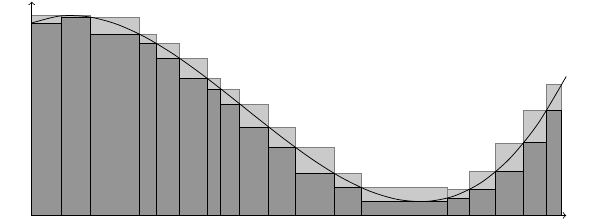
\includegraphics[scale=0.6]{diagrams/riemann}
%\begin{tikzpicture}[scale=2, domain=0:5]
%	\draw[<->] (0,2) -- (0,0) -- (5,0);
%	\draw[smooth,samples=20, domain=0.0:5.0] plot(\x, {(\x^3 - 6 * \x^2 + 4 * \x + 18)/10});
%\end{tikzpicture}
\end{figure}

Given an $n$-cube $[\![\boldsymbol{a}, \boldsymbol{b}]\!]$ we must cut each $[\![a_i, b_i]\!]$ into partitions.
Previously we used generalized partitions and did not mind if pieces overlapped or exceeded the original range.
However, for building our Riemann sums, we are only interested in partitions in the traditional, non-intersecting sense.

\begin{definition}
	Given an oriented interval $[\![a,b]\!]$ of the real line, we say that a partition of $[\![a,b]\!]$, $\{P_i\}_{i=1}^n$
	is an \textbf{interval partition of $\boldsymbol{[\![a,b]\!]}$} if its pieces are:
	\begin{enumerate}
		\item \emph{Oriented intervals}: $P_i$ is an oriented interval of the real line for all $i$.
		\item \emph{Disjoint}: $P_i \otimes P_j = \emptyset$ for all $i,j$
	\end{enumerate}
	We denote the set of all such partition as $\mathcal{P}[\![a,b]\!]$.
\end{definition}

This greatly restricts the types of partitions we have access to.
Every interval partition will be --- up to substitution of ``$]\!], (\!($'' in place of ``$)\!), [\![$'' --- of the form:
\begin{equation}
	\Big\{ \; [\![a,x_1)\!), \; [\![x_1, x_2)\!), \; [\![x_2, x_3)\!),\; \ldots,\; [\![x_{n-1}, b]\!] \; \Big\}
\end{equation}
where $x_i$ is a monotone sequence (that is, either non-increasing or non-decreasing).
This is not to say that $P_i = [\![x_{i-1}, x_i )\!)$ as the pieces of $P$ may not be given in this order.
Regardless of the ordering, we select partitions $P^j \in \mathcal{P}[\![a^j,b^j)\!)$ for each dimension of $[\![a,b)\!)$.
To build our mesh, we construct smaller $n$-cubes $I_{i_1, \ldots, i_n}$ using the Cartesian product of pieces:
\begin{equation}
	I_{i_1, \ldots, i_n} = i_1 \times \ldots \times i_n
\end{equation}
where each $i_j$ is taken from $P^j$.
We are now ready to construct Riemann sums.

\begin{definition}
	Given $P=\{ P_j \}_{j=1}^n$ where $P_j \in \mathcal{P}[\![a_j, b_j]\!]$,
	and $f:[\![\boldsymbol{a}, \boldsymbol{b}]\!] \to \mathcal{R}$ then we define a Riemann sum $f_P$ to be:
	\begin{equation}
		f_P = \sum_{i_1 \in P_1} \ldots \sum_{i_n \in P_n} f(x_{i_1, \ldots, i_n}) \text{vol}(I_{i_1, \ldots, i_n})
	\end{equation}
	where $x_{i_1, \ldots, i_n}$ is any point chosen from $I_{i_1, \ldots, i_n}$.
\end{definition}

Note that we specify \emph{a} Riemann sum, not \emph{the} Riemann sum.
There are several ways to choose $x_{i_1,\ldots,i_n} \in I_{i_1, \ldots, i_n}$ and different samplings can lead to different Riemann sums for the same partition and same function.
In $\mathbb{R}^1$, several common ways to sample include the left and right Riemann sums (which sample at the left and right boundaries), the trapezoidal Riemann sum (which averages the left and right) the upper Riemann sum (which samples at $\max(f(x_{i_1, \ldots, i_n}))$) and the lower Riemann sum (which samples at $\min(f(x_{i_1,\ldots,i_n}))$).

Recall our discussion of refinements from Chapter 2.
Given 2 partitions $P$ and $P'$ of the same set then we say $P \preceq P'$ if $P'$ is a refinement of $P$.
In this way we can induce a partial ordering on $\mathcal{P}[\![a,b]\!]$.
There is a unique smallest element in this partial ordering which is $[\![a,b]\!]$ itself; 
every partition by definition will refine $[\![a,b]\!]$.
Additionally, given $P,P' \in \mathcal{P}[\![a,b]\!]$ then propose that we can always find $Q$ that simultaneously refines both.
If $P=P'$ then trivially $Q=P$ is a common refinement.
Otherwise, we take:
\begin{equation}
	Q= [\![a,b]\!] \otimes \left( \bigoplus_{p\in P} \bigoplus_{p' \in P} p \otimes p' \right)
\end{equation}
The heavy lifting here is done by the fact that every point in $[\![a,b]\!]$ is covered by exactly one $p\in P$ and exactly one $p' \in P$.
The product of any two partition pieces will then be the smallest common interval with multiplicity 1.
Multiplying the entire thing by $[\![a,b]\!]$ is done to correct the sign.
As we go up in our ordering, our mesh becomes increasingly fine.
Taking the Riemann sum of the suprema of this poset gives us the Riemann integral.

\begin{definition}
The Riemann integral of a function $f:\mathbb{R}^n \to \mathbb{R}$ over a $k$-cube $[\![\boldsymbol{a}, \boldsymbol{b}]\!]$
where $P = \sup \Big\{ \mathcal{P} [\![a,b]\!] \Big\}$
	\begin{equation}
		\int_{[\![a,b]\!]} f(x) \; dx = f_P
	\end{equation} 
	We say that a function is \textbf{Riemann integrable} if the upper and lower Riemann sums converge.
\end{definition}

\todo[inline]{redo for arbitrary generalized partition with pieces going to zero}

%%%%%%%%%%%%%%%%%%%%%%%%%%%%%%%%%%%%%%%%%
% DIFFERENTIAL FORMS
%%%%%%%%%%%%%%%%%%%%%%%%%%%%%%%%%%%%%%%%%

\subsection{Differential Forms}

Rather than thinking of integrals as functions over $n$-rectangles, an often more useful language is to use 
\emph{differential forms}.
We define a \textbf{(differential) 0-form} $\beta$ on $\mathbb{R}^n$ as any function 
$\beta : \mathbb{R}^n \to \mathbb{R}$.
And there is very little else to say as they are just functions on $\mathbb{R}^n$.



A \textbf{(differental) 1-form} $\omega$ on $\mathbb{R}^n$ is an expression of the form:
\begin{equation}
	\omega = f_1(\text{x}) \; dx_1 + f_2(\text{x}) \; dx_2 + \ldots + f_n(\text{x}) \; dx_n
\end{equation}
Now this look very much like something we're used to integrating.
Specifically it is something that be used as an integrand over a 1 dimensional domain.
For example, Green's theorem is introduced using differential forms without even mentioning them as such.
\begin{equation}
	\tag{Green's Theorem}
	\textcolor{black!40}{
		\int_D \left( \frac{\partial f_2}{\partial x} - \frac{\partial f_1}{\partial y}  \right) \;dx\;dy 
		=\int_{C}
	} f_1(x,y) \; dx + f_2(x,y) \; dy
\end{equation}
Here $C$ is a closed curve that encloses $D$ a region in the $(x,y)$ plane; hence the right-hand side is an integral of
a 1-form over a 1-dimensional curve.
Having multiple $dx_i$ appearing in a single integrand may initially seem unusual when first presented, 
but is quite intuitively handled.
Integration is linear so just as we can separate $\int f(x) + g(x) dx$ into $\int f(x) dx + \int g(x) dx$, we can similarly break
up an integral of a 1-form into the sum of integrals over \emph{basic} 1-forms (1-forms involving a single term).
\begin{equation}
	\int f_1(\text{x}) \; dx_1 + f_2(\text{x}) \; dx_2 + \ldots + f_n(\text{x}) \; dx_n
	=
	\sum_{i=1}^n \left( \int f_i \; dx_i \right)
\end{equation}


Adding two 1-forms then is quite straight-forward; simply collect terms with matching $dx_i$.
So if we can add differential forms but what about multiplication?
For a 0-form $\beta$ and 1-form $\omega$ as defined above, the answer the answer is a simple yes:
\begin{equation}
	(\beta \cdot \omega)(\text{x}) = \beta(\text{x})f_1(\text{x})dx_1 + \ldots  + \beta(\text{x})f_n(\text{x})dx_n
\end{equation}
The result is a 1-form where each basic 1-form term is the product of $f_i$ and $\beta$ in $\mathbb{R}$.
To ``multiply'' two 1-forms together however we must turn instead to the wedge product $\wedge$.

First of all, the wedge product is primarily defined by being \emph{anti-commutative} or \emph{skew-symmetric}.
That is, $dx \wedge dy = -dy \wedge dx$ and several results will immediately follow.
When applied to two identical $dx$, we have $dx \wedge dx = - dx \wedge dx$ and so $dx \wedge dx = 0$.
Additionally, for any permutation $\sigma$ of $[p]$
\begin{equation}
	dx_1 \wedge ... \wedge dx_p = \text{sgn}(\sigma) \; dx_{\sigma(1)} \wedge ... \wedge dx_{\sigma(p)}
\end{equation}
The wedge product of two 1-forms moves us out of the realm of 1-forms which have basis $dx_i$ and into the 
realm of 2-forms with basis $dx_i \wedge dx_j$.


\begin{definition}
	Given a $k$-rectangle $\Omega \in \mathbb{R}^n$ with coordinates $\text{x} = (x_1, x_2, \ldots, x_n)$
	A \textbf{differential $p$-form} $\beta$ over $\Omega$ has the form:
	\begin{equation}
		\beta = \sum_{j_1 \in [n]} \ldots \sum_{j_p \in [n]} b_{(j_1, \ldots, j_p)}(\text{x}) \; 
				\text{d} x_{j_1} \wedge \ldots \wedge \text{d} x_{j_p}
	\end{equation}
	Typically, we will take $j$ to be the vector $(j_1, \ldots, j_p)$ and express $\beta$ instead as a single sum multi-indexed
	by $j$, $\sum_j b_j(x) \; dx_{j_1} \wedge \ldots \wedge dx_{j_p}$.
	We denote the space of all $p$-forms on $\Omega$ by $\Lambda^p(\Omega)$.
\end{definition}


\begin{definition}
	Let $\alpha = \sum_i a_i(x) \; dx_{i_1} \wedge \ldots \wedge dx_{i_p} \in \Lambda^p(\Omega)$ and 
	$\beta = \sum_j b_j(x) \; dx_{j_1} \wedge \ldots \wedge dx_{j_q} \in \Lambda^q(\Omega)$. We extend the
	wedge product $\wedge : \Lambda^p(\Omega) \times \Lambda^q(\Omega) \to \Lambda^{p+q}(\Omega)$ by:
	\begin{equation}
		\alpha \wedge \beta  = \sum_{i,j} a_i(x) b_j(x) \; 
			dx_{i_1} \wedge \ldots \wedge dx_{i_p} \wedge 
			dx_{j_1} \wedge \ldots \wedge dx_{j_q}
	\end{equation}
\end{definition}

Although we take all possible $\binom{n}{q} \cdot \binom{n}{p}$ pairs of 
$a_i (x) dx_{i_1} \wedge \ldots \wedge dx_{i_p}$ and $b_i (x) dx_{i_1} \wedge \ldots \wedge dx_{i_p}$,
most of the possible terms will end up being zero.
If \emph{any} of the terms in $dx_{i}$ appears in $dx_{j}$, then the wedge product will be zero 
and no term will be contributed.
As such, if $q+p > n$, there will be a duplicate in every term and so the entire sum will be zero.
When all is said and done, at most we will have $\binom{n}{p+q}$ terms.
Rather than the skew-symmetry we had when commuting $dx \wedge dy$, in higher dimensions the sign depends on 
$p \cdot q$ of the $p$-form and $q$-form we are commuting.
Specifically, 
\begin{equation}
	\alpha \wedge \beta = (-1)^{pq} \beta \wedge \alpha
\end{equation}
This can be easily seen by commuting each of $dx_{j_1}, \ldots dx_{j_q}$ terms each past 
$dx_{i_1}\wedge \ldots \wedge dx_{i_p}$. 
So we are commuting $q$ terms each past $p$ terms, reversing the sign each time for a net $(-1)^{pq}$.


The wedge product is only one part of our algebra of differential forms.
We have several other nice identities for its behaviour with addition and multiplication.
For the following, we consider $f$ to be a function on $\mathbb{R}^n$.
Additionally we consider the differential forms $\omega_1$ and $\omega_2$ to be $k$-forms, $\alpha$ to be a $p$-form
 and $\beta$ to be an $q$-form.
Then we have the following:
\begin{align}
	(\omega_1 + \omega_2) \wedge \alpha  & \;=\; \omega_1 \wedge \alpha + \omega_2 \wedge \alpha \\
	(\omega_1 \wedge \alpha) \wedge \beta & \;=\; \omega_1 \wedge ( \alpha \wedge \beta ) \\
	(f \cdot \omega_1) \wedge \alpha & \;=\;  f \cdot (\omega_1 \wedge \alpha) \;=\; \omega_1 \wedge (f \cdot \alpha)
\end{align}
These should all be quite obvious from definitions. 
We should also note the identities which are \emph{not} present.
We have defined the sum of $\omega_1$ and $\omega_2$: two differential forms which are the same dimension but not
the sum of $\alpha$ and $\beta$: differential forms with different dimension.
It is clear how one would add two differential forms of the same dimension as both were defined as sums to begin with.
We also do not define the multiplication of $\cdot$ two differential forms but we multiplying a form by a function is simply:
\begin{equation}
	(f \cdot \alpha) (x) = \sum_i f(x)\cdot a_i(x) \; dx_{i_1} \wedge \ldots \wedge dx_{i_p}
\end{equation}


Integrating over a $k$-form is quite simple.
First we shall consider integrating a $k$-form over a $k$-rectangle in $\mathbb{R}^k$.
Such a $k$-form is also known as a \emph{top-dimensional form}.
As we saw previously, any form of higher degree must be zero.
If $\omega$ is such a top form then we can always write
\begin{equation}
	\omega = f \; dx_1 \wedge \ldots \wedge dx_k
\end{equation}
for some function $f$.
Other presentations of $\omega$ exist, but we can always achieve such a presentation by commuting over $\wedge$ 
to the canonical ordering $x_1, \ldots, x_n$.
Once we have the $k$-form in this presentation, we just remove the wedges and evaluate the integral using the
integrand $f \; dx_1 \;dx_2 \ldots dx_k$.

\begin{definition}
Let $\alpha$ be a $k$-form on $\Omega \subset \mathbb{R}^n$ of the form $\alpha = A(x) \; \text{d}x_1 \wedge ... \wedge \text{d} x_n$.
If $A \in \mathcal{L}^1 (\Omega , \text{d}x)$ then we define:
\begin{equation}
\int_\Omega \alpha = \int_\Omega A(x) \; \text{d}x
\end{equation}
Where the left-hand side is the integral of a $k$-form and the right-hand side is a Lebesgue integral.
For any $\beta \in \Lambda^k (\Omega)$ we extend this definition linearly as the sum of integrals.
\end{definition}

\begin{definition}
Exterior derivative
\end{definition}

\todo[inline]{...}

\begin{equation}
d(\alpha \wedge \beta) = (d \alpha) \wedge \beta + (-1)^j \alpha \wedge ( d \beta)
\end{equation}


%%%%%%%%%%%%%%%%%%%%%%%%%%%%%%%%%%%%%%%%%
% SINGULAR CUBE
%%%%%%%%%%%%%%%%%%%%%%%%%%%%%%%%%%%%%%%%%
\subsection{Singular Cubes}

Up until now we have been dealing with the very small set of axis aligned $k$-rectangles 
which is a very limiting class to be restricted to.
Instead we would like to be able to integrate over $k$-rectangles that are deformed by some smooth function.
So assume that we have $X \subset \mathbb{R}^m$ and $Y \subset \mathbb{R}^n$ and a smooth map 
 $\varPhi : X \to Y$.
Not only can we map points from $X$ to points in $Y$ but we can \emph{push foward} vectors from $X$ to vectors in $Y$
and with them, push forward tangent spaces as well.


\begin{definition}
	We denote the \textbf{standard $\boldsymbol{k}$-cube} as the specific $k$-rectangle $[\![0,1]\!]^k$ in 	
	$\mathbb{R}^n$ which is the Cartesian product of $k$ copies of $[\![0,1]\!]$.
	We also consider $[\![0,1]\!]^0 = \{0\}$.
	Given an $n$-dimensional manifold $M$, a \textbf{singular $\boldsymbol{k}$-cube in $\boldsymbol{M}$} is a 
	smooth differentiable map $c$ from the standard $k$-cube to $M$, $c:[\![0,1]\!]^k$
	\todo[inline]{Singular $k$-cube: differentiable map $c$ from standard $k$-cube to $k$-dimensional manifold.}
\end{definition}


It is a common abuse of notation to use $c$ to also to refer to the image $c( [\![ 0,1]\!]^k ) \subseteq M$.
The choice of using specifically the standard $k$-cube is arbitrary.
A differentiable map $f$ from $[\![a,b]\!]$ can always be composed with $g:t \mapsto ta +(1-t)b$ 
to get singular cube $c=f \circ g$.
Gives us innumerably more shapes to work with.
Hemisphere for example is the singular 2-cube given by $(r, \varphi) \to r \cos(\pi \varphi) x+ r \sin(\pi \varphi) y$


However if we have a valid integral $\int_{\Omega} \omega$ with $\Omega$ in some space $X$, 
if we push forward $\Omega$ by some function $c$ to another space $Y$, 
then the integral $\int_{c(\Omega)} \omega$ is no longer valid.
The differential form $\omega$ was expressed in coordinates for $X$ but now that the domain of the integral is in $Y$,
we must perform a change of coordinates.
The true reason why we use differential forms is how cleanly they handle this change in coordinates 
through the use of pull-backs.

Informally, a pullback is a \emph{reversed} function composition.
In typical function composition $(f \circ g)(x) = f(g(x))$, for input $x$ one first evaluates the second function $g$ at $x$
before feeding the result of $g(x)$ into the first function $f$.
The pre-composition or pullback would be $f^*g = g(f(x))$. 
One first evaluates the first function and feeds the result into the second.
Gets its name from pulling $f$ back through $g$.


\todo[inline]{pullbacks and forms}

\begin{equation}
F^* (\alpha \wedge \beta ) = (F^* \alpha) \wedge (F^* \beta)
\end{equation}

\begin{equation}
F^* (d \beta ) = dF^* \beta
\end{equation}

\todo[inline]{vbox}


If we again have $\beta = \sum_j b_j(\text{x}) dx_{j_1} \wedge \ldots \wedge dx_{j_k} \in \Lambda^k(\Omega)$
and some \todo{smooth + differentiable?} map $F: X \to \Omega$.
The pull-back of $\beta$ is
\begin{equation}
F^* \beta = \sum_j  b_j ( F(x)) (F^* \text{d}x_{j_1}) \wedge ... \wedge (F^* \text{d} x_{j_k})
\end{equation}
and
\begin{equation}
F^* \text{d}x_j = \sum_\ell \frac{\partial F^j}{\partial x_\ell} \; \text{d} x_\ell
\end{equation}

Which can be reduced by:
\begin{align}
F^ * \beta & = \sum_j  b_j ( F(x)) (F^* \text{d}x_{j_1}) \wedge ... \wedge (F^* \text{d} x_{j_k}) \\
& = \sum_j  b_j ( F(x))  
\left( \sum_\ell \frac{\partial F^{j_1}}{\partial x_\ell} \; \text{d} x_\ell \right)
\wedge ... \wedge  
\left( \sum_\ell \frac{\partial F^{j_k}}{\partial x_\ell} \; \text{d} x_\ell \right) \\
& = \sum_j b_j ( F(x)) \; \text{det}\left( J_F \right) \; \text{d}x_{j_1} \wedge ... \wedge \text{d} x_{j_k}
\end{align}

Which is significant given the change of variable formula for integration:

\begin{equation}
\int_{\phi(U)} \! f(v) \; dv = \int_U \! f(\phi(u)) \; |\text{det}\phi'(u)| \; du
\end{equation}

\begin{theorem}
Let $F : X  \to \Omega$ be an (orientation-preserving diffeomorphism) and $\alpha$ an integrable $n$-form on $\Omega$ then
\begin{equation}
\int_{F(X)} \alpha = \int_X F^* \alpha
\end{equation}
\end{theorem}




To integrate over a manifold $M$, we first observe that each local chart in the manifold is essentially a singular cube.
If the chart is not a map over the standard cube, then there exists a diffeomorphism 
that can be composed with the local map to transform it into a singular cube.
It is then a matter of stitching together these local charts so that points in the manifold are not ``double-counted''.
To do this we use a partition of unity on $M$: a collection of functions $\theta_k \geq 0$ such that 
for all points in $x \in M$, $\sum_k \theta_k(x) = 1$.
In addition we also enforce that for each function $\text{supp} \theta_k$ and that at each point in $M$, there are only
a finite number of functions such that $\theta_k \neq 0$.

$\{ \psi_i \}$ a partition of unity with locally finite cover $\{ U_i, \psi_i \}$ of consistently oriented coordinate charts.

\begin{equation}
\int_M \alpha = \sum_i \int_{U_i} \psi_i \alpha
\end{equation}


%%%%%%%%%%%%%%%%%%%%%%%%%%%%%%%%%%%%%%%%%
%
% STOKES' THEOREM
%
%%%%%%%%%%%%%%%%%%%%%%%%%%%%%%%%%%%%%%%%%
\section{Stokes' Theorem}

When discussing differential forms an equation called \emph{Green's Theorem} was shown. 
Green's Theorem allows for one to convert between an integral over a 2-dimensional region and a 1-dimensional integral
over a curve that bounds it.
This turns out to be just one instance of the more general \emph{Stokes' Theorem} 
which will work in higher dimensions as well.
To do so we will first need to generalize the notion of a bounding region or boundary.



%%%%%%%%%%%%%%%%%%%%%%%%%%%%%%%%%%%%%%%%%
% BOUNDARY
%%%%%%%%%%%%%%%%%%%%%%%%%%%%%%%%%%%%%%%%%
\subsection{Boundary Operator}


In one dimension, the boundary of an interval was quite straight-forward.
For a positively oriented interval, the boundary was composed of two points; 
the right end-point was positive and the left end-point was negative.
From the perspective of $k$-rectangles, 
the $\partial$ operator has mapped an oriented 1-rectangle to a set of oriented 0-rectangles.
We will now generalize the boundary to map an oriented $n$-rectangle to an $(n-1)$-rectangle.


\begin{definition}
	Let  $[\![\boldsymbol{a}, \boldsymbol{b}]\!]$ be a a $k$-rectangle in $\mathbb{R}^n$.
	Additionally, let $i_1, i_2, \ldots, i_k$ be the unique non-decreasing sequence of indices such that $a_{i_j} \neq b_{i_j}$.
	The \textbf{boundary of $ \boldsymbol{[\![ a,b ]\!]} $ }, denoted the operator $\partial$ is given by
	\begin{align}
		\partial \left( [\![ \boldsymbol{a}, \boldsymbol{b} ]\!] \right) 
		= \bigoplus_{j=1}^k (-1)^j \;
			\left(	
				[\![ 	(\boldsymbol{a}^{[\![1,n]\!]}), 
					\;\;\;
					(\boldsymbol{b}^{[\![1,i_j)\!)} 
						\oplus \boldsymbol{a}^{\hset{i_j}}
						\oplus \boldsymbol{b}^{(\!(i_j,n]\!]}) 
				]\!] \right.\;
			\notag\\
			\ominus \left.
				[\![ 	(\boldsymbol{a}^{[\![1,i_j)\!)}
						\oplus \boldsymbol{b}^{\hset{i_j}}
						\oplus \boldsymbol{a}^{(\!(i_j, n]\!]}), 
					\;\;\;		 
					(\boldsymbol{b}^{[\![1,i_j)\!)}) 			
				]\!]
			\right)
	\end{align}
\end{definition}


The above equation will require a bit of unpacking to digest featuring oriented intervals in two different contexts.
The first appears in the superscripts of $\boldsymbol{a}$ and $\boldsymbol{b}$. 
The intervals $[\![1, i_j)\!)$ and $(\!(i_j, n]\!]$ are  and is an interval over vector indices just as in Chapter 3.
Thus, the term $\boldsymbol{a}^{[\![1,i_j)\!)}$ refers to the vector $(a_1, a_2, \ldots, a_{i_j-1})$ 
while the term $\boldsymbol{b}^{(\!(i_j,n]\!]}$ refers to $(b_{i_j+1}, b_{i_j+2}, \ldots, b_{n})$.
This provides a compact notation to partition the original range of indices into 3 pieces: $[\![ 1,i_j )\!)$, $\hset{i_j}$, and $(\!(i_j, n]\!]$.
Formally, we are actually using the hybrid sets $\hset{(i_j)^1}$ but we omit multiplicity of one (and will continue to do so through out the section) to lighten notation.


Next we use the pointwise sum $\oplus$ we reconstruct $n$-dimensional vectors from our pieces.
We then construct a $(k-1)$-rectangle using these vectors as in (4.8).
Hence we will have terms of the forms:
\begin{align}
	[\![a_1, b_1]\!]
	\times \ldots \times
	[\![a_{i_{j-1}}, b_{i_{j-1}}]\!]
	\times
	[\![a_{i_j}, a_{i_j}]\!]
	\times
	[\![a_{i_{j-1}}, b_{i_{j-1}}]\!]
	\times \ldots \times
	[\![a_n, b_n]\!]
	\\
	[\![a_1, b_1]\!]
	\times \ldots \times
	[\![a_{i_{j-1}}, b_{i_{j-1}}]\!]
	\times
	[\![b_{i_j}, b_{i_j}]\!]
	\times
	[\![a_{i_{j-1}}, b_{i_{j-1}}]\!]
	\times \ldots \times
	[\![a_n, b_n]\!]
\end{align}


In each Cartesian product, the terms at $i_j$: $[\![a_{i_j}, a_{i_j}]\!]$ and $[\![b_{i_j}, b_{i_j}]\!]$ are both 0-cubes.
Since we defined the sequence $i_j$ by $a_{i_j} \neq b_{i_j}$, 
these 0-rectangles are replacing 1-cubes in $[\![\boldsymbol{a}, \boldsymbol{b}]\!]$.
Hence we are indeed left with a $(k-1)$-cube.




%%%%%%%%%%%%%%%%%%%%%%%%%%%%%%%%%%%%%%%%%
% BOUNDARY OF A 1-RECTANGLE
%%%%%%%%%%%%%%%%%%%%%%%%%%%%%%%%%%%%%%%%%
\subsection{Example: \emph{Boundary of a 1-rectangle}}
Let $\boldsymbol{a}= (a_1)$ and $\boldsymbol{b} = (b_1)$ be trivial 1-tuples. 
Then $[\![\boldsymbol{a}, \boldsymbol{b}]\!] = [\![a_1, b_1]\!]$
It follows that:
\begin{align*}
	\partial ( \; [\![ \boldsymbol{a}, \boldsymbol{b} ]\!] \; )
	=& \; (-1)^i ( [\![\boldsymbol{a}^{[\![1,1)\!)}, \boldsymbol{b}^{[\![1,1)\!)} ]\!]
	\times \hset{a_1} \times
	[\![\boldsymbol{a}^{(\!(1,1]\!]}, \boldsymbol{b}^{(\!(1,1]\!]} ]\!]\\
	&\; \ominus
	[\![\boldsymbol{a}^{[\![1,1)\!)}, \boldsymbol{b}^{[\![1,1)\!)} ]\!]
	\times \hset{b_1} \times
	[\![\boldsymbol{a}^{(\!(1,1]\!]}, \boldsymbol{b}^{(\!(1,1]\!]} ]\!] )\\
	=& \; \ominus [\![\boldsymbol{a}^{\emptyset}, \boldsymbol{b}^{\emptyset} ]\!]
	\times \hset{a_1} \times
	[\![\boldsymbol{a}^{\emptyset}, \boldsymbol{b}^{\emptyset} ]\!]\\
	& \; \oplus
	[\![\boldsymbol{a}^{\emptyset}, \boldsymbol{b}^{\emptyset} ]\!]
	\times \hset{b_1} \times
	[\![\boldsymbol{a}^{\emptyset}, \boldsymbol{b}^{\emptyset} ]\!] \\
	=& \; \hset{b_1} \ominus \hset{a_1} \\
	=& \; \hset{a^{-1}, b^{1}}
\end{align*}

One may notice a relationship between this result and the fundamental theorem of calculus:
\begin{equation}
	\int_a^b F'(x) \; dx = F(b) - F(a)
\end{equation}
Which one could easily rewrite as $\int_{[\![a,b]\!]} F'(x) \; dx = \sum (\partial([\![a,b]\!]))$.
Indeed, this is why we have defined the boundary function as such, but more general statements await.
We defined the boundary for not just intervals on $\mathbb{R}$ but $k$-cubes in $\mathbb{R}^n$.




%%%%%%%%%%%%%%%%%%%%%%%%%%%%%%%%%%%%%%%%%
% BOUNDARY OF A 3-RECTANGLE
%%%%%%%%%%%%%%%%%%%%%%%%%%%%%%%%%%%%%%%%%
\subsection{Example: \emph{Boundary of a 3-rectangle}}
Let $\boldsymbol{a} = (0,0,0)$ and $\boldsymbol{b} = (1,1,1)$.
Omitting the intermediate step, we find the boundary of $[\![ \boldsymbol{a}, \boldsymbol{b} ]\!]$ to be:
\begin{align*}
	\partial ( \; [\![ \boldsymbol{a} , \boldsymbol{b} ]\!] \; ) =
	& 	\; \ominus \; \left( \hset{0} \times [\![0,1]\!] \times [\![0,1]\!] \right)
		\; \oplus \; \left( \hset{1} \times [\![0,1]\!] \times [\![0,1]\!] \right)
	\\& 	\; \oplus \; \left( [\![0,1]\!] \times \hset{0} \times [\![0,1]\!] \right)
	 	\; \ominus \; \left( [\![0,1]\!] \times \hset{1} \times [\![0,1]\!] \right)
	\\& 	\; \ominus \; \left( [\![0,1]\!] \times [\![0,1]\!] \times \hset{0} \right)
	  	\; \oplus \; \left( [\![0,1]\!] \times [\![0,1]\!] \times \hset{1} \right)
\end{align*}

This may not be the most enlightening expression on its own.
In Figure 4.3 below, the 3-rectangle given by $[\![\boldsymbol{a}, \boldsymbol{b}]\!]$ can be seen as a cube in three dimensions.
Physically, the 3-rectangle is a solid cube and includes all interior points.
The boundary meanwhile are just the rectangular outer faces, which conveniently,
 there are also six to match the six terms of $\partial[\![\boldsymbol{a},\boldsymbol{b}]\!]$.

\begin{figure}[ht]
\caption[Unit cube with boundary]{The unit cube in $\mathbb{R}^3$ with positive orientation can be represented as the 3-rectangle: $[\![(0,0,0), (1,1,1) ]\!]$ is shown as a wire-frame. 
The six faces that make up its boundary are shaded and labeled with their corresponding terms.
%Now with 100% more right-handed
}
\centering
\begin{tikzpicture}[y=1.4cm, x=2.8cm]	
 	%axis
 	
 	%left
	\draw[color=black, dashed, <-] (0.35, 1.35) --++ (-0.7, 0) node[anchor=east, black] {$\ominus \hset{0} \times [\![0,1]\!] \times [\![0,1]\!]$};
	%back
	\draw[color=black, dashed, <-] (1.2,1.7) --++ (1,1) node[anchor=west, black] {$\ominus \; [\![0,1]\!] \times \hset{1} \times [\![0,1]\!]$};
	%bottom
	\draw[color=black, dashed, <-] (0.85,0.35) --++ (0,-1) node[anchor=north, black] {$\ominus \; [\![0,1]\!] \times [\![0,1]\!] \times \hset{0}$};
 	
 	\filldraw[fill=black!20] (0,-0.2) --++ (1,0) --++ (0.7,0.7) --++ (-1,0) --++ (-0.7,-0.7);
	\filldraw[fill=black!20] (0.77,0.77) --++ (1,0) --++ (0,2) --++ (-1,0) --++ (0, -2);
	\filldraw[fill=black!20] (-0.1,0) --++ (0,2) --++ (0.7,0.7) --++ (0,-2) --++ (-0.7,-0.7);
 	
	\draw[->] (-1,0) -- coordinate (x axis mid) (3,0) node[anchor=north] {$x$};
    	\draw[->] (0,-1) -- coordinate (y axis mid) (0,4) node[anchor=east] {$z$};
	\draw[->] (-0.7,-0.7) node[anchor=north] {$y$} --++ (2.7,2.7) ;
	
	\draw[very thick] (0,0) --++ (1,0) --++ (0.7,0.7) --++ (-1,0) --++ (-0.7,-0.7);
	\draw[very thick] (0.7,0.7) --++ (1,0) --++ (0,2) --++ (-1,0) --++ (0, -2);
	\draw[very thick] (0,0) --++ (0,2) --++ (0.7,0.7) --++ (0,-2) --++ (-0.7,-0.7);
	\draw[very thick] (0,2) --++ (1,0) --++ (0.7,0.7) --++ (-1,0) --++ (-0.7,-0.7);
	\draw[very thick] (0,0) --++ (1,0) --++ (0,2) --++ (-1,0) --++ (0, -2);
	\draw[very thick] (1,0) --++ (0,2) --++ (0.7,0.7) --++ (0,-2) --++ (-0.7,-0.7);
	
	\filldraw[fill=black!40] (0,2.2) --++ (1,0) --++ (0.7,0.7) --++ (-1,0) --++ (-0.7,-0.7);
	\filldraw[fill=black!40] (-0.07,-0.07) --++ (1,0) --++ (0,2) --++ (-1,0) --++ (0, -2);
	\filldraw[fill=black!40] (1.1,0) --++ (0,2) --++ (0.7,0.7) --++ (0,-2) --++ (-0.7,-0.7);

	%right
	\draw[color=black, dashed, <-] (1.35+0.1, 1.35) --++ (0.7, 0) node[anchor=west, black] {$\hset{1} \times [\![0,1]\!] \times [\![0,1]\!]$};
	%front
	\draw[color=black, dashed, <-] (0.5-0.07,1-0.07) --++ (-0.7,-0.7) node[anchor=east, black] {$[\![0,1]\!] \times \hset{0} \times [\![0,1]\!]$};
	%top
	\draw[color=black, dashed, <-] (0.85,2.35+0.2) --++ (0,1) node[anchor=south, black] {$[\![0,1]\!] \times [\![0,1]\!] \times \hset{1}$};
\end{tikzpicture}
\end{figure}

There are several ways to interpret and visualize the $\oplus$ and $\ominus$ sign associated with each face.
Most naturally in $\mathbb{R}^3$ for 2-rectangles is to give each a front and back side with the sign determining which to use.
Alternatively, a 2-rectangle has a boundary formed by 1-rectangles which when drawn as arrows, will all meet head-to-tail.
This induces a clockwise or counter-clockwise cycle around the edge of the rectangle and so $\circlearrowright$ and $\circlearrowleft$ are also commonly used.
This can be seen in Figure 4.4.
One may even notice that the normals produced by both are the same and choose to use that.
These are all conceptual tools, which are convenient to use particularly in $\mathbb{R}^2$ and $\mathbb{R}^3$.
There may not be such a nice physical interpretation in other spaces.


\begin{figure}[ht]
\caption[Orientations of 2-rectangles]{One way of visualizing the orientation of 2-rectangles using clockwise and counter-clockwise cycles of arrows for 1-rectangles. 
The boundary of $[\![a,b]\!] \times [\![c,d]\!]$ becomes the cycle: 
$(a,c) \to (b,c) \to (b,d) \to (a,d) \to (a,c)$.
Showing the relationship between $[\![a,b]\!] \times [\![c,d]\!]$ and $[\![b,a]\!] \times [\![d,c]\!]$ }
\centering
\begin{tikzpicture}

	\def\rectCycle#1#2#3#4{
		\draw[thick, ->, color=black!80] (#1,#2) -- (#3,#2);
		\draw[thick, ->, color=black!60] (#3,#2) -- (#3,#4);
		\draw[thick, ->, color=black!40] (#3, #4) -- (#1,#4);
		\draw[thick, ->, color=black!20] (#1,#4) -- (#1,#2);
		\draw[thick, ->] (#1, 0) -- (#3, 0);
		%\draw[fill] (#1,#2) circle (1 pt);
	}

	
	\rectCycle {0+1}{1} {0+2}{2};
	\draw[<->] (0,3) -- (0,0) -- (3,0);
	\draw[very thick, ->] (0,1) -- (0,2);
	\draw (0,1.5) node[anchor=east] {$+$};
	\draw (1.5,0) node[anchor=north] {$+$};
	%\draw (1.5, 1.5) node {$+$};
	\draw(1.5,1.5) node {$\;\circlearrowleft^+$};
	
	  
	\rectCycle {4+2}{1} {4+1}{2};
	\draw[<->] (4+0,3) -- (4+0,0) -- (4+3,0);
	\draw[very thick, ->] (4+0,1) -- (4+0,2);
	\draw (4+0,1.5) node[anchor=east] {$+$};
	\draw (4+1.5,0) node[anchor=north] {$-$};
	%\draw (4+1.5, 1.5) node {$-$};
	\draw(4+1.5,1.5) node {$\;\circlearrowright^-$};
	
	
	\rectCycle {8+2}{2} {8+1}{1};
	\draw[<->] (8+0,3) -- (8+0,0) -- (8+3,0);
	\draw[very thick, ->] (8+0,2) -- (8+0,1);
	\draw (8+0,1.5) node[anchor=east] {$-$};
	\draw (8+1.5,0) node[anchor=north] {$-$};
	%\draw (8+1.5, 1.5) node {$+$};
	\draw(8+1.5,1.5) node {$\;\circlearrowleft^+$};
	
	
	\rectCycle {12+1}{2} {12+2}{1};
	\draw[<->] (12+0,3) -- (12+0,0) -- (12+3,0);
	\draw[very thick, ->] (12+0,2) -- (12+0,1);
	\draw (12+0,1.5) node[anchor=east] {$-$};
	\draw (12+1.5,0) node[anchor=north] {$+$};
	%\draw (12+1.5, 1.5) node {$-$};
	\draw(12+1.5,1.5) node {$\;\circlearrowright^-$};
	
\end{tikzpicture}
\end{figure}


%%%%%%%%%%%%%%%%%%%%%%%%%%%%%%%%%%%%%%%%%
%
% CHAINS
%
%%%%%%%%%%%%%%%%%%%%%%%%%%%%%%%%%%%%%%%%%
\subsection{Chains}

In fact, we have already seen $k$-chains without mentioning them explicitly.
The boundary of a $k$-cube was the sum $\oplus$, of $2k$ $(k-1)$ cubes.
Chains do not have to be boundaries however, any linear combination of $k$-cubes will do.


\begin{definition}
We denote the Abelian group of of all $k$-cubes in $X$ as $C_k(X)$ (omitting $X$ when obvious by context).
An element $c \in C_k$(X) is called a \textbf{$\boldsymbol{k}$-chain on $X$} and is of the form:
\begin{equation}
	c = \bigoplus_{c_i \in X} \lambda_i c_i
\end{equation}
with integer coefficients $\lambda_i$ and  $k$-cubes in $c_i$.
If coefficients $\lambda_i$ are $\pm 1$ and $c$ is \emph{locally finite} (i.e. each $c_i$ intersects with only finitely many $c_j$ that have non-zero coefficients) then we say that $c$ is a \textbf{domain of integration}.
\end{definition}
	
	
Since $k$-chains are just linear combinations of $k$-cubes, we naturally extend many of our definitions linearly as well.
The integral $\int_c f$ of a $k$-chain $c=\bigoplus_i \lambda_i c_i$ is defined as $\lambda_i \int_{c_i} f  + \lambda_2 \int_{c_2} f + \ldots$.
Doing the same for the boundary operator $\partial$ we have:
\begin{align*}
	&\partial_k: C_k \to C_{k-1} \\
	&\partial_k(c) = \bigoplus_{i=1}^k \lambda_i \partial_k(c_i)
\end{align*}
Elegantly, the boundary operator now maps $k$-chains to $(k-1)$-chains!
\begin{equation}
	\ldots \xleftarrow{\partial_{k-1}} C_{k-1} \xleftarrow{\partial_{k}} C_k \xleftarrow{\partial_{k+1}} C_{k+1} \xleftarrow{\partial_{k+2}} ...
\end{equation}
The most natural next question becomes \emph{``What does $\partial_{k-1}( \partial_k ( c ))$ look like?''}




%%%%%%%%%%%%%%%%%%%%%%%%%%%%%%%%%%%%%%%%%
% BOUNDARY OF A BOUNDARY
%%%%%%%%%%%%%%%%%%%%%%%%%%%%%%%%%%%%%%%%%
\subsection{Example: \emph{Boundary of a boundary (of a 2-cube)}}
Let $\boldsymbol{a} =(a_1,a_2)$ and $\boldsymbol{b}= (b_1,b_2)$.
We wish to compute $\partial_1 ( \partial_2 ( \; [\![\boldsymbol{a}, \boldsymbol{b} ]\!] \; ) )$
\begin{align}
	\partial_1 ( \partial_2 ( [\![ a_1 , b_1 ]\!] \times [\![a_2, b_2 ]\!] ) )
	=	& 	\; \ominus 	\partial_1( \hset{0} \times [\![0,1]\!]) 
			\; \oplus \; 	\partial_1(\hset{1} \times [\![0,1]\!]) \notag \\
		& 	\; \oplus 	\partial_1( [\![0,1]\!] \times \hset{0}) 
			\; \ominus \; \partial_1([\![0,1]\!] \times \hset{1}) \\
	=	& 	\ominus	( 	\ominus \hset{(0,0)} \oplus \hset{(0,1)} ) 
			\;\oplus\;(	\ominus \hset{(1,0)} \oplus \hset{(1,1)}) \notag \\
		& 	\oplus ( 		\ominus \hset{(0,0)} \oplus \hset{(1,0)} ) 
			\;\ominus\;(	\ominus \hset{(0,1)} \oplus \hset{(1,1)}) \\
	=	& \;\emptyset	
\end{align}


When moving from (4.21) to (4.22), in addition to applying $\partial_1$ we also simplify, $\hset{x} \times \hset{y} = \hset{ (x,y) }$.
The identity ``$\partial \partial = 0$'' is not unique to $2$-cubes but holds for higher dimensions as well.


\begin{figure}[ht]
\caption[Boundary of a boundary (of a 2-cube)]{The boundary of 2-cube gives a cycle of oriented edges. Taking the boundary of again, at each corner, the negative boundary of one edge will be canceled by the positive boundary of the preceding edge.}
\centering
	\begin{tikzpicture}
	
		\draw (1,2.5) node {$C_2$};
		\filldraw[fill=black!40] (0,0) rectangle (2,2);
		\draw (1,1) node {$\;\circlearrowleft^+$};
		
		\draw[very thick, ->] (2.5,2.5) --++ (0.5,0) node[anchor=south] {$\partial_2$} --++ (0.5,0);
		
		\draw (4+1,2.5) node {$C_1$};
		\draw[thick, ->] (4+0,0) --++ (2,0);
		\draw[thick, ->] (4+2,0) --++ (0,2);
		\draw[thick, ->] (4+2,2) --++ (-2,0);
		\draw[thick, ->] (4+0,2) --++ (0,-2);
		
		\draw[very thick, ->] (6.5,2.5) --++ (0.5,0) node[anchor=south] {$\partial_1$} --++ (0.5,0);
		
		\draw (8+1,2.5) node {$C_0$};
		\draw[dashed] (8+0,0) --++ (0,2) --++ (2,0) --++ (0,-2) --++ (-2,0);
		\fill (8,0) node[anchor=north] {$-$} node[anchor=east] {$+$} circle (2pt);
		\fill (8+2,0) node[anchor=west] {$-$} node[anchor=north] {$+$}  circle (2pt);
		\fill (8+2,2) node[anchor=south] {$-$} node[anchor=west] {$+$} circle (2pt);
		\fill (8,2) node[anchor=east] {$-$} node[anchor=south] {$+$} circle (2pt);
		
	\end{tikzpicture}
\end{figure}


Let $[\![\boldsymbol{a}, \boldsymbol{b}]\!]$ be a $k$-rectangle in $\mathbb{R}^n$.
Then we have:
\begin{align}
	\partial_k \partial_{k-1} \left( [\![ \boldsymbol{a}, \boldsymbol{b} ]\!] \right) 
	= \bigoplus_{j=1}^k (-1)^j 
		& \;  \left( \; \partial_{n-1} \left(	
			[\![ 	\boldsymbol{a}^{[\![1,n]\!]}, \;\;
				\boldsymbol{b}^{[\![1,i_j)\!)}
					\oplus \boldsymbol{a}^{[\![i_j]\!]}
					\oplus \boldsymbol{b}^{(\!(i_j,n]\!]} 
			]\!] 
		\right) \right. \notag\\[-1em]
		& \ominus \; \left. \! \partial_{n-1} \left(
			[\![ 	\boldsymbol{a}^{[\![1,i_j)\!)}
					\oplus \boldsymbol{b}^{[\![i_j]\!]}
					\oplus \boldsymbol{a}^{(\!(i_j,n]\!]} , \;\;
				\boldsymbol{b}^{[\![1,n]\!]}
			]\!] 
		\right)\right) \\[1em]
	= \bigoplus_{j=1}^k \bigoplus_{\ell=1}^{k-1} (-1)^{j+\ell}
		\;&
			[\![ 	(\boldsymbol{a}^{[\![1,n]\!]}), \;\;
				(\boldsymbol{b}^{[\![1,i_j)\!) \;\oplus\; (\!(i_j,i_{j,\ell})\!) \;\oplus\; (\!(i_{j,\ell},n]\!]}
					\oplus \boldsymbol{a}^{[\![i_j]\!] \;\oplus\; [\![i_{j,\ell}]\!]})
			]\!] \notag\\[-1em]
		\ominus \;&
			[\![ 	(\boldsymbol{a}^{[\![1,i_{j,\ell})\!) \;\oplus\; (\!(i_{j,\ell},n]\!]}
					\oplus \boldsymbol{b}^{[\![i_{j,\ell}]\!]}), \;\;
				(\boldsymbol{b}^{[\![1,i_j)\!) \;\oplus\; (\!(i_j,n]\!]}
					\oplus \boldsymbol{a}^{[\![i_j]\!]})
			]\!] \notag\\
		\ominus \; &
			[\![ 	(\boldsymbol{a}^{[\![1,i_j)\!) \;\oplus\; (\!(i_j,n]\!]}
					\oplus \boldsymbol{b}^{[\![i_j]\!]}), \;\;
				(\boldsymbol{b}^{[\![1,i_{j,\ell})\!) \;\oplus\; (\!(i_{j,\ell},n]\!]}
					\oplus \boldsymbol{a}^{[\![i_{j,\ell}]\!]})
			]\!] \notag\\
		\oplus \;&
			[\![ 	(\boldsymbol{a}^{[\![1,i_j)\!) \;\oplus\; (\!(i_j,i_{j,\ell})\!) \;\oplus\; (\!(i_{j,\ell},n]\!]}
					\oplus \boldsymbol{b}^{[\![i_j]\!] \;\oplus\; [\![i_{j,\ell}]\!]}), \;\;
				(\boldsymbol{b}^{[\![1,n]\!]})
			]\!] 
\end{align}
Note that we have $i_j$ and $i'_\ell$; after applying the first boundary operator, one dimension of the $k$-cube is degenerate.
Hence for each sequence: $\{i_j\}_{j=1}^k$ we construct $\{i_{j,\ell}\}_{\ell=1}^{k-1}$ given by:
\begin{equation}
	i_{j,1} , \ldots, i_{j,k-1} = i_1, \ldots, \widehat{i_j}, \ldots, i_k
\end{equation}
The double sum iterates over all pairs but $\oplus$ commutes so the $(k-2)$-cube with degenerate dimensions $[\![i_j]\!] \oplus [\![i_{j,\ell}]\!]$ will be iterated over twice. 
The sequences depend on one another so it is not as simple as simply swapping $\ell$ and $j$:
\begin{equation}
   [\![i_j]\!] \oplus [\![i_{j,\ell}]\!] =
     \begin{cases}
       [\![i_\ell]\!] \oplus [\![i_{\ell,j-1}]\!] & j > \ell \\
       [\![i_{\ell+1}]\!] \oplus [\![i_{\ell+1,j}]\!] & j \leq \ell
     \end{cases}
\end{equation}
So each term representing a $(k-2)$-cube will occur twice in the sum.
Once with the iteration $(j,\ell)$ and once with $(\ell, j-1)$ or $(\ell+1, j)$.
In either case, $(-1)^{j+\ell}$ is inverted meaning the two cubes will cancel.
Leaving us with the boundary of a boundary being empty.
By linearity this extends to all chains as well as the sum of empty sets is of course still empty.


\begin{definition}
	A \textbf{chain complex} is a sequence of Abelian groups $\ldots, A_2, A_1, A_0, A_{-1}, A_{-2}, \ldots$ \linebreak
	which are connected by homomorphisms $d_n:A_n \to A_{n-1}$ such that $d_n \circ d_{n+1} = 0$ for all $n$.
	Typically written out as:
	\begin{equation}
		\ldots 	\xleftarrow{d_{k-1}} A_{k-1} 
				\xleftarrow{d_{k}} A_k 
				\xleftarrow{d_{k+1}} A_{k+1} 
				\xleftarrow{d_{k+2}} \ldots
	\end{equation}
	A \textbf{cochain complex} is a sequence of Abelian groups $\ldots, A^{-2}, A^{-1}, A^0, A^{1}, A^{2}, \ldots$
	which are connected by homomorphisms $d^n:A^n \to A^{n+1}$ such that $d^n \circ d^{n-1} = 0$ for all $n$.
	Typically written out as:
	\begin{equation}
		\ldots 	\xrightarrow{d^{k-1}} A^{k-1} 
				\xrightarrow{d^{k}} A^k 
				\xrightarrow{d^{k+1}} A^{k+1} 
				\xrightarrow{d^{k+2}} \ldots
	\end{equation}
\end{definition}

$(C_\bullet, \partial_\bullet)$ is just one instance of a chain complex known as the \emph{``cubic homology''}.
In the next chapter we will look at the more general \emph{``cubic singular homology''}.
As well as the related cochain complex: the \emph{``De Rham cohomology''} and how the two relate.










%%%%%%%%%%%%%%%%%%%%%%%%%%%%%%%%%%%%%%%%%
%
% STOKE'S THEOREM
%
%%%%%%%%%%%%%%%%%%%%%%%%%%%%%%%%%%%%%%%%%
\subsection{Stokes' Theorem}

Now we come to the statement of the generalized Stokes' Theorem itself.

Given a $k-1$-form $\omega$ and $k$ chain $M$, ...

\begin{equation}
	\int_{\partial M} \omega = \int_M d\omega
\end{equation}


In one dimension this is the fundamental theorem of calculus.

In two, it is Green's Theorem and three the Kelvin-Stokes Theorem.


First we will consider Stokes theorem for the standard cube $I^k = [0,1]^k \subset \mathbb{R}^k$.
In the previous section we saw how cumbersome representing the faces in $\partial I^k$, could be.

We will denote the faces of $I^k$ by $I^k_{i=0}$ and $I^k_{i=1}$ for the $i$-th faces of $I^k$.
This allows us to rewrite:

\begin{equation}
	\partial (I^k) = \bigoplus_{i=1}^k (-1)^i \left( I^k_{i=0} \ominus I^k_{i=1} \right) 
\end{equation}

A $k-1$-form $\omega$ can be written as the sum
\begin{equation}
	\omega 
		= \sum_{i=1}^k \omega_i 
		= \sum_{i=1}^k f_i \; dx_1 \wedge \ldots \wedge \widehat{dx_i} \wedge  \ldots \wedge dx_k
\end{equation}
but since everything: the integrals, $d$ and $\partial$ are all linear, we can work using just one of these terms.
Assuming Stokes' theorem holds for $\omega_i$ then we immediately have it for $\omega$ as well:
\begin{align*}
	\int_{\partial\Omega} \omega 
	&= \int_{\partial \Omega} (\omega_1 + \ldots + \omega_k) \\
	&= \int_{\partial\Omega} \omega_1 + \ldots + \int_{\partial\Omega} \omega_k  \\
	&= \int_{\Omega} d\omega_1 + \ldots + \int_\Omega d\omega_k \\
	&= \int_\Omega (d\omega_1 + \ldots + d\omega_k)\\
	&= \int_\Omega d(\omega_1 + \ldots + \omega_k) = \int_\Omega d\omega
\end{align*}

To compute $d\omega$, we have for each term in the sum:
\begin{align*}
	d \left( f_i dx_1 \wedge \ldots \wedge \widehat{dx_i} \wedge  \ldots \wedge dx_k \right) 
 		&= df_i \wedge dx_1 \wedge \ldots \wedge \widehat{dx_i} \wedge  \ldots \wedge dx_k \\ 
 		&= \left( \sum_{j=1}^k \frac{\partial f_i}{\partial x_j} dx_j \right)
 			\wedge dx_1 \wedge \ldots \wedge \widehat{dx_i} \wedge  \ldots \wedge dx_k \\ 
\end{align*}
But for $j \neq i$, there will be a duplicate $dx_j$ term and this collision will cause the term to go to zero.
Hence only one term in the sum, $i=j$ will actually result in a non-zero term:
\begin{align*}
	d \left( f_i dx_1 \wedge \ldots \wedge \widehat{dx_i} \wedge  \ldots \wedge dx_k \right) 
 		&= \left(\frac{\partial f_i}{\partial x_i} dx_i \right)
 			\wedge dx_1 \wedge \ldots \wedge \hat{dx_i} \wedge  \ldots \wedge dx_k \\ 
		&= (-1)^{i-1} \frac{\partial f_i}{\partial x_i}
 			 dx_1 \wedge \ldots \wedge dx_k \\ 
\end{align*}


Since this is an integral over the canonical basis $\text{x} = (x_1, \ldots, x_k)$ we can remove the wedge products and
integrate as normal.
\begin{align*}
	\int_{[0,1]^k} d\omega_i
		=&\; (-1)^{i-1} \int_{[0,1]^k} \frac{\partial f_i}{\partial x_i}\; d(x_1, \ldots, x_k) \\
		=&\; (-1)^{i-1} \int_{[0,1]^{k-1}} \left( \int_0^1 \frac{\partial f_i}{\partial x_i} dx_i \right) 
			\;d(x_1, \ldots, \widehat{x_i}, \ldots, x_k)\\
		=&\; (-1)^{i-1}\left( \int_{[0,1]^{k-1}} f_i(x_1, \ldots, x_{i-1}, 1, x_{i+1}, \ldots, x_k)
			\;d(x_1, \ldots, \widehat{x_i}, \ldots, x_k) \right.\\
		&\;	- \left. \int_{[0,1]^{k-1}} f_i(x_1, \ldots, x_{i-1}, 0, x_{i+1}, \ldots, x_k)
			\;d(x_1, \ldots, \widehat{x_i}, \ldots, x_k) \right)
\end{align*}
The trick here being Fubini's Theorem allowing us to evaluate the iterated integral in whichever order we choose.
On the other side of the equality we have:
\begin{align*}
	\int_{\partial I^k} \omega_i
		&= \sum_{j=1}^k (-1)^j \int_{I^k_{j=0}} \omega_i - \int_{I^k_{j=1}} \omega_i
\end{align*}
but $I^k_{j=0}$ is just a $k-1$-rectangle embedded in $\mathbb{R}^k$ by the map:
\begin{equation*}
	(x_1, \ldots x_{k-1}) \mapsto (x_1, \ldots, x_{j-1}, 0, x_{j}, \ldots x_{k-1})
\end{equation*}
So we could alternatively think of $I^k_{j=0}: I^{k-1} \to I^k$ as just a change in coordinates:
\begin{align*}
	\int_{\partial I^k} \omega_i 
		=&\; \sum_{j=1}^k (-1)^j 
			\left(\int_{I^{k-1}} (I^k_{j=0})^*\omega_i - \int_{I^{k-1}} (I^k_{j=1})^* \omega_i \right) \\
		=&\; \sum_{j=1}^k (-1)^j 
			\left(\int_{I^{k-1}} f_i (x_1, \ldots, x_{i-1}, 0, x_{i+1}, \ldots, x_k)
				\;dx_1 \wedge \ldots \wedge \widehat{dx_i} \wedge  \ldots \wedge dx_k \right. \\
		&	\left. - \int_{I^{k-1}} f_i (x_1, \ldots, x_{i-1}, 1, x_{i+1}, \ldots, x_k)
				\;dx_1 \wedge \ldots \wedge \widehat{dx_i} \wedge  \ldots \wedge dx_k \right)\\
		=&\; (-1)^i \left(\int_{I^{k-1}} f_i (x_1, \ldots, x_{i-1}, 0, x_{i+1}, \ldots, x_k)
				\;d(x_1, \ldots,\widehat{x_i},  \ldots, x_k) \right. \\
		&	\left. - \int_{I^{k-1}} f_i (x_1, \ldots, x_{i-1}, 1, x_{i+1}, \ldots, x_k)
				\;d(x_1, \ldots,\widehat{x_i},  \ldots, x_k) \right)
\end{align*}



In the final step we observe that all terms in the sum for $i \neq j$ end up disappearing leaving us with just the term for
$i=j$.
Clearly, both sides of the equation are the same and so Stokes' theorem holds for the standard cube.
From here, the remaining cases build on one another are quite straight-forward.
For a singular cube $c$, we have:
\begin{align*}
	\int_{\partial c} \omega
		&= \int_{c (\partial ([0,1]^k))} \omega \\
		&= \int_{\partial( [0,1]^k)} c^* \omega \\
		&= \int_{[0,1]^k} dc^* \omega \\
		&= \int_{[0,1]^k} c^* d \omega \\
		&= \int_c d\omega
\end{align*}
And for a chain $C=a_1 c_1 + \ldots + a_n c_n$ made up of singular cubes:
\begin{align*}
	\int_C d\omega 
		&= \int_{a_1c_1 + \ldots + a_nc_n	} d\omega \\
		&= a_1 \int_{c_1} d\omega + \ldots + a_n \int_{c_n} d\omega \\
		&= a_1 \int_{\partial c_1} \omega + \ldots + a_n \int_{\partial c_n} \omega \\
		&= \int_{a_1 \partial c_1 + \ldots a_n \partial c_n} \omega \\
		&= \int{\partial ( a_1c_1 + \ldots + a_n c_n)} \omega \\
		&= \int_{\partial C} \omega
\end{align*}

And so we have Stokes' theorem on general chains.

\todo[inline]{vbox}
\todo[inline]{vbox}
\todo[inline]{vbox}
\todo[inline]{vbox}



\section{Applications}

Integrating with hybrid set domains does not enable any new techniques that were previously not possible.
Using differential forms or digging even deeper with pseudo-forms and densities on manifolds, 
one can generalize integration to a vast class of structures.
These will all generally come back to some numeric integration ``back-end'' as we saw with differential forms.
In the end, to compute an integral with differential forms we still need to convert the wedge product
$dx_1 \wedge \ldots \wedge dx_k$ into $d(x_1, \ldots x_k)$.
While there are many options; the Riemann and Lebesgue integrals being the most famous  a whole host of 
less widely known formulations exist \cite{bochner1933integration, darboux1896leccons, henstock1991general}.


Hybrid set integration does not enable anything new.
It does enable us to bring the useful abstraction of orientation on a set into the ``back-end'' of integration.

The following examples will primarily be an application of existing, well-known methods for computing integrals but 
translated into the language of hybrid sets.
\todo[inline]{Why is this a good thing?}


%%%%%%%%%%%%%%%%%%%%%%%%%%%%%%%%%%%%%%%%%
% ''HAVING YOUR CAKE AND EATING IT TOO'' EXAMPLE
%%%%%%%%%%%%%%%%%%%%%%%%%%%%%%%%%%%%%%%%%
\subsection{Example: \emph{Irrational numbers}}

A Lebesgue measurable hybrid set can now have an orientation like Riemann integral intervals and the power of Lebesgue integration

\begin{equation}
	\int_1^0 1 -\mathbb{I}_\mathbb{Q}(x)\; dx
\end{equation}


%%%%%%%%%%%%%%%%%%%%%%%%%%%%%%%%%%%%%%%%%
% MESH EXAMPLE
%%%%%%%%%%%%%%%%%%%%%%%%%%%%%%%%%%%%%%%%%
\subsection{Example: \emph{Integrating a mesh}}

\begin{equation}
	f(x,y) = \frac{\sin(x) \cos(y)}{\cos^2(x) + \sin^2(y)}
\end{equation}


\begin{figure}[ht]
	\caption[Mesh Diagram]{The function $f(x,y) = \frac{\sin(x) \cos(y)}{\cos^2(x) + \sin^2(y)}$}
	\centering
	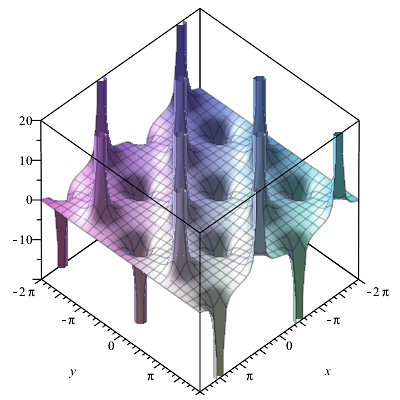
\includegraphics[scale=0.6]{diagrams/sinxcosy_cos2xsin2y.png}
\end{figure}

Anti-periodic $f(x+P) = -f(x)$


%%%%%%%%%%%%%%%%%%%%%%%%%%%%%%%%%%%%%%%%%
% CONTOUR EXAMPLE
%%%%%%%%%%%%%%%%%%%%%%%%%%%%%%%%%%%%%%%%%
\subsection{Example: \emph{Contour Integral}}








\chapter{Integration II}


%%%%%%%%%%%%%%%%%%%%%%%%%%%%%%%%%%%%%%%%%
%
% DIFFERENTIAL FORMS
%
%%%%%%%%%%%%%%%%%%%%%%%%%%%%%%%%%%%%%%%%%

\section{Differential Forms}

\begin{definition}
A $k$-form $\beta$ on the open set $\Omega \subset \mathbb{R}^n$ has the form:
\todo[inline]{open set or Lebesgue measurable sets??}
\begin{equation}
\beta = \sum_j b_j(x) \; \text{d} x_{j_1} \wedge ... \wedge \text{d} x_{j_k}
\end{equation}
where $j=(j_1, ..., j_k)$ is a $k$ dimensional multi-index. We say that $\beta \in \Lambda^k(\Omega)$
\end{definition}

We have not yet defined the $\wedge$ operator.

Anti-commutative: $\text{d} x \wedge \text{d} y = - \text{d}y \wedge \text{d} x$. 
Which implies for any permutation $\sigma$ of $\{1,...,k\}$:
\begin{equation}
dx_1 \wedge ... \wedge dx_k = \text{sgn}(\sigma) \; dx_{\sigma(1)} \wedge ... \wedge dx_{\sigma(k)}
\end{equation}

Anti-commutativity additionally implies that for all $x_i$, $dx_i \wedge dx_i = 0$. 

Let $\alpha = \sum_i a_i(x) \; dx_{i_1} \wedge ... \wedge dx_{i_\ell} \in \Lambda^\ell(\Omega)$ and
$\beta = \sum_j b_j(x) \; \text{d} x_{j_1} \wedge ... \wedge \text{d} x_{j_k} \in \Lambda^k(\Omega)$ then define:

\begin{equation}
\alpha \wedge \beta  := \sum_{i,j} a_i(x) b_j(x) \; dx_{i_1} \wedge ... \wedge dx_{i_\ell} \wedge dx_{j_1} \wedge ... \wedge dx_{j_k}
\end{equation}

Thus we can think of $\wedge$ as mapping a $k$-form and an $\ell$-form to a $(k+\ell)$-form, $\wedge : \Lambda^\ell(\Omega) \times \Lambda^k (\Omega) \to \Lambda^{k+\ell} (\Omega)$. By anti-commutativity we have:

\begin{equation}
\alpha \wedge \beta = (-1)^{k \ell} \beta \wedge \alpha
\end{equation}


\begin{definition}
Let $\alpha$ be a $k$-form on $\Omega \subset \mathbb{R}^n$ of the form $\alpha = A(x) \; \text{d}x_1 \wedge ... \wedge \text{d} x_n$.
If $A \in \mathcal{L}^1 (\Omega , \text{d}x)$ then we define:
\begin{equation}
\int_\Omega \alpha = \int_\Omega A(x) \; \text{d}x
\end{equation}
Where the left-hand side is the integral of a $k$-form and the right-hand side is a Lebesgue integral.
For any $\beta \in \Lambda^k (\Omega)$ we extend this definition linearly as the sum of integrals.
\end{definition}
\todo[inline]{Define $dx$ from $x_1 , ... , x_n$. Need to lift sign change from permutations}


\newpage
%%%%%%%%%%%%%%%%%%%%%%%%%%%%%%%%%%%%%%%%%
%
% PULL-BACKS (or coordinate changes)
%
%%%%%%%%%%%%%%%%%%%%%%%%%%%%%%%%%%%%%%%%%

\section{Pull-backs}

Benefit of differential forms is how cleanly they handle changes in coordinates.

\begin{definition}
$F: X \to \Omega$
Define the pullback $F^* \beta$
\begin{equation}
F^* \beta = \sum_j  b_j ( F(x)) (F^* \text{d}x_{j_1}) \wedge ... \wedge (F^* \text{d} x_{j_k})
\end{equation}
and
\begin{equation}
F^* \text{d}x_j = \sum_\ell \frac{\partial F^j}{\partial x_\ell} \; \text{d} x_\ell
\end{equation}
\end{definition}

Which can be reduced by:
\begin{align}
F^ * \beta & = \sum_j  b_j ( F(x)) (F^* \text{d}x_{j_1}) \wedge ... \wedge (F^* \text{d} x_{j_k}) \\
& = \sum_j  b_j ( F(x))  
\left( \sum_\ell \frac{\partial F^{j_1}}{\partial x_\ell} \; \text{d} x_\ell \right)
\wedge ... \wedge  
\left( \sum_\ell \frac{\partial F^{j_k}}{\partial x_\ell} \; \text{d} x_\ell \right) \\
& = ... \\
& = \sum_j b_j ( F(x)) \; \text{det}\left( J_F \right) \; \text{d}x_{j_1} \wedge ... \wedge \text{d} x_{j_k}
\end{align}

Which is significant given the change of variable formula for integration:

\begin{equation}
\int_{\phi(U)} \! f(v) \; dv = \int_U \! f(\phi(u)) \; |\text{det}\phi'(u)| \; du
\end{equation}

\begin{theorem}
Let $F : X  \to \Omega$ be an (orientation-preserving diffeomorphism) and $\alpha$ an integrable $n$-form on $\Omega$ then
\begin{equation}
\int_\Omega \alpha = \int_X F^* \alpha
\end{equation}
\end{theorem}

More algebra of differential forms

\begin{equation}
F^* (\alpha \wedge \beta ) = (F^* \alpha) \wedge (F^* \beta)
\end{equation}

\begin{definition}
Exterior derivative
\end{definition}

...

\begin{equation}
d(\alpha \wedge \beta) = (d \alpha) \wedge \beta + (-1)^j \alpha \wedge ( d \beta)
\end{equation}

...

\begin{equation}
F^* (d \beta ) = dF^* \beta
\end{equation}

\section{Integration over Manifolds}

\begin{example}
Integrate an atlas with overlapping charts (using inclusion-exclusion)
\end{example}
\newpage

\section{Stokes' Theorem}



\subsection{Example: \emph{Contour Integration}}
\todo[inline]{??????????}

Using Stokes' theorem and Inclusion/Exclusion to evaluate a tricky theorem like:

\begin{equation}
f(z) = \frac{z^2}{(z^2 + 2z + 2)}
\end{equation}

% http://en.wikipedia.org/wiki/Methods_of_contour_integration

 (2-3 pages)

\newpage

\chapter{Convolution}

Convolution is an operation which takes two functions and produces a third.
It takes one of the two input functions, and modifies one by mirroring and translating.
The resulting function is then the overlap between one of these functions as a function of the translation.
Visually, this can be seen below in Figure~\ref{fig:ConvolutionExample}.

+1 line

\begin{figure}[ht]
	\caption[Convolution of box signal with itself]{The convolution of the box signal 
	$f(t)=g(t)=\left( 0^\oiOpOp{-\infty,-0.5} \oplus 1^\oiClCl{-0.5,0.5} \oplus 0^\oiOpOp{0.5,\infty} \right)$ with itself.
	\emph{(from wikipedia; need to create new versions)}
	\label{fig:ConvolutionExample}}
	\centering
	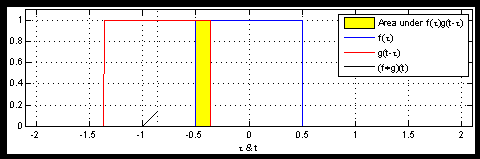
\includegraphics[scale=0.5]{diagrams/conv1}
	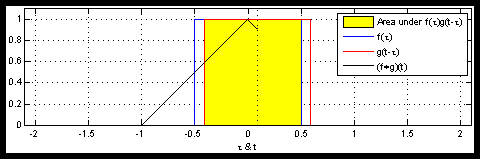
\includegraphics[scale=0.5]{diagrams/conv2}
	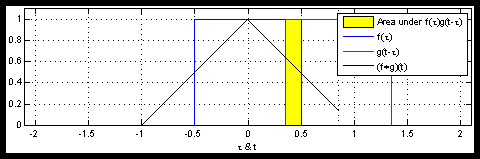
\includegraphics[scale=0.5]{diagrams/conv3}
\end{figure}

Formally this, equates to the following definition for convolution over continuous domains:
\begin{definition}
	The \textbf{convolution} $*$, of two functions $F$ and $G$ is defined as:
	\begin{equation}
		(F*G)(t) = \int_{-\infty}^\infty F(\tau) \;G(t - \tau) \; d\tau
	\end{equation}
\end{definition}
and in the case of discrete linear convolution, summation would replace integration.
In this equation, $t$ represents the translation of $G$ as well as the input for $(F*G)$
while $\tau$ is internal to the integral and varies over the real line.


\begin{figure}[ht]
	\caption[Gaussian Blurring]{512x512px ``Lena''(a) with a 1px (b) and 5px (c) Gaussian blur applied. 
	Gaussian blurring is accomplished by convolving an image with a Gaussian kernel and is commonly used
	in image processing to reduce noise prior to edge detection.
	\label{fig:LenaBlur}}
	\centering
	\begin{subfigure}[b]{0.3\textwidth}
                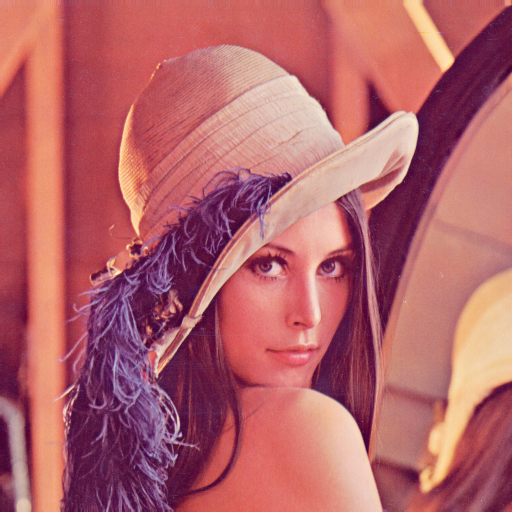
\includegraphics[scale=0.25]{diagrams/Lenna}
                \caption{Original Image}
       \end{subfigure}
       \begin{subfigure}[b]{0.3\textwidth}
                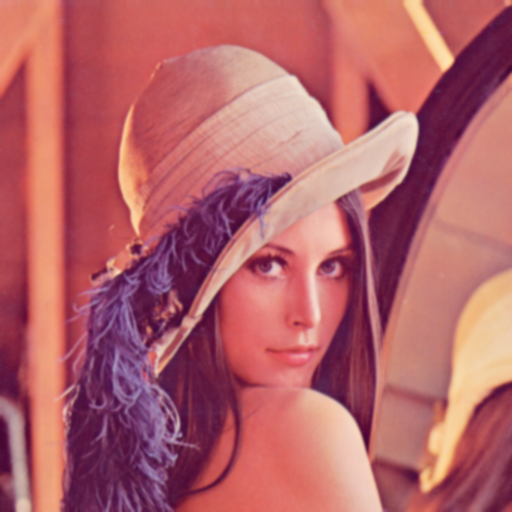
\includegraphics[scale=0.25]{diagrams/Lenna-blur1}
                \caption{1px Gaussian blur}
       \end{subfigure}
       \begin{subfigure}[b]{0.3\textwidth}
                
\includegraphics[scale=0.25]{diagrams/Lenna-blur5}
                \caption{5px Gaussian blur}
       \end{subfigure}
\end{figure}


Convolution has applications in many areas of mathematics and engineering.
One very common use in image processing is in blurring.
\emph{Gaussian blurring} is the result of a 2-dimensional convolution of an image with the Gaussian distribution function:
\begin{equation}
	\label{eqn:2dGaussian}
	G(x,y) = \frac{1}{2 \pi \sigma^2} \; \text{exp} \left( - \frac{x^2 + y^2}{2\sigma^2} \right)
\end{equation}
Blurring an image in this way reduces noise and greatly increases the efficacy of subsequent edge detection.
In statistics, a (simple) \emph{moving average} can be represented as a convolution by a rectangular pulse while more
generally, weighted moving averages can be made by convolving with other functions.





%%%%%%%%%%%%%%%%%%%%%%%%%%%%%%%%%%%%%%%%%
%
% CONVOLUTION OF PIECEWISE
%
%%%%%%%%%%%%%%%%%%%%%%%%%%%%%%%%%%%%%%%%%
\section{Convolution of Piecewise Functions}\label{sec:PWConvolution}


CAS such as Maple and Mathematica are quite adept at solving integrals.
Convolution of elementary functions generally poses no problem.
When convolving two piecewise continuous functions, many possible intervals arise and the conditionals that arise
can quickly overwhelm them unaided. \todo{cite, rewrite?}


We are interested in \emph{Symbolic Linear Convolution} (of piecewise continuous functions).
The typical approach is to first consider for convolution of ``one piece'' functions 
\cite{evans1994algorithms, west1993symbolic}.
By ``one-piece'' functions we mean functions which are restricted to a single interval and zero everywhere else.
We will consider two functions, $F$ and $G$ defined as:


\begin{equation}
	\label{eqn:fOnePiece}
	F(x)=f^{[a_f,b_f)}(x) = 
		\begin{cases}
			f(x) & a_f \leq x < b_f \\
			0 & \text{otherwise}
		\end{cases}
\end{equation}
\begin{equation}
	\label{eqn:gOnePiece}
	G(x)=g^{[a_g,b_g)}(x) = 
		\begin{cases}
			g(x) & a_g \leq x < b_g \\
			0 & \text{otherwise}
		\end{cases}
\end{equation}
for which we would like to compute the convolution $(F*G)$.
To reduce the total number of cases generated, it is generally also assumed that $b_f - a_f \leq b_g - a_g$.
Assuming that $F$ is non-zero over a shorter interval is not that strong an assumption as convolution is commutative;
if it is not the case we can rearrange $F*G$ to $G*F$.
To see this, simply apply the substitute $\tau' = t-\tau$ in equation (7.1):
\begin{align}
	\label{eqn:ConvCommutative}
	(F*G)(t) 
		&= \int_{-\infty}^\infty F(\tau) G(t-\tau) \;d \tau 
		\notag\\&= \int_{\infty}^{-\infty} F(t-\tau')G(\tau')\; (-1) d\tau' 
		\notag\\&= \int_{-\infty}^\infty G(\tau') F(t-\tau') \; d\tau'
		\notag\\&= (G*F)(t)
\end{align}


Thus we can assume that our static function is also the function with the shorter interval.
Since $F$ and $G$ are zero outside of their respective intervals, we do not need to integrate over the entire real line. 
$F$ is our static function, so $[a_f, b_f)$ would be sufficient.
For a tight boundary, we have the following:
\begin{align}
	\label{eqn:ConvNaiveOnePiece}
	(F*G)(t) 
	&= \int_{-\infty}^\infty F(\tau)\; G(t-\tau) \; d\tau \notag \\
	&= \int_{a_f}^{b_f} f(\tau) \; G(t-\tau) \; d\tau \notag \\
	&= 	\begin{cases}
			\int_{a_f}^{t-a_g} f(\tau) \; g(t-\tau) \; d\tau 	& (a_f+a_g) \leq t < (b_f+a_g) \\
			\int_{a_f}^{b_f} f(\tau) \; g(t-\tau) \; d\tau		& (b_f+a_g) \leq t < (a_f+b_g) \\
			\int_{t-b_g}^{b_f} f(\tau) \; g(t-\tau) \; d\tau	& (a_f+b_g) \leq t < (b_f+b_g) \\
			0										& \text{otherwise}
		\end{cases}
\end{align}


\begin{figure}[ht]
	\caption[Convolution of ``one-piece'' functions]{Convolution of length 1 and 2 rectangular pulses. 
	Given the functions $F=1^{[-1,1)}$ and $G=1^{[-2,2)}$, there are three non-zero regions in $(F*G)$.
	\label{fig:OnePiece}}
	\centering
	\begin{tikzpicture}
		\begin{axis}[
			x=1.5cm,
			y=1.5cm,
			xstep=1,
			ystep=1,
			xmin=-3.9,xmax=3.9,
			ymin=-0.4,ymax=2.4,
			axis x line=middle,
			axis y line=middle,
			axis line style=<->,
			xlabel={$x$},
			ylabel={$y$},
	        ]
		\addplot[no marks,black,very thick,<-] expression[domain=-3.9:-3,samples=100]{0};
		\addplot[no marks,black,very thick,-] expression[domain=-1:1,samples=100]{2};
		\addplot[no marks,black,very thick,-] expression[domain=-3:-1,samples=100]{x+3};
		\addplot[no marks,black,very thick,-] expression[domain=1:3,samples=100]{3-x};
		\addplot[no marks,black,very thick,->] expression[domain=3:3.9,samples=100]{0};
		\node(afag) at (axis cs:-3,2.25) {$a_f+a_g$};
		\node(bfag) at (axis cs:-1,2.25) {$b_f+a_g$};
		\node(afbg) at (axis cs:1,2.25) {$a_f+b_g$};
		\node(bfbg) at (axis cs:3,2.25) {$b_f+b_g$};
	        \end{axis}
		%\draw[thick,<->] (-4,0) -- (4,0);
		%\draw[thick,<->] (0,-.5) -- (0,1.5);
		
	\end{tikzpicture}
\end{figure}


These regions can be visualized as above in Figure~\ref{fig:OnePiece} where two rectangular pulses are convolved. 
If both functions had equal length non-zero intervals (i.e. $b_f-a_f = b_g-a_g$), then the central plateau would be empty
(as in Figure~\ref{fig:ConvolutionExample}).
Another formulation presented by C\^{i}rnu \cite{cirnu2012calculation} and Cavicchi \cite{cavicchi2002simplified} is to use:
\begin{equation}
	\label{eqn:ConvCirnu}
	(F*G)(t)=
	\begin{cases}
		\int_{\max(a_f, \; t-b_g)}^{\min(b_f, t-a_g)} f(\tau)\cdot g(t-\tau)\; d\tau & (a_f+a_g) \leq t < (b_f+b_g) \\
		0 & \text{otherwise}
	\end{cases}
\end{equation}
Although this may appear to reduce the number of cases, expanding the $\min$ and $\max$ will cause just as many 
cases to return.


To extend this to piecewise continuous function, 
we simply treat each piecewise function as the sum of ``one-piece'' functions.
Given functions, $F= \sum_i f_i^{P_i}$ and $G= \sum_j g_j^{Q_j}$ 
where $\{P_i\}$, $\{Q_j\}$ are each sets of disjoint intervals, and $f_i^{P_i}$, $g_j^{Q_j}$ are all ``one-piece'' functions.
The convolution of $F*G$ is the sum of pairwise convolution:

\begin{align}
	\label{eqn:ConvPiecewise}
	\left(\left(\sum_i f_i^{P_i}\right) * \left(\sum_j g_j^{Q_j}\right)\right) (t)
	&= \int_{-\infty}^\infty \left(\sum_i f_i^{P_i}\right)(\tau)\cdot \left(\sum_j g_j^{Q_j}\right)(t-\tau) \;d\tau
	\notag\\&= \sum_i \sum_j \int_{-\infty}^\infty f_i^{P_i}(\tau) \cdot g_j^{Q_j}(t-\tau) \;d\tau 
	\notag\\&= \sum_i \sum_j \left(f_i^{P_i} * g_j^{P_j}\right)
\end{align}


This is the typical approach to convolution of piece-wise functions originally presented by West and McClellan 
\cite{west1993symbolic}.
When the boundaries between regions is symbolic, then we may not be able to determine which interval is longer.
Another approach involving hybrid functions will be presented in Section~\ref{sec:HFConvolution}. 
Concerns with intervals where one boundary point is at infinity have also been raised \cite{evans1994algorithms}.
Techniques to handle this will be investigated in Section~\ref{sec:ConvInfty}.








%%%%%%%%%%%%%%%%%%%%%%%%%%%%%%%%%%%%%%%%%
%
% HYBRID CONVOLUTION
%
%%%%%%%%%%%%%%%%%%%%%%%%%%%%%%%%%%%%%%%%%
\section{Hybrid Function Convolution}
\label{sec:HFConvolution}

Our exposition for hybrid set convolution will appear very similar to that from the previous section.
Again we will be interested in the convolution of ``one-piece'' functions which we will use to build up piece-wise
continuous functions.
So assume hybrid functions $F=f^{[a_f, b_f)}$ and $G=g^{[a_g,b_g)}$.
We do \emph{not} enforce that $b_f - a_f \leq b_g - a_g$ as we did in Section~\ref{sec:PWConvolution}.
Instead both cases will be handled by our generalized partition structure.


\begin{align}
	(f^{[a_f,b_f)} \;*\; g^{[a_g,b_g)}) (t) = 
		\R[+] &\left( \; \left( 
			\int_{[\![a_f,\;t-a_g)\!)} f(\tau) \; g(t-\tau) \; d\tau \right)^{[\![a_f+a_g,\; b_f+a_g)\!)} 
				\right. \notag \\ &\oplus \left( 
			\int_{[\![a_f,\;b_f)\!)} f(\tau) \; g(t-\tau) \; d\tau \right)^{[\![b_f+a_g,\; a_f+b_g)\!)} 
				\notag \\ &\oplus \left. \left( 
			\int_{[\![t-b_g,\;b_f)\!)} f(\tau) \; g(t-\tau) \; d\tau \right)^{[\![a_f+b_g,\; b_f+b_g)\!)} 
				\; \right)(t)
\end{align}

The first thing one should note is the similarity between this expression and (\ref{eqn:ConvNaiveOnePiece}).
When $b_f - a_f \leq b_g - a_g$ then the three oriented intervals will be disjoint and the two equations are identical.
Otherwise, if $b_f - a_f > b_g - a_g$, then the interval $[\![b_f +a_g, \; a_f + b_g)\!)$ will have a negative orientation.
The intervals $[\![a_f+a_g, \; b_f+a_g)\!)$, $[\![b_f+a_g, \; a_f+b_g)\!)$ and $[\![a_f+b_g, \; b_f+b_g)\!)$ still forms
a reducible (i.e. everywhere multiplicity one) generalized partition over $[a_f+a_g, \; b_f+b_g)$.
Outside this region the function is zero as expected. 


Suppose we are in this second case and we wish to evaluate the convolution at a point $t$ which is in all three intervals.
This occurs when $(a_f+b_g) \leq t < (b_f+a_g)$ and we have:
\begin{align*}
	[\![a_f+a_g, \; b_f+a_g)\!)(t) &= 1 \\
	[\![b_f+a_g, \; a_f+b_g)\!)(t) &= -1 \\
	[\![a_f+b_g,\; b_f+b_g)\!)(t) &= 1
\end{align*}
Simplifying the $+$-reduction we then get:
\begin{align}
	(f^{[a_f,b_f)} \;*\; g^{[a_g,b_g)}) (t) = 
		& \; \left( 
			\int_{[\![a_f,\;t-a_g)\!)} f(\tau) \; g(t-\tau) \; d\tau \right) 
				\notag \\ &- \left( 
			\int_{[\![a_f,\;b_f)\!)} f(\tau) \; g(t-\tau) \; d\tau \right)
				\notag \\ &+ \left( 
			\int_{[\![t-b_g,\;b_f)\!)} f(\tau) \; g(t-\tau) \; d\tau \right) 
\end{align}
All three of these integrals have the same integrand so we can use bi-linearity to move the sum to be over the domains
of integration.
These domains then cancel nicely to leave us with:
\begin{align}
	\label{eqn:HybridConvMidFinal}
	(f^{[a_f,b_f)} \;*\; g^{[a_g,b_g)}) (t) = &
		\int_{[\![a_f,\;t-a_g)\!) \;\ominus\; [\![a_f,\;b_f)\!) \;\oplus\; [\![t-b_g,\;b_f)\!)} f(\tau) \; g(t-\tau) \; d\tau \notag\\
		= & \int_{[\![t-b_g,\;t-a_g)\!)} f(\tau) \; g(t-\tau) \; d\tau
\end{align}
Let us now look at a concrete example with some actual numbers.


%%%%%%%%%%%%%%%%%%%%%%%%%%%%%%%%%%%%%%%%%
% HYBRID EXAMPLE
%%%%%%%%%%%%%%%%%%%%%%%%%%%%%%%%%%%%%%%%%
\subsection{Example: \emph{Hybrid Convolution}}


In Figure~\ref{fig:OnePiece} we saw the convolution of $1^{[-1,1)}$ with $1^{[-2,2)}$.
We know that convolution is commutative so computing $1^{[-2,2)} * 1^{[-1,1)}$ we already know what to expect.
We will label these as $1_f$ and $1_g$ to differentiate and to prevent confusion by reminding us that the object we are 
dealing with is $x \mapsto 1$ rather than the number 1 itself.
\begin{align}
	\label{HCExample}
	(1_f^{[-2,2)} \;*\; 1_g^{[-1,1)}) (t) = 
		\R[+] &\left( \; \left( 
			\int_{[\![-2,\;t-1)\!)} f(\tau) \; g(t-\tau) \; d\tau \right)^{[\![-3,\; 1)\!)} 
				\right. \notag \\ &\oplus \left( 
			\int_{[\![-2,\;1)\!)} f(\tau) \; g(t-\tau) \; d\tau \right)^{[\![1,\; -1)\!)} 
				\notag \\ &\oplus \left. \left( 
			\int_{[\![t-1,\;2)\!)} f(\tau) \; g(t-\tau) \; d\tau \right)^{[\![-1,\; 3)\!)} 
				\; \right)(t)
\end{align}


Already this is promising as we can see the set of end-points: $\{-3, -1, 1, 3\}$ agrees with our previous example.
Let us consider three points $t_1 \in [-3, -1)$, $t_2 \in [-1, 1)$ and $t_3 \in [1,3)$.
We omit the derivations but encourage the reader to convince themselves that each is correct.
\begin{equation*}
	(1_f^{[-2,2)} \;*\; 1_g^{[-1,1)}) (t_1) 
		\;=\; \int_{[\![-2,\;t_1-(-1))\!)} 1_f(\tau) \; 1_g(t_1-\tau) \; d\tau
		\;=\; t_1 + 3
\end{equation*}
First we should note that at no point in the integral do we attempt to evaluate $1_f$ or $1_g$ outside of their original 
domains $[-2,2]$ and $[-1,1]$ respectively. 
Thus it is safe to replace $1_f(\tau)\cdot 1_g(t-\tau)$ with 1  inside the integral.
From here, the integral is trivially evaluated and is as expected.

For $t_3$, only the third term has non-zero multiplicity and by an identical argument as for $t_1$ we have:
\begin{equation*}
	(1_f^{[-2,2)} \;*\; 1_g^{[-1,1)}) (t_3) 
		\;=\; \int_{[\![t-1,2)\!)} 1_f(\tau) \; 1_g(t_3-\tau) \; d\tau
		\;=\; 3 - t_3
\end{equation*}
Finally, $t_2$ deviates from this pattern slightly as $t_2$ is in \emph{all three} oriented intervals.
By the same derivation as we used in the previous section we can use equation~(\ref{eqn:HybridConvMidFinal}):
\begin{equation*}
	\label{eqn:HCExampleT2}
	(1_f^{[a_f,b_f)} \;*\; 1_g^{[a_g,b_g)}) (t_2) 
		\;=\; \int_{[\![t_2-1,\;t_2-(-1))\!)} f(\tau) \; g(t-\tau) \; d\tau
		\;=\; 2
\end{equation*}
For any other point $t$ which is not in $[-3, 3)$, then all three oriented intervals will have multiplicity zero.
Simplifying the $+$-reduction we have, $\R[+](\emptyset) = e_+ = 0$ and so (\ref{HCExample}) evaluates correctly 
everywhere.




%%%%%%%%%%%%%%%%%%%%%%%%%%%%%%%%%%%%%%%%%
%
% INFINITE INTERVALS
%
%%%%%%%%%%%%%%%%%%%%%%%%%%%%%%%%%%%%%%%%%
\section{Infinite Intervals}\label{sec:ConvInfty}


The method for computing convolution in the previous section works for finite end points over the real line but if we
move to infinite end points on the extended real line, things break down.




%%%%%%%%%%%%%%%%%%%%%%%%%%%%%%%%%%%%%%%%%
%
% EXAMPLE
%
%%%%%%%%%%%%%%%%%%%%%%%%%%%%%%%%%%%%%%%%%
\section{Example}

\newpage
\include{conclusion}


%% This adds a line for the Bibliography in the Table of Contents.
\addcontentsline{toc}{chapter}{Bibliography}
%% ***   Set the bibliography style.   ***
\bibliographystyle{plain} % (change according to your preference)
%%% ***   Set the bibliography file.   ***
\bibliography{westernthesis}{}
%% ***   NOTE   ***
%% If you don't use bibliography files, comment out the previous line
%% and use \begin{thebibliography}...\end{thebibliography}.  (In that
%% case, you should probably put the bibliography in a separate file
%% and \include or \input it here).

%Appendices.
\begin{appendices}
\def\ind[#1]{\mathbb{I}_{#1}}
\def\extendedreal{\bar{\mathbb{R}}}
\def\hsetover[#1]{\mathbb{Z}^{#1}}

\chapter{Integration III} \label{integration}
\doublespacing

``Chapter goals''

Section 4.1 will cover a conventional treatment of the Lebesgue integral, for those already familiar with the construction, this may be skipped. 

%%%%%%%%%%%%%%%%%%%%%%%%%%%%%%%%%%%%%%%%%
%
% LEBESGUE INTEGRATION
%
%%%%%%%%%%%%%%%%%%%%%%%%%%%%%%%%%%%%%%%%%

\section{Sigma Algebras}

Before we can talk about the Lebesgue integral we must first set the stage, so to speak.



\begin{definition}
Let $X$ be a non-empty set. A \textbf{$\sigma$-algebra on the set $X$}, $\Sigma$,  is a family of subsets of $X$ such that:
\begin{enumerate}
\item $\Sigma$ is non-empty
\item \emph{Closed under complement.} If $E \in \Sigma$, then $X \setminus E \in \Sigma$.
\item \emph{Closed under countable union.} If $E_1, E_2, ... \in \Sigma$ then $(E_1 \cup E_2 \cup ... ) \in \Sigma$.
\end{enumerate}
The pair $(X, \Sigma)$ is called a \textbf{measurable space} and elements of $\Sigma$ are called the \textbf{measurable sets} (of $X$).
\end{definition}

It can easily be shown through the use of De Morgan's laws that a $\sigma$-algebra is also closed under countable intersection as well.
\begin{example}
$\{ \emptyset, X \}$ is a $\sigma$-algebra on $X$. In fact, $X$ and $\emptyset$ are members of \emph{every} $\sigma$-algebra on $X$.
\end{example}

\begin{example}
$2^X$ is a $\sigma$-algebra on $X$.
\end{example}

However, we would also like to be able to construct more interesting $\sigma$-algebras.

\begin{definition}
Given an arbitrary family of subsets $F \subseteq 2^X$, there is a unique smallest $\sigma$-algebra containing $F$ which is called the \textbf{$\mathbf{\sigma}$-algebra generated by $F$} and we will denote as $\sigma(F)$.
\end{definition}

Can be constructed by taking the intersection of all $\sigma$-algebras containing $F$.

Of particular interest to us is the $\sigma$-algebra generated by a topology, $\mathcal{T}(X)$. 

Borel $\sigma$-algebra: $\mathcal{B}(X) = \sigma(\mathcal{T}(X))$



\chapter{Convolution with Infinite End-Points}
\label{chp:16cases}


\begin{table}[h]
\caption[Possible combinations of finite and infinite end-points]{
	All possible cases of finite and infinite end-points. Finite end-points are denoted with $F$. Infinite left end-points are denoted 	
	$-\infty$ and infinite right end-points are denoted $\infty$.
	\label{fig:16cases}}
\centering
\begin{tabular}{| l || c | c | c | c || r || l ||  c | c | c | c |}
	\hline
		& $a_f$		& $b_f$		& $a_g$		& $b_g$	&$\;\;\;\;$&	& $a_f$		& $b_f$		& $a_g$		& $b_g$	\\
	\hline 
\textit{Case 0:}& $F$	& $F$		& $F$		& $F$	&&	Case 8:	& $-\infty$	& $F$		& $F$		& $F$	\\
Case 1:	& $F$		& $F$		& $F$		& $\infty$&&	Case 9:	& $-\infty$	& $F$		& $F$		& $\infty$ \\
Case 2:	& $F$		& $F$		& $-\infty$	& $F$	&&	Case 10:	& $-\infty$	& $F$		& $-\infty$	& $F$	\\
Case 3:	& $F$		& $F$		& $-\infty$	& $\infty$&&	Case 11:	& $-\infty$	& $F$		& $-\infty$	& $\infty$ \\
Case 4:	& $F$		& $\infty$	& $F$		& $F$	&&	Case 12:	& $-\infty$	& $\infty$	& $F$		& $F$	\\
Case 5:	& $F$		& $\infty$ 	& $F$		& $\infty$&&	Case 13:	& $-\infty$	& $\infty$ 	& $F$		& $\infty$ \\
Case 6:	& $F$		& $\infty$ 	& $-\infty$	& $F$	&&	Case 14:	& $-\infty$	& $\infty$ 	& $-\infty$	& $F$	\\
Case 7:	& $F$		& $\infty$ 	& $-\infty$	& $\infty$&&	Case 15:	& $-\infty$	& $\infty$ 	& $-\infty$	& $\infty$ \\
	\hline
\end{tabular}
\end{table}


When convolving one-piece functions with infinite end-points, there are 4 end-points which can each be either finite or infinite.
As such there are $2^4$ possible combinations of end-point types shown in the table above.
Throughout all calculations in this section, the integrands will not change, only the domains.
So we define the function $\C$ as a sort of restricted convolution:
\begin{equation}
	\C[ [\![x,y)\!) ](t) = \int_{[\![x,y)\!)} f(\tau) g(t-\tau) \; d\tau
\end{equation}
Which can be used to condense equation~(\ref{eqn:defHConvolution}), the definition for hybrid convolution, into:
\begin{align*}
	\label{eqn:defHConvolution2}
	(f^{[a_f,b_f)} \;*\; g^{[a_g,b_g)})
		= \R[+] &\left( \; 
			{\C[ [\![a_f,\;t-a_g)\!) ]}^{[\![a_f+a_g,\; b_f+a_g)\!)} \oplus
			{\C[ [\![a_f,\;b_f)\!) ]}^{[\![b_f+a_g,\; a_f+b_g)\!)} \oplus
			{\C[ [\![t-b_g,\;b_f)\!) ]}^{[\![a_f+b_g,\; b_f+b_g)\!)} 
		\; \right)
\end{align*}


%%%%%%%%%%%%%%%%%%%%%%%%%%%%%%%%%%%%%%%%%
\textbf{Case 0} has all finite points and was already shown to be correct in Section~\ref{sec:HFConvolution} but is listed
for completeness.
The exposition will not be repeated here.


%%%%%%%%%%%%%%%%%%%%%%%%%%%%%%%%%%%%%%%%%
\textbf{Case 1} has one infinite point, $b_g = \infty$ and results in an empty interval for the third term.
Since it is impossible for $t$ to be in $[\![\infty, \infty )\!)$, we can safely remove this term altogether.
\begin{align*}
	(f^{[a_f,b_f)} \;*\; g^{[a_g,\infty)})
	= \R[+] &\left( \;
			{\C[ [\![a_f,\;t-a_g)\!) ]}^{[\![a_f+a_g,\; b_f+a_g)\!)} \oplus
			{\C[ [\![a_f,\;b_f)\!) ]}^{[\![b_f+a_g,\; \infty)\!)} \oplus
			{\C[ [\![-\infty,\;b_f)\!) ]}^{[\![\infty,\; \infty)\!)} 
		\; \right)\\
	= \R[+] &\left( \;
			{\C[ [\![a_f,\;t-a_g)\!) ]}^{[\![a_f+a_g,\; b_f+a_g)\!)} \oplus
			{\C[ [\![a_f,\;b_f)\!) ]}^{[\![b_f+a_g,\; \infty)\!)}
		\; \right)
\end{align*}


Throughout this section we will use sets of diagrams like the one below to verify that our expressions are sensible.
The region where the intervals, $[a_f, b_f)$ and $[t-b_g, t-a_g)$ overlap, (shaded in gray) is where the convolution 
will be non-zero.
The bounds of this intersection may depend on $t$; each case that results in a non-empty intersection will be
shown separately.
To verify an expression, each diagram should correspond to a term in the convolution and the bounds of the shaded 
region should correspond to the domain on that term's integral.
\begin{figure}[h]
	\centering
	\begin{subfigure}[h]{0.4\textwidth}
		\caption{$t \in [\![a_f+a_g, \; b_f+a_g)\!)$} 
		\centering
		\begin{tikzpicture}
			\draw[fill, color=black!20] (0,0) rectangle (1,1);
			\draw[->] 
				(1,0) node[below](ag){$t-a_g$} 
				-- (1,1) 
				-- (-2,1);
			\draw 
				(0,0) node[below](af){$a_f$} 
				-- (0,1.2) 
				-- (2,1.2) 
				-- (2,0) node[below](bf){$b_f$};
		\end{tikzpicture}
	\end{subfigure}
	\begin{subfigure}[h]{0.4\textwidth}
		\caption{$t \in [\![b_f+a_g, \infty)\!)$} 
		\centering
		\begin{tikzpicture}
			\draw[fill, color=black!20] (0,0) rectangle (2,1);
			\draw[->] 
				(3,0) node[below](ag){$t-a_g$} 
				-- (3,1) 
				-- (-1,1);
			\draw 
				(0,0) node[below](af){$a_f$} 
				-- (0,1.2) 
				-- (2,1.2) 
				-- (2,0) node[below](bf){$b_f$};
		\end{tikzpicture}
	\end{subfigure}
\end{figure}


%%%%%%%%%%%%%%%%%%%%%%%%%%%%%%%%%%%%%%%%%
\textbf{Case 2} also has only one infinite point, $a_g=-\infty$ and also yields an empty interval:
\begin{align*}
	(f^{[a_f,b_f)} \;*\; g^{[-\infty,b_g)}) 
	= \R[+] &\left( \; 
			{\C[ [\![a_f,\;\infty)\!) ]}^{[\![-\infty,\; -\infty)\!)} \oplus
			{\C[ [\![a_f,\;b_f)\!) ]}^{[\![-\infty,\; a_f+b_g)\!)} \oplus
			{\C[ [\![t-b_g,\;b_f)\!) ]}^{[\![a_f+b_g,\; b_f+b_g)\!)} 
		\; \right)\\
	= \R[+] &\left( \; 
			{\C[ [\![a_f,\;b_f)\!) ]}^{[\![-\infty,\; a_f+b_g)\!)} \oplus
			{\C[ [\![t-b_g,\;b_f)\!) ]}^{[\![a_f+b_g,\; b_f+b_g)\!)} 
		\; \right)
\end{align*} 
\vspace{-1cm}
\begin{figure}[h]
	\centering
	\begin{subfigure}{0.4\textwidth}
		\caption{$t \in [\![-\infty, \; a_f+b_g)\!)$} 
		\centering
		\begin{tikzpicture}
			\draw[fill, color=black!20] (0,0) rectangle (2,1);
			\draw[->] 
				(-1,0) node[below](ag){$t-b_g$} 
				-- (-1,1) 
				-- (3,1);
			\draw 
				(0,0) node[below](af){$a_f$} 
				-- (0,1.2) 
				-- (2,1.2) 
				-- (2,0) node[below](bf){$b_f$};
		\end{tikzpicture}
	\end{subfigure}
	\begin{subfigure}{0.4\textwidth}
		\caption{$t \in [\![a_f+b_g, b_f+b_g)\!)$} 
		\centering
		\begin{tikzpicture}
			\draw[fill, color=black!20] (1,0) rectangle (2,1);
			\draw[->] 
				(1,0) node[below](ag){$t-b_g$} 
				-- (1,1) 
				-- (4,1);
			\draw 
				(0,0) node[below](af){$a_f$} 
				-- (0,1.2) 
				-- (2,1.2) 
				-- (2,0) node[below](bf){$b_f$};
		\end{tikzpicture}
	\end{subfigure}
\end{figure}

\pagebreak
%%%%%%%%%%%%%%%%%%%%%%%%%%%%%%%%%%%%%%%%%
\textbf{Case 3} is a combination of both case 1 and 2, resulting in only a single term for the entire real line since
both the first and third terms are over empty intervals.
\begin{align*}
	(f^{[a_f,b_f)} \;*\; g^{[-\infty, \infty)})
	= \R[+] &\left( \; 
			{\C[ [\![a_f,\;\infty)\!) ]}^{[\![-\infty,\; -\infty)\!)} \oplus
			{\C[ [\![a_f,\;b_f)\!) ]}^{[\![-\infty,\; \infty)\!)} \oplus
			{\C[ [\![-\infty,\;b_f)\!) ]}^{[\![\infty,\; \infty)\!)} 
		\; \right) \\
	= \R[+] &\left( \; 
			{\C[ [\![a_f,\;b_f)\!) ]}^{[\![-\infty,\; \infty)\!)} 
		\;\right) 
		=\int_{[\![a_f,\;b_f)\!)} f(\tau) \; g(t-\tau) \; d\tau
\end{align*}
\vspace{-1.5cm}
\begin{figure}[h]
	\centering
	\begin{subfigure}[h]{0.4\textwidth}
		\caption{$t \in [\![-\infty, \; \infty)\!)$} 
		\centering
		\begin{tikzpicture}
			\draw[fill, color=black!20] (0,0) rectangle (2,1);
			\draw[<->] 
				(-1,1)
				-- (3,1);
			\draw 
				(0,0) node[below](af){$a_f$} 
				-- (0,1.2) 
				-- (2,1.2) 
				-- (2,0) node[below](bf){$b_f$};
		\end{tikzpicture}
	\end{subfigure}
\end{figure}


%%%%%%%%%%%%%%%%%%%%%%%%%%%%%%%%%%%%%%%%%
\textbf{Case 4} (i.e. $b_f = \infty$) is a bit more involved:
\begin{align*}
	(f^{[a_f,\infty)} \;*\; g^{[-\infty,b_g)}) 
	= \R[+] &\left( \; 
			{\C[ [\![a_f,\;t-a_g)\!) ]}^{[\![a_f+a_g,\; \infty)\!)} \oplus
			{\C[ [\![a_f,\;\infty)\!) ]}^{[\![\infty,\; a_f+b_g)\!)} \oplus
			{\C[ [\![t-b_g,\;\infty)\!) ]}^{[\![a_f+b_g,\; \infty)\!)} 
		\; \right) \\
	= \R[+] &\left( \; 
			{\C[ [\![a_f,\;t-a_g)\!) ]}^{[\![a_f+a_g,\; a_f+b_g)\!) \oplus[\![a_f+b_g,\; \infty)\!)} \ominus
			{\C[ [\![a_f,\;\infty)\!) ]}^{[\![a_f+b_g,\; \infty)\!)} \oplus
			{\C[ [\![t-b_g,\;\infty)\!) ]}^{[\![a_f+b_g,\; \infty)\!)} 
		\; \right) \\
	= \R[+] &\left( \; 
			{\C[ [\![a_f,\;t-a_g)\!) ]}^{[\![a_f+a_g,\; a_f+b_g)\!)} \oplus
			{\C[ [\![a_f,\;t-a_g)\!) \ominus [\![a_f,\;\infty)\!) \oplus [\![t-b_g,\;\infty)\!)  ]}^{[\![a_f+b_g,\; \infty)\!)} 
		\; \right) \\
	= \R[+] &\left( \; 
			{\C[ [\![a_f,\;t-a_g)\!) ]}^{[\![a_f+a_g,\; a_f+b_g)\!)} \oplus
			{\C[ [\![t-b_g,\;t-a_g)\!)  ]}^{[\![a_f+b_g,\; \infty)\!)} 
		\; \right)
\end{align*}
\vspace{-1.5cm}
\begin{figure}[h]
	\centering
	\begin{subfigure}[h]{0.4\textwidth}
		\caption{$t \in [\![a_f+a_g, a_f+b_g)\!)$} 
		\centering
		\begin{tikzpicture}
			\draw[fill, color=black!20] (1,0) rectangle (2,1);
			\draw 
				(0,0) node[below](ag){$t-b_g$} 
				-- (0,1) 
				-- (2,1)
				-- (2,0) node[below](af){$t-a_g$};
			\draw[->] 
				(1,0) node[below](af){$a_f$} 
				-- (1,1.2) 
				-- (4,1.2);
		\end{tikzpicture}
	\end{subfigure}
	\begin{subfigure}[h]{0.4\textwidth}
		\caption{$t \in [\![a_f+b_g, \infty)\!)$} 
		\centering
		\begin{tikzpicture}
			\draw[fill, color=black!20] (0,0) rectangle (2,1);
			\draw
				(0,0) node[below](bg){$t-b_g$} 
				-- (0,1) 
				-- (2,1)
				-- (2,0) node[below](ag){$t-a_g$};
			\draw[->]
				(-1,0) node[below](af){$a_f$} 
				-- (-1,1.2) 
				-- (3,1.2);
		\end{tikzpicture}
	\end{subfigure}
\end{figure}

%%%%%%%%%%%%%%%%%%%%%%%%%%%%%%%%%%%%%%%%%
\textbf{Case 5} $b_f =\infty$, $b_g = \infty$
\begin{align*}
	(f^{[a_f,\infty)} \;*\; g^{[a_g,\infty)})
		= \R[+] &\left( \; 
			{\C[ [\![a_f,\;t-a_g)\!) ]}^{[\![a_f+a_g,\; \infty)\!)} \oplus
			{\C[ [\![a_f,\;\infty)\!) ]}^{[\![\infty,\; \infty)\!)} \oplus
			{\C[ [\![-\infty,\; \infty)\!) ]}^{[\![\infty,\; \infty)\!)} 
		\; \right)\\
		=\R[+] &\left( \; 
			{\C[ [\![a_f,\;t-a_g)\!) ]}^{[\![a_f+a_g,\; \infty)\!)}
		\; \right)
\end{align*}
\vspace{-1.5cm}
\begin{figure}[h]
	\centering
	\begin{subfigure}[h]{0.4\textwidth}
		\caption{$t \in [\![a_f+a_g, \; \infty)\!)$} 
		\centering
		\begin{tikzpicture}
			\draw[fill, color=black!20] (0,0) rectangle (2,1);
			\draw[->] 
				(2,0) node[below](ag){$t-a_g$}
				-- (2,1)
				-- (-1,1);
			\draw[->]
				(0,0) node[below](af){$a_f$} 
				-- (0,1.2) 
				-- (3,1.2);
		\end{tikzpicture}
	\end{subfigure}
\end{figure}

%%%%%%%%%%%%%%%%%%%%%%%%%%%%%%%%%%%%%%%%%
\textbf{Case 6:} $b_f=\infty$, $a_g =-\infty$
\begin{align*}
	(f^{[a_f,\infty)} \;*\; g^{[-\infty,b_g)})
	= \R[+] &\left( \; 
			{\C[ [\![a_f,\;\infty)\!) ]}^{[\![-\infty,\; \bot)\!)} \oplus
			{\C[ [\![a_f,\;\infty)\!) ]}^{[\![\bot,\; a_f+b_g)\!)} \oplus
			{\C[ [\![t-b_g,\;\infty)\!) ]}^{[\![a_f+b_g,\;\infty)\!)} 
		\; \right) \\
	= \R[+] &\left( \; 
			{\C[ [\![a_f,\;\infty)\!) ]}^{[\![-\infty,\; a_f+b_g)\!)} \oplus
			{\C[ [\![t-b_g,\;\infty)\!) ]}^{[\![a_f+b_g,\;\infty)\!)} 
		\; \right)
\end{align*}
\vspace{-1.5cm}
\begin{figure}[h]
	\centering
	\begin{subfigure}[h]{0.4\textwidth}
		\caption{$t \in [\![-\infty, a_f+b_g)\!)$} 
		\centering
		\begin{tikzpicture}
			\draw[fill, color=black!20] (1,0) rectangle (3,1);
			\shade[left color=black!20, right color=white] (3,0) rectangle (4,1);
			\draw[->]
				(0,0) node[below](bg){$t-b_g$} 
				-- (0,1) 
				-- (4,1);
			\draw[->] 
				(1,0) node[below](af){$a_f$} 
				-- (1,1.2) 
				-- (4,1.2);
		\end{tikzpicture}
	\end{subfigure}
	\begin{subfigure}[h]{0.4\textwidth}
		\caption{$t \in [\![a_f+b_g, \infty)\!)$} 
		\centering
		\begin{tikzpicture}
			\draw[fill, color=black!20] (1,0) rectangle (3,1);
			\shade[left color=black!20, right color=white] (3,0) rectangle (4,1);
			\draw[->]
				(1,0) node[below](bg){$t-b_g$} 
				-- (1,1) 
				-- (4,1);
			\draw[->] 
				(0,0) node[below](af){$a_f$} 
				-- (0,1.2) 
				-- (4,1.2);
		\end{tikzpicture}
	\end{subfigure}
\end{figure}

%%%%%%%%%%%%%%%%%%%%%%%%%%%%%%%%%%%%%%%%%
\textbf{Case 7:} $b_f=\infty$, $a_g =-\infty$, $b_g=\infty$
\begin{align*}
	(f^{[a_f,\infty)} \;*\; g^{[-\infty,\infty)})
	= \R[+] &\left( \; 
			{\C[ [\![a_f,\;\infty)\!) ]}^{[\![-\infty,\; \bot)\!)} \oplus
			{\C[ [\![a_f,\;\infty)\!) ]}^{[\![\bot,\; \infty)\!)} \oplus
			{\C[ [\![-\infty,\;\infty)\!) ]}^{[\![\infty,\; \infty)\!)} 
		\; \right) \\
	= \R[+] &\left( \; 
			{\C[ [\![a_f,\;\infty)\!) ]}^{[\![-\infty,\; \infty)\!)}
		\; \right)
\end{align*}
\vspace{-1.5cm}
\begin{figure}[h]
	\centering
	\begin{subfigure}[h]{0.4\textwidth}
		\caption{$t \in [\![-\infty, \; \infty)\!)$} 
		\centering
		\begin{tikzpicture}
			\draw[fill, color=black!20] (0,0) rectangle (2,1);
			\shade[left color=black!20, right color=white] (2,0) rectangle (3,1);
			\draw[<->] 
				(-1,1)
				-- (3,1);
			\draw[->]
				(0,0) node[below](af){$a_f$} 
				-- (0,1.2) 
				-- (3,1.2);
		\end{tikzpicture}
	\end{subfigure}
\end{figure}


%%%%%%%%%%%%%%%%%%%%%%%%%%%%%%%%%%%%%%%%%
\textbf{Case 8:} $a_f=-\infty$
\begin{align*}
	(f^{[-\infty,b_f)} \;*\; g^{[a_g,b_g)})
	= \R[+] &\left( \; 
			{\C[ [\![-\infty,\;t-a_g)\!) ]}^{[\![-\infty,\; b_f+a_g)\!)} \oplus
			{\C[ [\![-\infty,\;b_f)\!) ]}^{[\![b_f+a_g,\; -\infty)\!)} \oplus
			{\C[ [\![t-b_g,\;b_f)\!) ]}^{[\![-\infty,\; b_f+b_g)\!)} 
		\; \right) \\	
	= \R[+] &\left( \; 
			{\C[ [\![-\infty,\;t-a_g)\!) ]}^{[\![-\infty,\; b_f+a_g)\!)} \ominus
			{\C[ [\![-\infty,\;b_f)\!) ]}^{[\![-\infty, \; b_f+a_g)\!)} \oplus
			{\C[ [\![t-b_g,\;b_f)\!) ]}^{[\![-\infty,\; b_f+a_g)\!)\oplus[\![b_f+a_g, b_f+b_g)\!)} 
		\; \right) \\
	= \R[+] &\left( \; 
			{\C[ [\![-\infty,\;t-a_g)\!)
				\ominus[\![-\infty,\;b_f)\!)
				\oplus[\![t-b_g,\;b_f)\!) ]}^{[\![-\infty,\; b_f+a_g)\!)} \oplus
			{\C[ [\![t-b_g,\;b_f)\!) ]}^{[\![b_f+a_g, b_f+b_g)\!)} 
		\; \right) \\
	= \R[+] &\left( \; 
			{\C[ [\![t-b_g,\;t-a_g)\!) ]}^{[\![-\infty,\; b_f+a_g)\!)} \oplus
			{\C[ [\![t-b_g,\;b_f)\!) ]}^{[\![b_f+a_g, b_f+b_g)\!)} 
		\; \right)
\end{align*}
\vspace{-1.5cm}
\begin{figure}[h]
	\centering
	\begin{subfigure}[h]{0.4\textwidth}
		\caption{$t \in [\![-\infty, b_f+a_g)\!)$} 
		\centering
		\begin{tikzpicture}
			\draw[fill, color=black!20] (0,0) rectangle (2,1);
			\draw[->] 
				(3,0) node[below](bf){$b_f$} 
				-- (3,1.2) 
				-- (-1,1.2);
			\draw 
				(0,0) node[below](bg){$t-b_g$} 
				-- (0,1) 
				-- (2,1) 
				-- (2,0) node[below](ag){$t-a_g$};
		\end{tikzpicture}
	\end{subfigure}
	\begin{subfigure}[h]{0.4\textwidth}
		\caption{$t \in [\![b_f+a_g, b_f+b_g)\!)$} 
		\centering
		\begin{tikzpicture}
			\draw[fill, color=black!20] (0,0) rectangle (1,1);
			\draw 
				(0,0) node[below](bg){$t-b_g$} 
				-- (0,1) 
				-- (2,1) 
				-- (2,0) node[below](ag){$t-a_g$};
			\draw[->] 
				(1,0) node[below](bf){$b_f$} 
				-- (1,1.2) 
				-- (-2,1.2);
		\end{tikzpicture}
	\end{subfigure}
\end{figure}


%%%%%%%%%%%%%%%%%%%%%%%%%%%%%%%%%%%%%%%%%
\textbf{Case 9:} $a_f=-\infty$, $b_g=\infty$
\begin{align*}
	(f^{[-\infty,b_f)} \;*\; g^{[a_g,\infty)})
	= \R[+] &\left( \; 
			{\C[ [\![-\infty,\;t-a_g)\!) ]}^{[\![-\infty,\; b_f+a_g)\!)} \oplus
			{\C[ [\![-\infty,\;b_f)\!) ]}^{[\![b_f+a_g,\; \bot)\!)} \oplus
			{\C[ [\![-\infty,\;b_f)\!) ]}^{[\![\bot,\;\infty)\!)} 
		\; \right) \\
	= \R[+] &\left( \; 
			{\C[ [\![-\infty,\;t-a_g)\!) ]}^{[\![-\infty,\; b_f+a_g)\!)} \oplus
			{\C[ [\![-\infty,\;b_f)\!) ]}^{[\![b_f+a_g,\; \infty)\!)}
		\; \right) 
\end{align*}
\vspace{-1.5cm}
\begin{figure}[h]
	\centering
	\begin{subfigure}[h]{0.4\textwidth}
		\caption{$t \in [\![-\infty, b_f+a_g)\!)$} 
		\centering
		\begin{tikzpicture}
			\draw[fill, color=black!20] (0,0) rectangle (2,1);
			\shade[right color=black!20, left color=white] (-1,0) rectangle (0,1);
			\draw[->] 
				(3,0) node[below](bf){$b_f$} 
				-- (3,1.2) 
				-- (-1,1.2);
			\draw[->] 
				(2,0) node[below](ag){$t-a_g$}
				-- (2,1)
				-- (-1,1);
		\end{tikzpicture}
	\end{subfigure}
	\begin{subfigure}[h]{0.4\textwidth}
		\caption{$t \in [\![b_f+a_g, \infty)\!)$} 
		\centering
		\begin{tikzpicture}
			\draw[fill, color=black!20] (0,0) rectangle (2,1);
			\shade[right color=black!20, left color=white] (-1,0) rectangle (0,1);
			\draw[->] 
				(2,0) node[below](bf){$b_f$} 
				-- (2,1.2) 
				-- (-1,1.2);
			\draw[->] 
				(3,0) node[below](ag){$t-a_g$}
				-- (3,1)
				-- (-1,1);
		\end{tikzpicture}
	\end{subfigure}
\end{figure}

%%%%%%%%%%%%%%%%%%%%%%%%%%%%%%%%%%%%%%%%%
\textbf{Case 10:} $a_f=-\infty$, $a_g =-\infty$
\begin{align*}
	(f^{[-\infty,b_f)} \;*\; g^{[-\infty,b_g)})
	= \R[+] &\left( \; 
			{\C[ [\![-\infty,\;\infty)\!) ]}^{[\![-\infty,\; -\infty)\!)} \oplus
			{\C[ [\![-\infty,\;b_f)\!) ]}^{[\![-\infty,\; -\infty)\!)} \oplus
			{\C[ [\![t-b_g,\;b_f)\!) ]}^{[\![-\infty,\; b_f+b_g)\!)} 
		\; \right) \\ 
	= \R[+] &\left( \; 
			{\C[ [\![t-b_g,\;b_f)\!) ]}^{[\![-\infty,\; b_f+b_g)\!)} 
		\; \right)
\end{align*}
\vspace{-1.5cm}
\begin{figure}[h]
	\centering
	\begin{subfigure}[h]{0.4\textwidth}
		\caption{$t \in [\![-\infty, b_f+b_g)\!)$} 
		\centering
		\begin{tikzpicture}
			\draw[fill, color=black!20] (1,0) rectangle (3,1);
			\draw[->] 
				(3,0) node[below](bf){$b_f$} 
				-- (3,1.2) 
				-- (0,1.2);
			\draw[->]
				(1,0) node[below](bg){$t-b_g$} 
				-- (1,1) 
				-- (4,1);
		\end{tikzpicture}
	\end{subfigure}
\end{figure}


%%%%%%%%%%%%%%%%%%%%%%%%%%%%%%%%%%%%%%%%%
\textbf{Case 11:} $a_f=-\infty$, $a_g =-\infty$, $b_g=\infty$
\begin{align*}
	(f^{[-\infty,b_f)} \;*\; g^{[-\infty,\infty)})
	= \R[+] &\left( \; 
			{\C[ [\![-\infty,\;\infty)\!) ]}^{[\![-\infty,\; -\infty)\!)} \oplus
			{\C[ [\![-\infty,\;b_f)\!) ]}^{[\![-\infty,\; \bot)\!)} \oplus
			{\C[ [\![-\infty,\;b_f)\!) ]}^{[\![\bot,\; \infty)\!)} 
		\; \right) \\ 
	= \R[+] &\left( \; 
			{\C[ [\![-\infty,\;b_f)\!) ]}^{[\![-\infty,\; \infty)\!)}
		\; \right)
\end{align*}
\vspace{-1.5cm}
\begin{figure}[h]
	\centering
	\begin{subfigure}[h]{0.4\textwidth}
		\caption{$t \in [\![-\infty, \infty)\!)$} 
		\centering
		\begin{tikzpicture}
			\draw[fill, color=black!20] (0,0) rectangle (2,1);
			\shade[right color=black!20, left color=white] (-1,0) rectangle (0,1);
			\draw[->] 
				(2,0) node[below](bf){$b_f$} 
				-- (2,1.2) 
				-- (-1,1.2);
			\draw[<->] 
				(3,1)
				-- (-1,1);
		\end{tikzpicture}
	\end{subfigure}
\end{figure}


%%%%%%%%%%%%%%%%%%%%%%%%%%%%%%%%%%%%%%%%%
\textbf{Case 12:} $a_f=-\infty$, $b_f=\infty$
\begin{align*}
	(f^{[-\infty,\infty)} \;*\; g^{[a_g,b_g)})
	= \R[+] &\left( \; 
			{\C[ [\![-\infty,\;t-a_g)\!) ]}^{[\![-\infty,\;\infty)\!)} \oplus
			{\C[ [\![-\infty,\;\infty)\!) ]}^{[\![\infty,\; -\infty)\!)} \oplus
			{\C[ [\![t-b_g,\;\infty)\!) ]}^{[\![-\infty,\; \infty)\!)} 
		\; \right) \\
	= \R[+] &\left( \; 
			{\C[ [\![-\infty,\;t-a_g)\!)\ominus[\![-\infty,\;\infty)\!)\oplus[\![t-b_g,\;\infty)\!) ]}^{[\![-\infty,\;\infty)\!)}
		\; \right) \\
	= \R[+] &\left( \; 
			{\C[ [\![[t-b_g,\;t-a_g)\!) ]}^{[\![-\infty,\;\infty)\!)}
		\; \right) \\
\end{align*}
\vspace{-3cm}
\begin{figure}[h]
	\centering
	\begin{subfigure}[h]{0.4\textwidth}
		\caption{$t \in [\![-\infty, \; \infty)\!)$} 
		\centering
		\begin{tikzpicture}
			\draw[fill, color=black!20] (0,0) rectangle (2,1);
			\draw[<->] 
				(-1,1.2)
				-- (3,1.2);
			\draw 
				(0,0) node[below](bg){$t-b_g$} 
				-- (0,1) 
				-- (2,1) 
				-- (2,0) node[below](ag){$t-a_g$};
		\end{tikzpicture}
	\end{subfigure}
\end{figure}



%%%%%%%%%%%%%%%%%%%%%%%%%%%%%%%%%%%%%%%%%
\textbf{Case 13:} $a_f=-\infty$, $b_f=\infty$, $b_g=\infty$
\begin{align*}
	(f^{[-\infty,\infty)} \;*\; g^{[a_g,\infty)})
	= \R[+] &\left( \; 
			{\C[ [\![-\infty,\;t-a_g)\!) ]}^{[\![-\infty,\; \infty)\!)} \oplus
			{\C[ [\![-\infty,\;\infty)\!) ]}^{[\![\infty,\; \bot)\!)} \oplus
			{\C[ [\![-\infty,\;\infty)\!) ]}^{[\![\bot,\; \infty)\!)} 
		\; \right) \\
	= \R[+] &\left( \; 
			{\C[ [\![-\infty,\;t-a_g)\!) ]}^{[\![-\infty,\; \infty)\!)} \oplus
			{\C[ [\![-\infty,\;\infty)\!) ]}^{[\![\infty,\; \infty)\!)} 
		\; \right) \\
	= \R[+] &\left( \; 
			{\C[ [\![-\infty,\;t-a_g)\!) ]}^{[\![-\infty,\; \infty)\!)}
		\; \right)
\end{align*}
\vspace{-1.5cm}
\begin{figure}[h]
	\centering
	\begin{subfigure}[h]{0.4\textwidth}
		\caption{$t \in [\![-\infty, \; \infty)\!)$} 
		\centering
		\begin{tikzpicture}
			\draw[fill, color=black!20] (0,0) rectangle (2,1);
			\shade[left color=white, right color=black!20] (-1,0) rectangle (0,1);
			\draw[<->] 
				(-1,1.2)
				-- (3,1.2);
			\draw[<-] 
				(-1,1) 
				-- (2,1) 
				-- (2,0) node[below](ag){$t-a_g$};
		\end{tikzpicture}
	\end{subfigure}
\end{figure}


%%%%%%%%%%%%%%%%%%%%%%%%%%%%%%%%%%%%%%%%%
\textbf{Case 14:} $a_f=-\infty$, $b_f=\infty$, $a_g =-\infty$
\begin{align*}
	(f^{[-\infty,\infty)} \;*\; g^{[-\infty,b_g)})
	= \R[+] &\left( \; 
			{\C[ [\![-\infty,\;\infty)\!) ]}^{[\![-\infty,\; \bot)\!)} \oplus
			{\C[ [\![-\infty,\;\infty)\!) ]}^{[\![\bot,\; -\infty)\!)} \oplus
			{\C[ [\![t-b_g,\;\infty)\!) ]}^{[\![-\infty,\; \infty)\!)} 
		\; \right) \\
	= \R[+] &\left( \; 
			{\C[ [\![-\infty,\;\infty)\!) ]}^{[\![-\infty,\; -\infty)\!)} \oplus
			{\C[ [\![t-b_g,\;\infty)\!) ]}^{[\![-\infty,\; \infty)\!)} 
		\; \right) \\
	= \R[+] &\left( \; 
			{\C[ [\![t-b_g,\;\infty)\!) ]}^{[\![-\infty,\; \infty)\!)} 
		\; \right) 
\end{align*}
\vspace{-1.5cm}
\begin{figure}[h]
	\centering
	\begin{subfigure}[h]{0.4\textwidth}
		\caption{$t \in [\![-\infty, \; \infty)\!)$} 
		\centering
		\begin{tikzpicture}
			\draw[fill, color=black!20] (0,0) rectangle (2,1);
			\shade[right color=white, left color=black!20] (2,0) rectangle (3,1);
			\draw[<->] 
				(-1,1.2)
				-- (3,1.2);
			\draw[<-] 
				(3,1) 
				-- (0,1) 
				-- (0,0) node[below](ag){$t-a_g$};
		\end{tikzpicture}
	\end{subfigure}
\end{figure}


%%%%%%%%%%%%%%%%%%%%%%%%%%%%%%%%%%%%%%%%%
\textbf{Case 15:} $a_f=-\infty$, $b_f=\infty$, $a_g =-\infty$, $b_g=\infty$
has all infinite points and is not really what one would think of as a one-piece function at all.
The definition of convolution already holds for such functions.
That being said:
\begin{align*}
	(f^{[-\infty,\infty)} \;*\; g^{[-\infty,\infty)})
	= \R[+] &\left( \; 
			{\C[ [\![-\infty,\;\infty)\!) ]}^{[\![-\infty,\; \bot_1)\!)} \oplus
			{\C[ [\![-\infty,\;\infty)\!) ]}^{[\![\bot_1,\;\bot_2)\!)} \oplus
			{\C[ [\![-\infty,\;\infty)\!) ]}^{[\![\bot_2,\; \infty)\!)} 
		\; \right) \\
	= \R[+] &\left( \; 
			{\C[ [\![-\infty,\;\infty)\!) ]}^{[\![-\infty,\; \infty)\!)} 
		\; \right) \\
	= & \int_{[\![ -\infty, \; \infty )\!)} f(\tau)g(t-\tau) \; d\tau
\end{align*}


\begin{lstlisting}[frame=single, mathescape]
Convolve := proc(f,af,bf,g,ag,bg)
 local afbg,bfag,out,temp;
 if(af+bg != undefined) then afbg := af+bg; fi;
 if(bf+ag != undefined) then bfag := bf+ag; fi;
 out:=(int(fg(x),x=af..t-ag))*(OrientedInterval(af+ag,bfag))(t)
    +(int(fg(x),x=af..bf))*(OrientedInterval(bfag,afbg))(t)
    +(int(fg(x),x=t-bg..bf))*(OrientedInterval(afbg,bf+bg))(t);
 out:=subs(t-infinity=-infinity,out);
 out:=subs(t+infinity=infinity,out);
 try temp := convert(out,piecewise,t);
 catch: 
    try temp:=convert(convert(out,Heaviside),piecewise,t);
    catch: temp := out; end try;  
 finally out := temp; end try;
 try temp := Combine(subs(infinity=infty,out));
    catch temp:=out;
 finally out:=subs(infty=infinity,temp); end try;
 out := subs(fg(x)=f(x)*g(t-x), out);
end proc;
\end{lstlisting}

\begin{mdframed}\begin{lstlisting}[mathescape]
> Convolve(sin, 0, Pi, t->exp(-t), 0, 1);

		$\displaystyle \begin{cases}
	0 & t\!\sim\;<0 \\
	\int_{t\sim}^0 \sin(x)e^{-t\sim+x} \; dx & t\!\sim\;<1 \\
	\int_{-1+t\sim}^{t\sim} \sin(x)e^{-t\sim+x} \; dx & t\!\sim\;<\pi \\
	\int_{-1+t\sim}^{t\sim} \sin(x)e^{-t\sim+x} \; dx & t\!\sim\;<\pi+1 \\
	0 & \pi+1 \leq t\!\sim
	\end{cases}$
\end{lstlisting}
\end{mdframed}

\textbf{Case 1:}

\begin{mdframed}\begin{lstlisting}[ mathescape]
> assume(t::real); additionally(af<bf); additionally(ag<bg);
> Convolve(f,af,bf,g,ag,infinity);

		$\displaystyle \begin{cases}
	0 & t\!\sim\;<af\sim+ag\sim \\
	\int_{af\sim}^{t\sim-ag\sim} f(x)g(t\sim-x) \; dx & t\!\sim\;<bf\sim+ag\sim \\
	\int_{af\sim}^{bf\sim} f(x)g(t\sim-x) \; dx & bf\sim+ag\sim \leq t\sim
	\end{cases}$
\end{lstlisting}
\end{mdframed}



\end{appendices}

%CV only relevant stuff... not full CV.
\addcontentsline{toc}{chapter}{Curriculum Vitae}
\chapter*{Curriculum Vitae}
\begin{table}[ht]
\begin{tabular}{ll}
\textbf{Name:} & \firstname{} \lastname\\\\
\textbf{Post-Secondary} & University of Western Ontario\\
\textbf{Education and}& London, ON\\
\textbf{Degrees:}& 2008-2012 B.Sc.\\\\
& University of Western Ontario\\
& London, ON\\
& 2013-2015 M.Sc.\\\\
%\textbf{Honours and}\\
%\textbf{Awards:}\\\\
\textbf{Related Work}& Teaching Assistant\\
\textbf{Experience:}& The University of Western Ontario\\
& 2013 - 2015\\
\end{tabular}
\end{table}
\end{document}

